\chapter{Convolutional neural networks for CHIPS} %%%%%%%%%%%%%%%%%%%%%%%%%%%%%%%%%%%%%%%%%%%%%%%%
\label{chap:cvn} %%%%%%%%%%%%%%%%%%%%%%%%%%%%%%%%%%%%%%%%%%%%%%%%%%%%%%%%%%%%%%%%%%%%%%%%%%%%%%%%%

For the majority of HEP experiments, event analysis has two primary aims. The separation of signal
events from background events, and the estimation of particle energies. The same is true for
\chips, with the primary aims being the selection of CC $\nu_{e}$ signal events from a sizeable
background and estimation of the associated neutrino energy.

For this purpose, the \chips project has so far relied on a human implemented reconstruction
algorithm and a classification neural network driven by hand-engineered features. Both of which
are prone to human error and restricted in scope to what has been implemented in software.

The work outlined in this chapter presents a replacement event analysis methodology for \chips.
Three \emph{Convolutional Neural Networks} (CNNs) a type of \emph{deep learning} neural network
has been implemented, primarily to achieve the goals outlined above. One for cosmic rejection, one
for beam classification, and one for neutrino energy estimation.

After covering previous deep learning implementations for neutrino experiments, a brief
description of the current techniques to be replaced is made. The theoretical background to CNNs
is then outlined before the baseline implementation for \chips is described. Finally, the three
separate networks are detailed, and their combined performance presented.

\section{Previous applications of deep learning for neutrino experiments} %%%%%%%%%%%%%%%%%%%%%%%%
\label{sec:cvn_previous} %%%%%%%%%%%%%%%%%%%%%%%%%%%%%%%%%%%%%%%%%%%%%%%%%%%%%%%%%%%%%%%%%%%%%%%%%

Over the last few years, neutrino experiments have started to adopt deep learning techniques for a
range of tasks. This trend has followed the general explosion of interest in the field amongst the
global research community, especially within computer vision, as can be seen in
Fig.~\ref{fig:papers}.

\begin{figure} % NUMBER OF PAPERS DIAGRAM DIAGRAM %
    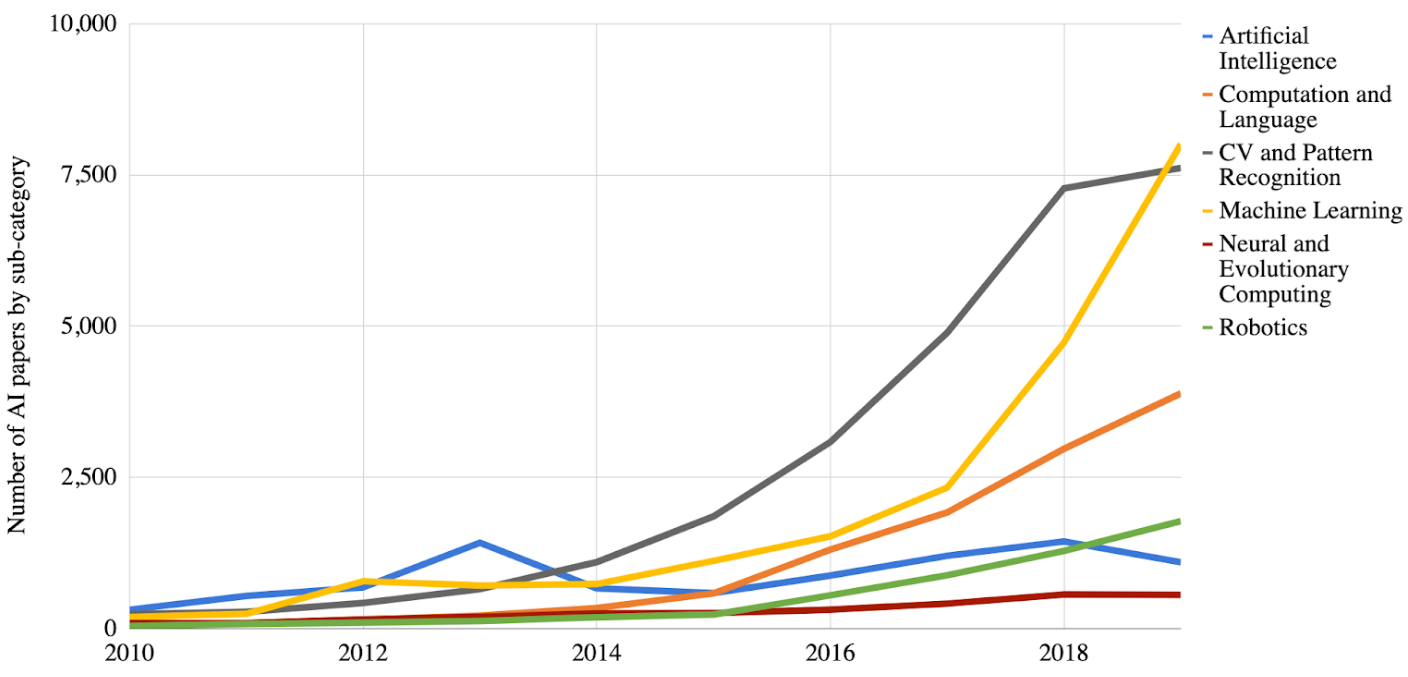
\includegraphics[width=0.7\textwidth]{diagrams/6-cvn/papers.png}
    \caption[papers short]
    {The number of artificial intelligence papers submitted to arXiv, broken down by sub-category.
        Note the particularly large increase in Computer Vision (CV) and pattern recognition
        papers. Figure taken from Ref.\cite{perrault2019}.}
    \label{fig:papers}
\end{figure}

In 2016 the NoVA experiment applied a CNN to the task of classifying the interaction type of
events within their sampling calorimeter detector~\cite{aurisano2016}. Two views of raw detector
events were used as input to train a network based on the popular GoogLeNet
architecture~\cite{szegedy2015}, discussed in section \ref{sec:cvn_theory_conv}. An improved
iteration has since been applied to both the classification of individual energy deposit
clusters~\cite{psihas2019} and $\nu_{e}$ and $e^{-}$ energy reconstruction~\cite{baldi2019}.

CNNs have also been applied to liquid argon time-projection chambers. The MicroBooNE experiment
has shown that in addition to classification tasks, the localisation of single particles within
events is possible~\cite{acciarri2017}. Furthermore, the DUNE collaboration has designed a network
to output both the interaction class and counts of different particle types in an
event~\cite{collaboration2020, abi2020}. This approach is called \emph{multi-task} learning and is
discussed in detail within Section.~\ref{sec:cvn_baseline_outputs}.

Applications to water Cherenkov detectors have also been made, by both the Daya Bay reactor
experiment~\cite{racah2016} and the KM3NeT/ORCA collaboration~\cite{aiello2020}. Additionally, a
type of network known as a \emph{variational autoencoder} has been shown to approximate the
distribution of simulated water Cherenkov data~\cite{abhishek2019}. If further studies prove
successful, this could allow for training on real data to reduce experimental uncertainties and
increase the speed of simulated data generation by many orders of magnitude.

\section{Standard event reconstruction and classification} %%%%%%%%%%%%%%%%%%%%%%%%%%%%%%%%%%%%%%%
\label{sec:cvn_old} %%%%%%%%%%%%%%%%%%%%%%%%%%%%%%%%%%%%%%%%%%%%%%%%%%%%%%%%%%%%%%%%%%%%%%%%%%%%%%

It is essential to outline the standard event reconstruction and classification methods that have
been used by the \chips project until now, for two main reasons. Firstly, to add context for
comparison with the new CNN approach, as is done in Section~\ref{sec:cvn_results_comparison}.
Secondly, to highlight the main weaknesses of these methods, motivating the new technique and
making its advantages clear.

A \emph{maximum likelihood} method based on that implemented by MiniBooNE~\cite{patterson2009} is
used for event reconstruction. Additionally, a simple neural network built using the TMVA
package~\cite{hocker2007} and using outputs from the reconstruction is used for event
classification. Both methods are very typical of the mainstream approach used by the majority of
water Cherenkov neutrino experiments. A prime example is the fiTQun algorithm developed for the
Super-Kamiokande detector, which is now used for both atmospheric~\cite{jiang2019} and
T2K~\cite{missert2017} analyses.

\subsection{Likelihood based reconstruction} %%%%%%%%%%%%%%%%%%%%%%%%%%%%%%%%%%%%%%%%%%%%%%%%%%%%%
\label{sec:cvn_old_reco} %%%%%%%%%%%%%%%%%%%%%%%%%%%%%%%%%%%%%%%%%%%%%%%%%%%%%%%%%%%%%%%%%%%%%%%%%

The event reconstruction methodology is simple in theory: for a given set of hypothesised tracks,
the number of photoelectrons and the time at which the first of these is recorded for each PMT in
the detector is predicted. By comparing this prediction with the measured hit charges and times
the likelihood that the given track hypothesis produced the measured signals can be calculated.
The parameters that describe the hypothesised tracks are then varied until the negative logarithm
of the likelihood is minimised. Identifying the best-fit parameters for the hypothesis. A brief
description of the procedure is given below, however, for a full description see
Ref.~\cite{blake2016} and in great detail Ref.~\cite{perch2017}.

\subsubsection*{Seeding} %%%%%%%%%%%%%%%%%%%%%%%%%%%%%%%%%%%%%%%%%%%%%%%%%%%%%%%%%%%%%%%%%%%%%%%%%

The first stage of event reconstruction is the effective \emph{seeding} of tracks that are then
used in the full likelihood fit. The seeding methods aim to provide a good starting point for the
minimisation, both to increase the efficiency of finding the optimal track parameters and also to
avoid a false local minimum from being returned.

Firstly, the PMT hits are sliced in both space and time. Gaps in the time ordering of hits are
used to separate the event into time slices. Each of these then undergoes basic filtering and
clustering to remove outlying hits and ensure only the dominant collections of hits are
considered. Each cleaned slice is then run through simple vertex finding algorithms to estimate
the interaction position and time, as well and the initial track direction.

A circular \emph{Hough transform} algorithm, traditionally used for water Cherenkov ring finding
is then applied. The voting-based transformation produces an output space within which rings of
PMT hits exist as single peaks. The track direction values are then further refined using this
space, and a search for smaller peaks is carried out to indicate if multiple particles are likely
to be involved. This process results in a list of seeds with a corresponding score related
directly to the height of the associated peak in Hough transform space.

\subsubsection*{Likelihood fit} %%%%%%%%%%%%%%%%%%%%%%%%%%%%%%%%%%%%%%%%%%%%%%%%%%%%%%%%%%%%%%%%%%%

Each track in a fit hypothesis is made up of a vector of parameters $\vec{x}$, containing the
following:
\begin{itemize}
    \item The track vertex position ($x_{0}$, $y_{0}$, $z_{0}$) and interaction time $t_{0}$.
    \item The initial track direction ($d_{\theta}$, $d_{\phi}$).
    \item The initial kinetic energy of the particle.
    \item The particle type (muon, electron or photon).
\end{itemize}
Additionally, for a photon hypothesis (identical to an electron hypothesis in reality) the
distance between the interaction vertex and the beginning of the electromagnetic shower is
included as a parameter.

The tracks in the hypothesis are then initialised using those found in the seeding procedure in
descending order of Hough peak height score. As the seeding algorithms do not estimate the
particle energy, a default value equal to the average particle energy observed in the Monte Carlo
simulation is assigned. Additionally, constraints can be placed on multi-track fits before the
minimisation process begins to reduce the number of free parameters.

For example, in the NC $\pi^{0}$ case, a multi-track two-photon hypothesis is used. Firstly, the
initial parameters for the two photons are assigned from the two highest-scoring seeds. Secondly,
the vertex position for both tracks is constrained to remain the same, and the directions and
energies are set to be constrained by the invariant mass of the $\pi^{0}$.

In it's simplest form the likelihood is a simple product of two terms:
\begin{equation} % LIKELIHOOD EQUATION %
    \mathcal{L}(\vec{x})=\mathcal{L}_{unhit}(\vec{x})\mathcal{L}_{hit}(\vec{x})=
    \prod_{unhit}P_{unhit}(\vec{x})\prod_{hit}P_{charge}(\vec{x})P_{time}(\vec{x}),
    \label{eq:likelihood}
\end{equation}
where the first ($unhit$) gives the likelihood that the hypothesis $\vec{x}$ will not predict a
hit on the PMTs that do not have a measured hit, and the second ($hit$) gives the likelihood that
$\vec{x}$ produces the observed photoelectrons and hit times on the hit PMTs. By considering the
negative logarithm of the likelihood instead, the computation can be simplified into a sum of
logarithms over the PMTs, such that
\begin{equation} % LIKELIHOOD SUM PMTS EQUATION %
    -\log\mathcal{L}(\vec{x})=
    -\sum_{unhit}\log(P_{unhit}(\vec{x}))
    -\sum_{hit}\log(P_{charge}(\vec{x}))
    -\sum_{hit}\log(P_{time}(\vec{x})).
    \label{eq:likelihood_sum}
\end{equation}
This also has the effect of separating the charge (number of photoelectrons) and time prediction
components which can then be dealt with separately computationally. In the actual likelihood
calculation the $P_{unhit}(\vec{x})$ and $P_{charge}(\vec{x})$ components are combined, where the
probability of an unhit PMT is treated as a PMT with observed charge equal to zero.

The Minuit2 algorithm contained within ROOT~\cite{brun1997} is used for the minimisation process.
At each iteration, the charge and hit time predictions are made, and the negative logarithm of the
likelihood is calculated. The track parameters are then varied to minimise the likelihood before
the next iteration. Through a series of stages, fixing and freeing specific parameters, the
minimisation process converges to the best-fit parameters for the given hypothesis. This process
typically takes two minutes on a standard batch farm computing node.

\subsubsection*{Downsides} %%%%%%%%%%%%%%%%%%%%%%%%%%%%%%%%%%%%%%%%%%%%%%%%%%%%%%%%%%%%%%%%%%%%%%%

The charge and hit time predictions and their associated likelihood contributions rely on many
low-level inputs to the reconstruction. These generally describe how Cherenkov light is emitted
from specific particles and then propagates through the detector to be detected by the PMTs.
Examples of these inputs include the following:
\begin{itemize}
    \item The number of Cherenkov photons emitted by a particle of specific type and energy.
    \item The fraction of Cherenkov light emitted at each step along a specific particles track
          length.
    \item The angular distribution of Cherenkov photon emission for each type of particle.
    \item The survival probability of photons within the detector medium as a function of
          distance.
    \item A detailed description of the PMT positions and directions within the detector.
    \item The angular efficiency of each PMT relative to the incident photon angle.
    \item The probability of a measured charge given the predicted number of photoelectrons
          (derived from a reversal of the simulation digitisation methodology).
\end{itemize}
The first three are combined into \emph{emission profiles} generated from large samples of the
Monte Carlo simulation, one representation of which is very similar to those shown in
Fig.~\ref{fig:emission_profile}. Additionally, the last listed input is comparable to that shown
in Fig.~\ref{fig:digitisation}.

The list above demonstrates a fundamental problem with the likelihood-based approach. It is
heavily reliant on the accuracy of low-level inputs and their associated use in human implemented
software. If a physical process is not dealt with appropriately or overlooked, then the prediction
accuracy of charges and hit times for the PMTs is affected, impacting the performance of finding
accurate best-fit parameters.

The other fundamental flaw of the likelihood-based approach is the requirement of a predefined
track hypothesis. Real events expected within \chips are rarely simple single particle or even
two-particle events. In reality, the majority of events contain multiple final state particles of
various types and in various topologies. The predefinition of a track hypothesis makes the
implementation of a generalised approach to event reconstruction where all possible event types
are considered impossible.

\subsection{Event classification}%%%%%%%%%%%%%%%%%%%%%%%%%%%%%%%%%%%%%%%%%%%%%%%%%%%%%%%%%%%%%%%%%
\label{sec:cvn_old_pid} %%%%%%%%%%%%%%%%%%%%%%%%%%%%%%%%%%%%%%%%%%%%%%%%%%%%%%%%%%%%%%%%%%%%%%%%%%

As the reconstruction is based on the calculation of a likelihood (analogous to a
\emph{goodness-of-fit}), the likelihood ratio between different hypotheses can be used for event
classification tasks. It is also found that additional hand-engineered features derived from the
reconstruction outputs have power in classifying the event type.

Two simple neural networks are used, the first for CC $\nu_{e}$ - CC $\nu_{\mu}$ separation and
the second for CC $\nu_{e}$ - NC separation. Both contain a single hidden layer, with the number
of nodes equal to the number of input parameters plus five. Variables from both a single $e$
track, and single $\mu$ track hypothesis fit to each event are used for both networks, with a full
list of inputs as follows:
\begin{itemize}
    \item The $\Delta\log\mathcal{L}$ between $e$ and $\mu$ hypothesis for both time and charge
          components.
    \item The total number of hit PMTs ($N_{hits}$) and total collected charge.
    \item $\frac{\Delta\log\mathcal{L}_{charge}}{N_{hits}}$.
    \item The fraction of hits inside, within, and outside the ring for both $e$ and $\mu$
          hypotheses.
    \item The fraction of predicted charge outside the ring for both $e$ and $\mu$ hypotheses.
    \item The ratio of the total predicted charged to the total measured charge for both $e$
          and $\mu$ hypothesis.
    \item The ratio of the reconstructed energy to the total measured charge.
    \item The reconstructed track direction under the $e$ hypothesis.
    \item The fraction of hits in the downstream half of the detector.
    \item The number of seeds generated by the Hough transform seeding algorithm.
    \item The peak height score of the first and last seeds found by the Hough transform seeding
          algorithm.
\end{itemize}

A sample of CC $\nu_{e}$ and CC $\nu_{\mu}$ beam events characteristic of those expected to be
seen by \chips is used to train the first classifier, and a corresponding sample of CC $\nu_{e}$
and NC events for the second. Both output values can then be used to classify events into separate
samples for further analysis.

The main limitation of this approach is that the input features are restricted to those that have
been imagined (requiring extensive domain knowledge) and then implemented in software. The current
list is undoubtedly non-exhaustive of all the possible variables and combinations of variables
that can, in theory, be used for discrimination between events. Additionally, any mistakes in the
likelihood-based reconstruction and, therefore, input variables to the neural networks, can lead
to incorrect categorisation of events.

\section{The theory of neural networks} %%%%%%%%%%%%%%%%%%%%%%%%%%%%%%%%%%%%%%%%%%%%%%%%%%%%%%%%%%
\label{sec:cvn_theory} %%%%%%%%%%%%%%%%%%%%%%%%%%%%%%%%%%%%%%%%%%%%%%%%%%%%%%%%%%%%%%%%%%%%%%%%%%%

There are many machine learning techniques: linear regression, logistic regression, k-nearest
neighbours, decision trees, random forests, support vector machines, all of which learn to make
predictions about data. However, none have been as successful, especially in recent years, as the
deep neural network. As both the size of datasets and the amount of available computational power
has increased, deep neural networks have proven the most powerful technique for many tasks as they
are well suited to this paradigm.

Here we discuss the application of neural networks for \emph{supervised learning}, one of two
broad machine learning categories that is concerned with using labelled example data to train
algorithms. The other category of \emph{unsupervised learning}, where the properties of the
dataset are inferred without example data is not discussed, however, will be used
Section.~\ref{sec:cvn_explain}.

\subsection{Neural network basics} %%%%%%%%%%%%%%%%%%%%%%%%%%%%%%%%%%%%%%%%%%%%%%%%%%%%%%%%%%%%%%%
\label{sec:cvn_theory_basics} %%%%%%%%%%%%%%%%%%%%%%%%%%%%%%%%%%%%%%%%%%%%%%%%%%%%%%%%%%%%%%%%%%%%

A neural network is a type of algorithm inspired by the repeating cell structure of neurons within
our brains. The basic building block of a neural network is a \emph{neuron} which takes a vector
of $k$ inputs $\vec{x} = (x_{1}, x_{2},\dots,x_{k})$ and outputs a scalar $a(\vec{x})$. The
neurons are arranged into layers, with the input of one layer being the output from the previous
layer. The first layer is commonly referred to as the \emph{input layer}, the middle layers as
\emph{hidden layers}, and the final layer as the \emph{output layer}, as illustrated in
Fig.~\ref{fig:network}. In general, this simple neural network structure is referred to as
\emph{fully-connected} as all the neurons in each layer have connections to all the neurons in the
previous and following layers.

\begin{figure} % BASIC NETWORK DIAGRAM %
    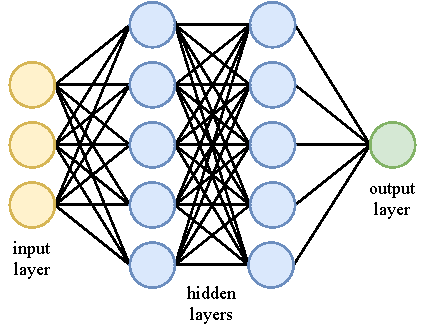
\includegraphics[width=0.7\textwidth]{diagrams/6-cvn/network.pdf}
    \caption[Illustration of a simple neural network]
    {Illustration of a simple neural network. There is a single input layer (yellow), two hidden
        layers (blue), and an output layer (green). Each node corresponds to a \emph{neuron}
        except for the input layer.}
    \label{fig:network}
\end{figure}

Input variables (traditionally hand-engineered features extracted from the raw data) are passed
into the network via the input layer. Any number of hidden layers containing any number of neurons
can then follow. The neurons contained within these layers are trained so that collectively their
$a(\vec{x})$ functions solve the task at hand. For a \emph{regression} task, the output layer
outputs a continuous decimal value. Otherwise, for a \emph{classification} task, a probability
value between zero and one is output for each class. The forward passing of information from one
layer to the next is why neural networks can also be referred to as \emph{feed-forward graphs}.

For a neuron $i$, $a_{i}(\vec{x})$ can be decomposed into a linear operation, specific to the
neuron, followed by a non-linear operation, which is the same across all neurons. The linear
operation consists of the dot product of the input vector $\vec{x}$ with a vector of weights
$\vec{w}^{(i)} = (w_{1}^{(i)}, w_{2}^{(i)},\dots,w_{k}^{(i)})$, plus a bias term $b^{(i)}$:
\begin{equation} % NETWORK BASIC EQUATION %
    z^{(i)}=\vec{w}^{(i)}\cdot\vec{x}+b^{(i)}.
    \label{eq:network}
\end{equation}
After applying the non-linear operation $\sigma_{i}$, commonly referred to as the \emph{activation
    function} the final output from the neuron can be written as
\begin{equation} % NETWORK ACTIVATION EQUATION %
    a_{i}(\vec{x})=\sigma_{i}(z^{(i)}).
    \label{eq:activation}
\end{equation}

Traditionally, a step-function (for networks called \emph{perceptrons}) was used for the
activation function. However, as is shown in Section.~\ref{sec:cvn_theory_training}, a non-zero
gradient (only valid at $x=0$ for a step-function) is required for the practical training of
neural networks. In fact, the choice of activation function can greatly affect how the network
trains and performs.

Therefore, common choices have been the \emph{hyperbolic tangent} and the \emph{sigmoid} function,
primarily because they are bounded and differentiable at all points. Recently, the \emph{ReLU} and
other similar functions have become popular, especially for CNNs. This is mainly due to them
avoiding the problem of \emph{vanishing} gradients caused by the saturation of the tanh and
sigmoid functions at large values of $x$. All of these functions are shown in
Fig.~\ref{fig:activations}.

\begin{figure} % ACTIVATIONS DIAGRAM %
    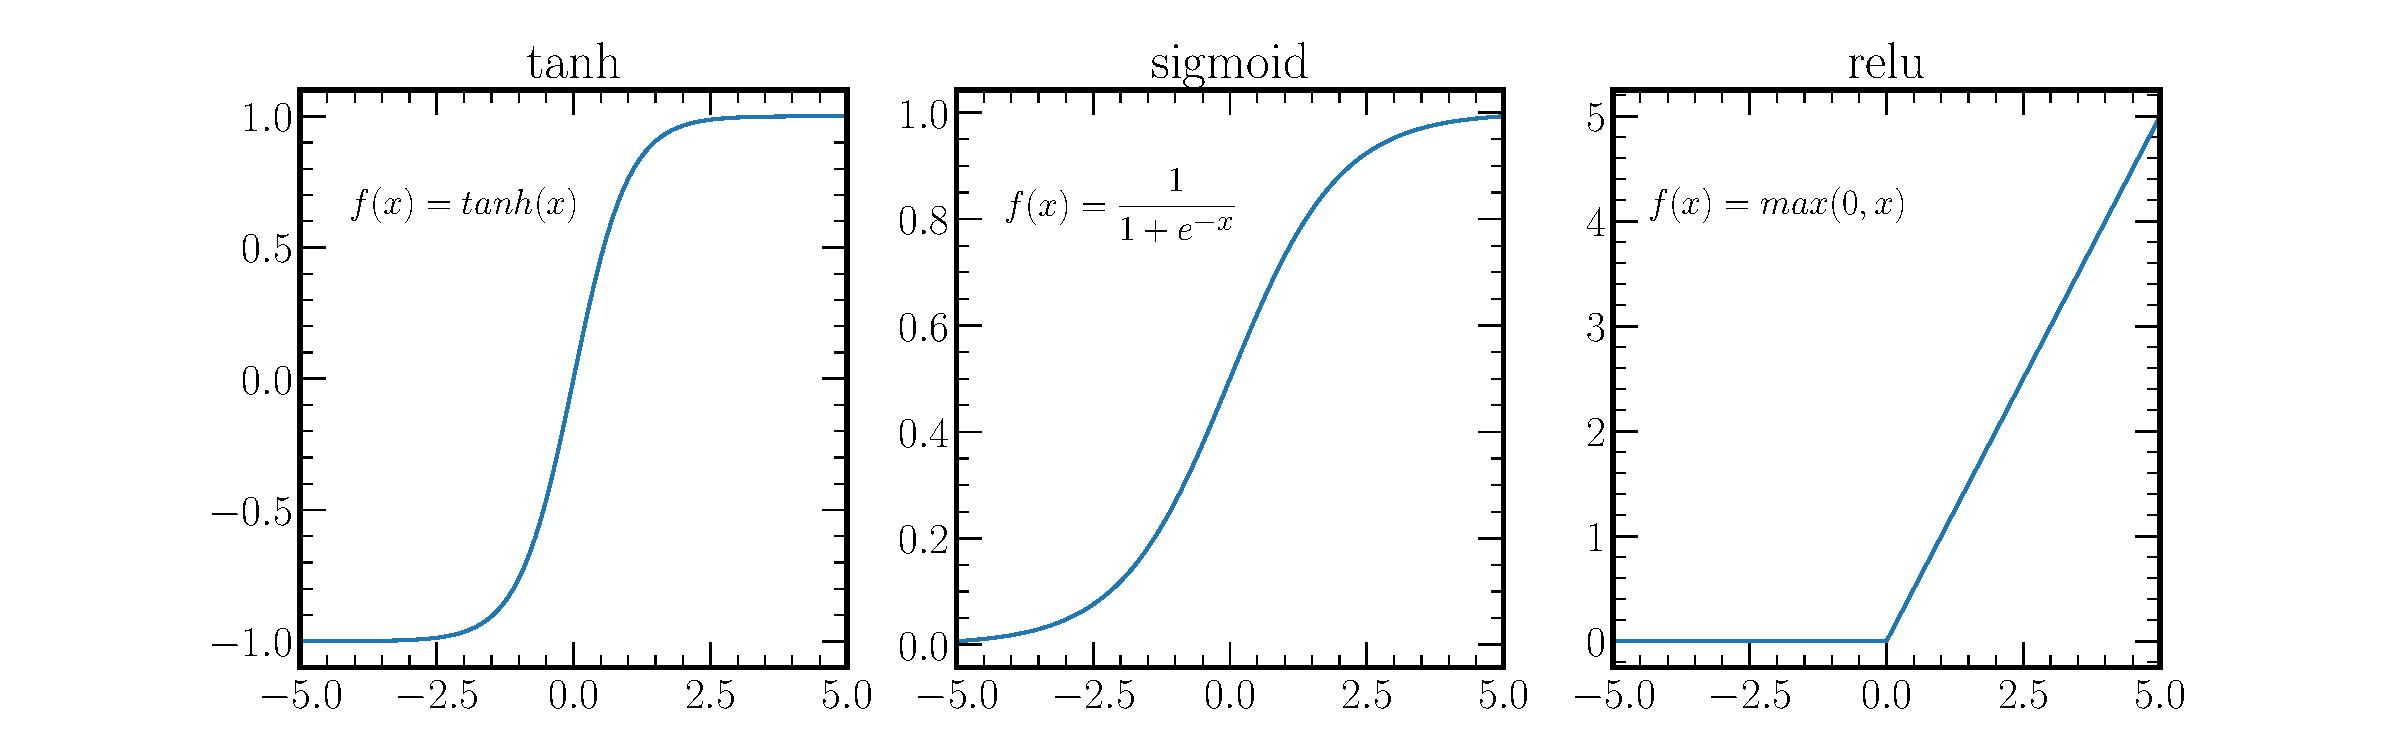
\includegraphics[width=\textwidth]{diagrams/6-cvn/activations.pdf}
    \caption[Common non-linear activation functions.]
    {Common non-linear activation functions used for the neurons within neural networks.}
    \label{fig:activations}
\end{figure}

\subsection{Training neural networks} %%%%%%%%%%%%%%%%%%%%%%%%%%%%%%%%%%%%%%%%%%%%%%%%%%%%%%%%%%%%
\label{sec:cvn_theory_training} %%%%%%%%%%%%%%%%%%%%%%%%%%%%%%%%%%%%%%%%%%%%%%%%%%%%%%%%%%%%%%%%%%

The process of supervised training of a neural network uses labelled data to iteratively find the
optimal weights and biases (network parameters) that maximise the network performance. In order to
quantify the performance, we must define a \emph{loss function} $E(\vec{w})$, where $\vec{w}$ is
the vector of network parameters, describing the difference between the network output and the
true label. For a given input data point $(\vec{x}_{i}, y_{i})$, where $\vec{x}_{i}$ are the input
parameters and $y_{i}$ is the known truth label, the network generates an output
$\hat{y}_{i}(\vec{w})$. Using this notation, we can then construct loss functions suitable for
different tasks.

In the case of a simple binary classification task, the most commonly used function is the
\emph{binary cross-entropy}:
\begin{equation} % BINARY CROSS-ENTROPY EQUATION %
    E(\vec{w})=
    -\displaystyle\sum_{i=1}^{n}y_{i}\log\hat{y}_{i}(\vec{w})+
    (1-y_{i})\log[1-\hat{y}_{i}(\vec{w})],
    \label{eq:binary_cross_entropy}
\end{equation}
where the number of data points is given by $n$. For a classification task where the number of
classes is greater than two $y$ can take on $M$ values. In this case we redefine each data point
so that $y$ is instead a vector $y_{im}$ such that
\begin{equation} % ONE-HOT EQUATION %
    y_{im}=
    \begin{cases}
        1 & \text{if $y_{i}=m$} \\
        0 & \text{otherwise.}   \\
    \end{cases}
\end{equation}
This is commonly named a \emph{one-hot} vector. The cross-entropy then becomes the
\emph{categorical cross-entropy}:
\begin{equation} % CATEGORICAL CROSS-ENTROPY EQUATION %
    E(\vec{w})=
    -\displaystyle\sum_{i=1}^{n}\displaystyle\sum_{m=0}^{M-1}y_{im}\log\hat{y}_{im}
    (\vec{w})+(1-y_{im})\log[1-\hat{y}_{im}(\vec{w})].
    \label{eq:categorical_cross_entropy}
\end{equation}
For a regression task predicting a continuous output variable, the \emph{mean-squared error} is
most often used as the loss function:
\begin{equation} % MEAN-SQUARED ERROR LOSS EQUATION %
    E(\vec{w})=
    \frac{1}{n}\displaystyle\sum_{i=1}^{n}(y_{i}-
    \hat{y}_{i}(\vec{w}))^{2}.
    \label{eq:mse}
\end{equation}

To find the optimal network parameters for the given task we can iteratively minimise the loss
function until it converges to its minimum (or in reality a local minimum that performs well).
This is done by updating the network parameters at each iteration $t$ to move in the direction of
the gradient of the loss function using an update rule:
\begin{equation} % UPDATE EQUATION %
    \vec{w}_{t+1}=\vec{w}_{t}-\eta_{t}\nabla_{\vec{w}}E(\vec{w}),
    \label{eq:update_rule}
\end{equation}
where $\eta_{t}$ is the \emph{learning rate}, determining the size of the step taken at each
iteration. This methodology is known as \emph{gradient descent} and is illustrated in
Fig.~\ref{fig:gradient_descent}.

\begin{figure} % GRADIENT DESCENT DIAGRAM %
    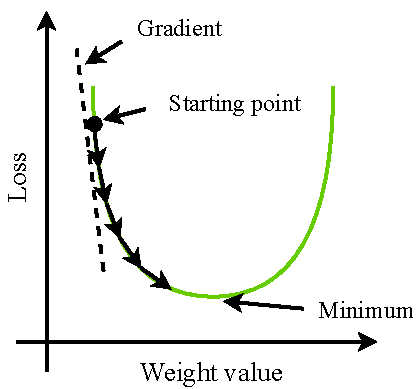
\includegraphics[width=0.5\textwidth]{diagrams/6-cvn/gradient_descent.pdf}
    \caption[Illustration of the gradient descent process.]
    {Simplified illustration of the gradient descent procedure. Shown is the case for a loss
        function dependent on a single weight.}
    \label{fig:gradient_descent}
\end{figure}

Therefore, in order to use gradient descent, we require that the gradient of the loss function
with respect to the parameters of the network can be calculated. Doing this for each parameter at
every iteration would render neural networks impossible to train due to the vast computational
requirements. Instead, an innovative application of the chain rule in an algorithm called
\emph{backpropagation} is used~\cite{werbos1974}. Here we follow the derivation of the four main
equations of backpropagation from Ref.~\cite{mehta2019}.

For a network containing $L$ layers, we can index the individual layers using $l=1,\dots,L$. The
weight associated with the connection between the $k$-th neuron in layer $l-1$ and the $j$-th
neuron in layer $l$ can be denoted as $w^{l}_{jk}$. The bias of the layer $l$ neuron is written as
$b^{l}_{j}$. The activation of the $j$-th neuron in layer $l$ is then related to the outputs from
the previous layer by
\begin{equation} % PREVIOUS LAYER EQUATION %
    a^{l}_{j}=\sigma(z^{l}_{j})=\sigma\left(\sum_{k}w^{l}_{jk}a^{l-1}_{k}+b^{l}_{j}\right).
    \label{eq:feedforward}
\end{equation}

The change in the loss function with respect to the linear weighted sum $z^{l}_{j}$ of the $j$-th
neuron in the last layer $L$ can be used to define the error:
\begin{equation} % PREVIOUS LAYER EQUATION %
    \Delta^{L}_{j}=\frac{\partial E}{\partial z^{L}_{j}}.
\end{equation}
Similarly the error on any neuron $j$ in any layer $l$ is given by
\begin{equation} % BACKPROP EQUATION 1 %
    \Delta^{l}_{j}=\frac{\partial E}{\partial z^{l}_{j}}=\frac{\partial E}{\partial a^{l}_{j}}
    \sigma '(z^{l}_{j}),
    \label{eq:backprop_1}
\end{equation}
with $\sigma '$ denoting the derivative of the non-linear activation function. As $\partial
    b^{l}_{j}/\partial z^{l}_{j}=1$, the error can also be viewed as the partial derivative of the
loss function with respect to the bias:
\begin{equation} % BACKPROP EQUATION 2 %
    \Delta^{l}_{j}=\frac{\partial E}{\partial z^{l}_{j}}
    =\frac{\partial E}{\partial b^{l}_{j}}\frac{\partial b^{l}_{j}}{\partial z^{l}_{j}}
    =\frac{\partial E}{\partial b^{l}_{j}}.
    \label{eq:backprop_2}
\end{equation}

Using the chain rule and the fact that the error on neurons in layer $l$ only depends on the
activation of neurons in the following layer $l+1$, we can write
\begin{align} % BACKPROP EQUATION 3 %
    \begin{split}
        \Delta^{l}_{j} &=\frac{\partial E}{\partial z^{l}_{j}}
        =\sum_{k}\frac{\partial E}{\partial z^{l+1}_{k}}
        \frac{\partial z^{l+1}_{k}}{\partial z^{l}_{j}} \\
        &=\sum_{k}\Delta^{l+1}_{k}\frac{\partial z^{l+1}_{k}}{\partial z^{l}_{j}} \\
        &=\left(\sum_{k}\Delta^{l+1}_{k}w^{l+1}_{kj}\right)\sigma '(z^{l}_{j}).
    \end{split}
    \label{eq:backprop_3}
\end{align}
Additionally, the differential of the cost function with respect to the weight $w^{l}_{jk}$ can be
written as
\begin{equation} % BACKPROP EQUATION 4 %
    \frac{\partial E}{\partial w^{l}_{jk}}
    =\frac{\partial E}{\partial z^{l}_{j}}\frac{\partial z^{l}_{j}}{\partial w^{l}_{jk}}
    =\Delta^{l}_{j}a^{l-1}_{k}.
    \label{eq:backprop_4}
\end{equation}

The full backpropagation algorithm then proceeds as follows:
\begin{enumerate}
    \item After calculating the activations $a^{1}_{j}$ for all neurons in the input layer, use
          the feed-forward architecture of the network to calculate all activations at every layer
          using Eq.~\ref{eq:feedforward}.
    \item Use Eq.~\ref{eq:backprop_1} to calculate the error of the top layer neurons. Both the
          derivative of the loss function and the activation function is required for this step.
    \item Use Eq.~\ref{eq:backprop_2} to `backpropagate' the error through the network from the
          top layer to the input layer to find all $\Delta^{l}_{j}$ values.
    \item Calculate the gradients for all the weights and biases using Eq.~\ref{eq:backprop_3} and
          Eq.~\ref{eq:backprop_4}.
\end{enumerate}
As can be seen, a single activation finding \emph{forward pass} followed by a single error
propagating \emph{backward pass}  is all that's required to calculate the gradients for all
weights and biases within the network. This incredibly efficient procedure allows for the use of
gradient descent to train neural networks.

\subsection{Convolutional neural networks} %%%%%%%%%%%%%%%%%%%%%%%%%%%%%%%%%%%%%%%%%%%%%%%%%%%%%%%
\label{sec:cvn_theory_conv} %%%%%%%%%%%%%%%%%%%%%%%%%%%%%%%%%%%%%%%%%%%%%%%%%%%%%%%%%%%%%%%%%%%%%%

The broad category of deep learning covers multiple neural network techniques spanning a range of
application fields such as computer vision, speech recognition and natural language processing. By
stacking many layers on top of each other into a `deep' network, these methods offer increased
problem-solving capacity by allowing higher-order non-linear functions to form. As a direct
consequence, instead of requiring hand-engineered features as input, deep networks can learn to
extract the most powerful features from raw data. Here we outline just the technique used in this
work; the convolutional neural network (CNN).

At their core, a CNN makes use of a mathematical operation called \emph{convolution}, which either
entirely or in part replaces the simple vector multiplication seen in fully-connected networks as
introduced in Section~\ref{sec:cvn_theory_basics}. This difference makes CNNs incredibly powerful
for applications using grid-like input data such as computer vision tasks.

Using standard CNN terminology, the discrete convolution between the \emph{input}, $x$ and the
\emph{kernel}, $w$ is given by
\begin{equation}
    f_{i}=(x*w)_{i}=\sum^{\infty}_{j=-\infty}x_{j}w_{i-j},
    \label{eq:convolution}
\end{equation}
where $f$ is commonly referred to as the \emph{feature map}. In typical applications, the input is
a two-dimensional array $X$. Therefore, both the kernel, $W$ and the resulting feature map, $F$
also become two-dimensional. In this case the convolution operation becomes
\begin{equation}
    F_{i}=(X*W)_{i,j}=\sum_{m}\sum_{n}X_{i+m,j+n}W_{m,n},
    \label{eq:conv}
\end{equation}
where the infinite sum in Eq.~\ref{eq:convolution} has been replaced with a discrete sum over
two-dimensional elements. Normally, the output feature map is then passed through a non-linear
activation function. Analogous to the simple neural network weights $\vec{w}$ first described in
Eq.~\ref{eq:network}, the elements of $W_{m,n}$ can be trained to maximise the network performance
(minimise the loss).

To illustrate this operation Fig.~\ref{fig:conv_input} gives examples of a $4 \times 4$ input grid
and a $3 \times 3$ kernel. The output feature map is generated by sliding the kernel across both
dimensions of the input grid, summing the products of all associated elements at each step
according to Eq.~\ref{eq:conv}, as shown in Fig.~\ref{fig:conv_operation}.

\begin{figure} % CONV INPUTS DIAGRAM %
    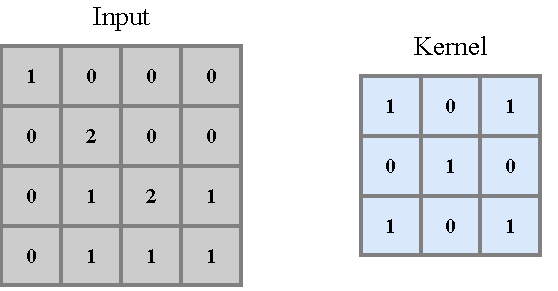
\includegraphics[width=0.7\textwidth]{diagrams/6-cvn/conv_input.pdf}
    \caption[Example of an input grid and kernel.]
    {Example of an input grid (left) and kernel (right). The specific kernel shown is sensitive to
        x-shaped features}
    \label{fig:conv_input}
\end{figure}

\begin{figure} % CONV OPERATION DIAGRAM %
    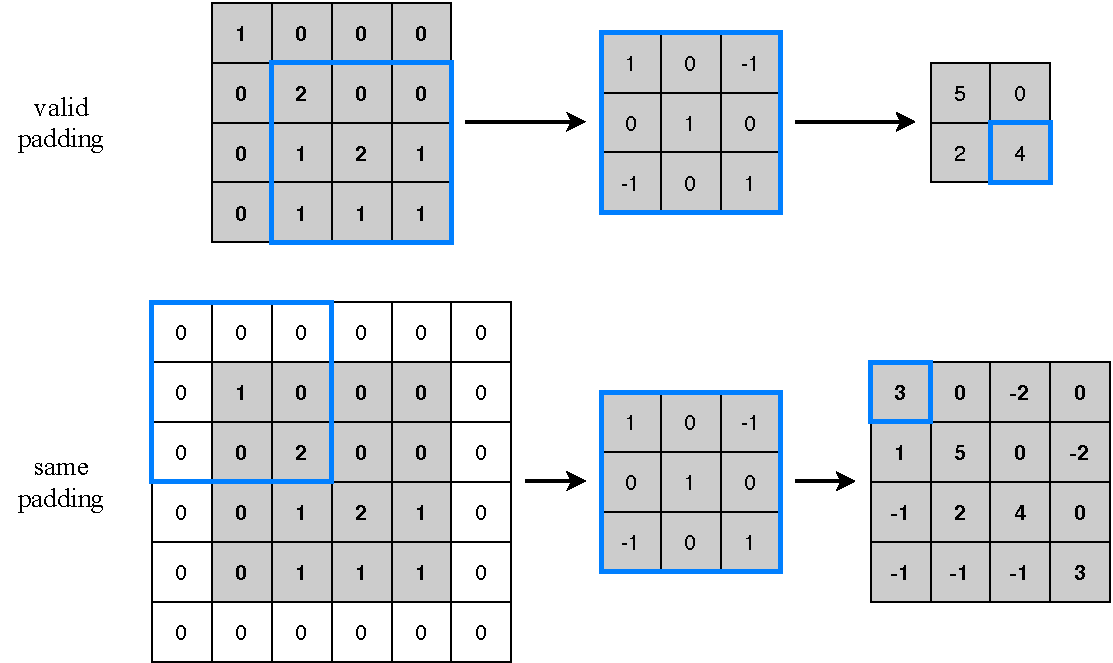
\includegraphics[width=0.7\textwidth]{diagrams/6-cvn/conv_operation.pdf}
    \caption[Example of convolutional operation.]
    {Example of a $\mathrm{stride}=1$ convolution operation involving the input grid and kernel
        from Fig.~\ref{fig:conv_input}. Both the operation for the case of \emph{valid} (top) and
        \emph{same} (bottom) padding is shown. The blue square in the top-left of the output
        feature maps indicates the output generated from the specific operation shown on the left
        also in blue.}
    \label{fig:conv_operation}
\end{figure}

Two additional parameters that impact the output size of the feature map are also introduced in
Fig.~\ref{fig:conv_operation}. The \emph{stride} and the \emph{padding}. The stride governs how
far the kernel moves at each step while the padding decides how the input grid is padded with
zeros around its border. If $L$ is the size of the input (both height and width) and $K$ is the
kernel size, the output feature map size $O$ is given by
\begin{equation}
    O=\frac{(L-K+2P)}{S}+1,
    \label{eq:conv_size}
\end{equation}
where $S$ is the stride, and $P$ is the amount of zero padding.

The other key operation used in CNNs is pooling. Pooling layers coarse-grain the spatial
information of the input via down-sampling to reduce the number of network parameters. \emph{Max
    pooling} or \emph{average pooling} are the two common ways this is achieved. In both cases, the
input is first divided into rectangular regions, and then either the maximum or average value of
the region is used as output, for max and average pooling respectively. As illustrated in
Fig.\ref{fig:pooling}.

\begin{figure} % POOLING DIAGRAM %
    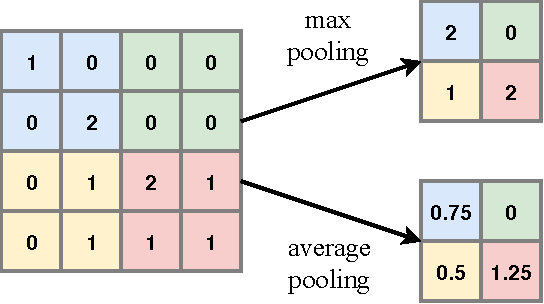
\includegraphics[width=0.7\textwidth]{diagrams/6-cvn/pooling.pdf}
    \caption[Example of pooling operation.]
    {Example of both a max and average $2 \times 2$ pooling operation with $\mathrm{stride}=2$.}
    \label{fig:pooling}
\end{figure}

Taking inspiration from how neurons behave in the visual cortex of animals~\cite{lecun2015}, small
kernels are generally used that only scan over a small spatial patch of the input at any one time.
When combined with the loss of absolute position information from pooling, a key feature of CNNs
is highlighted. They exhibit translational invariance and respect the local structure contained
within the input. In simpler terms, they do not care wherein the input image a particular feature
exists, just that it exists.

\subsubsection*{CNN architectures}

In 2012 the AlexNet CNN lowered the error rate of the ubiquitous ImageNet classification
task~\cite{deng2009} from 28\% to 16\%~\cite{krizhevsky2012}. Since this breakthrough, the
standard CNN has adopted a similar architecture. Multiple convolutional layers are stacked on top
of each other, periodically interspersed with pooling layers. Once the output feature map size no
longer allows for additional pooling, one or more fully-connected layers are added before the
final output layer, as shown in Fig.~\ref{fig:conv_diagram}.

\begin{figure} % CONV DIAGRAM %
    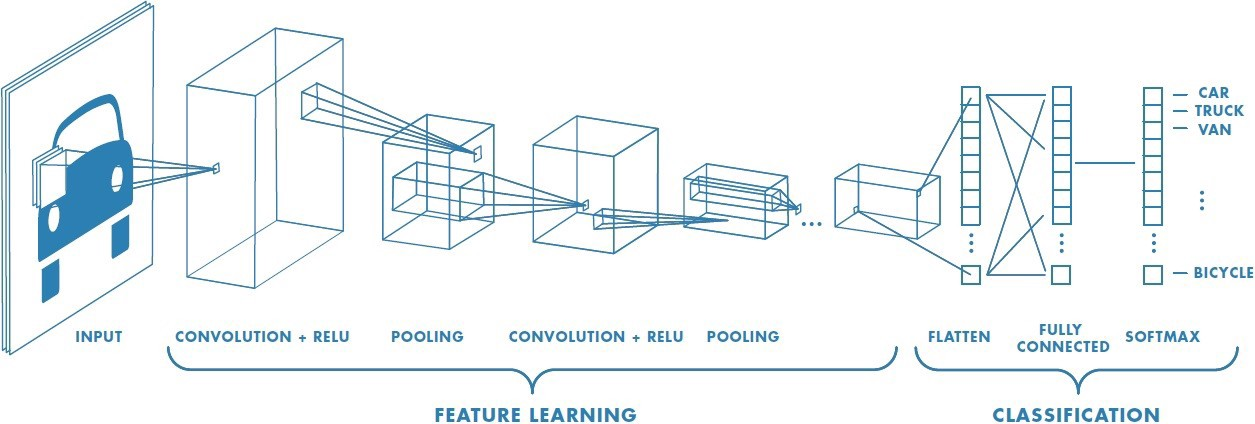
\includegraphics[width=\textwidth]{diagrams/6-cvn/conv_diagram.jpeg}
    \caption[Typical CNN architecture]
    {Illustration of a typical CNN architecture, containing convolutional, pooling and
        fully-connected layers before the final output layer.}
    \label{fig:conv_diagram}
\end{figure}

Led by research teams at the technology giants, improvements upon this standard architecture have
been made. Initially, this involved the addition of extra convolutional layers to form a deeper
network as VGG did in 2014~\cite{simonyan2014}. Separately, the \emph{inception module} introduced
by GoogLeNet~\cite{szegedy2015} the same year allowed for different scales of features to be
explored using the concept of a \emph{network-within-a-network}.

As the size of CNNs increased, it was found that the gradients on the lower layers of the network
were found to decrease. This sometimes had the effect of the gradient \emph{vanishing} from these
layers preventing learning. To counter this problem ResNet~\cite{he2016_original, he2016_improved}
introduced residual connections, skipping specific layers and allowing for a larger gradient to
reach the affected lower layers during backpropagation. Recently the inception module and ResNet
ideas have been combined~\cite{szegedy2016}, and there has been a significant push for efficient
rather than just deeper networks~\cite{sandler2018,tan2019}. The repeating layout of layers that
form the above networks, often referred to as \emph{blocks}, are shown in Fig.~\ref{fig:blocks}.

\begin{figure} % BLOCKS DIAGRAM %
    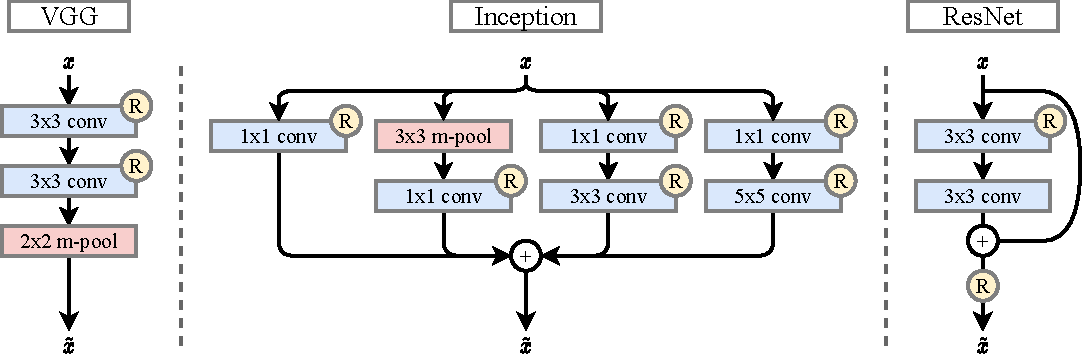
\includegraphics[width=\textwidth]{diagrams/6-cvn/blocks.pdf}
    \caption[Common CNN architecture blocks]
    {Common blocks used within CNN architectures, taking $x$ as input and producing $\tilde{x}$ as
        output through operations whose flow is described with the arrows. The blue and red boxes
        represent convolutional (conv) and max pooling (m-pool) layers respectively, with the size
        of the operation shown. The circular yellow $R$ indicates the use of the ReLU activation
        function.}
    \label{fig:blocks}
\end{figure}

\subsection{Regularisation} %%%%%%%%%%%%%%%%%%%%%%%%%%%%%%%%%%%%%%%%%%%%%%%%%%%%%%%%%%%%%%%%%%%%%%
\label{sec:cvn_theory_reg} %%%%%%%%%%%%%%%%%%%%%%%%%%%%%%%%%%%%%%%%%%%%%%%%%%%%%%%%%%%%%%%%%%%%%%%

A key challenge for supervised machine learning techniques is ensuring the algorithm can
generalise to new, previously unseen datasets. This can be difficult when for a deep neural
network containing millions of trainable parameters, it can become easy for the network to learn
the specific features and noise of the training dataset. This process is called \emph{overfitting}
and is very common when training CNNs. Methods used within this work to prevent this from
happening are outlined below, all of which are commonly referred to as \emph{regularisation}
techniques.

\subsubsection*{Stochastic Gradient Descent} %%%%%%%%%%%%%%%%%%%%%%%%%%%%%%%%%%%%%%%%%%%%%%%%%%%%%

The procedure outlined so far of updating the network weights at each training iteration using the
gradient calculated over the full dataset is called \emph{batch training}. It is instead much more
common to calculate an approximation to the gradient at each iteration using a \emph{minibatch} of
the full dataset. This is done by considering just a subset of the training data with a size
commonly referred to as the \emph{batch size} and typically equal to a power of two for
computational reasons.

This modification to standard gradient descent is called \emph{stochastic gradient descent} as it
introduces stochasticity to the training process, and provides two main advantages. Firstly the
computational speed of each iteration is significantly reduced, and crucially the memory
requirements lowered. Secondly, the addition of noise decreases the chance that the minimisation
will get stuck in a local minimum suited to overfitting the training dataset.

\subsubsection*{Early stopping} %%%%%%%%%%%%%%%%%%%%%%%%%%%%%%%%%%%%%%%%%%%%%%%%%%%%%%%%%%%%%%%%%%

\emph{Early stopping} is a simple procedure preventing overfitting from affecting the final
generalised performance of the network. During training, the training dataset is commonly iterated
over multiple times, with each iteration called an \emph{epoch}. By evaluating the error on an
independent \emph{validation} dataset at the end of each epoch, the point at which overfitting
begins can be determined, as shown in Fig.~\ref{fig:early_stopping}. At this point, the training
is stopped to return the best possible generalised model. In practice, it is common only to stop
training after $n$ number of epochs have passed with no validation error improvement.

\begin{figure} % EARLY STOPPING DIAGRAM %
    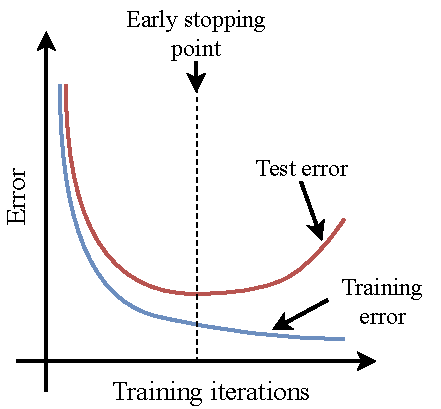
\includegraphics[width=0.5\textwidth]{diagrams/6-cvn/early_stopping.pdf}
    \caption[Illustration of the early stopping procedure.]
    {Illustration of the early stopping procedure. Initially both the training and test error
        decreases, but, at some point the test error will start to increase due to overfitting, at
        this point the training is stopped.}
    \label{fig:early_stopping}
\end{figure}

\subsubsection*{Batch normalisation} %%%%%%%%%%%%%%%%%%%%%%%%%%%%%%%%%%%%%%%%%%%%%%%%%%%%%%%%%%%%%

The training of a neural network is found to work best when the inputs of each neuron are centred
on zero with respect to the bias of the neuron. This is because large input values can cause
saturation of the activation function and subsequent \emph{vanishing} of the associated gradient,
reducing the ability of the network to learn. To counter this, \emph{batch normalisation}
introduces layers that standardise the inputs using the mean and variance calculated over each
minibatch~\cite{ioffe2015}. This not only speeds up training by preventing the \emph{vanishing} of
gradients but also reduces overfitting by using the stochasticity of the minibatch.

\subsubsection*{Dropout} %%%%%%%%%%%%%%%%%%%%%%%%%%%%%%%%%%%%%%%%%%%%%%%%%%%%%%%%%%%%%%%%%%%%%%%%%

\emph{Dropout} is another simple technique to reduce overfitting~\cite{hinton2012}. At each
training iteration, each neuron has a probability $p_{d}$ to be \emph{dropped out} and ignored for
that iterations calculation. This is illustrated in \ref{fig:dropout}. By ignoring a subset of the
neurons at each iteration it is difficult for the network to form the particularly strong
connections between neurons that are responsible for overfitting, leading to greater
generalisation.

\begin{figure} % DROPOUT DIAGRAM %
    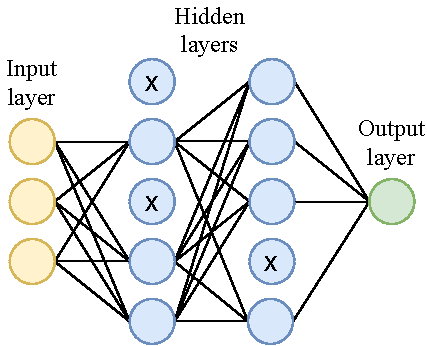
\includegraphics[width=0.7\textwidth]{diagrams/6-cvn/dropout.pdf}
    \caption[Illustration of dropout.]
    {Example of dropout applied to the network shown in Fig.~\ref{fig:network}. Neurons are
        randomly \emph{dropped out} and not considered at each training step. This reduces the
        strong correlations between neurons that can lead to overfitting.}
    \label{fig:dropout}
\end{figure}

\section{A baseline implementation for CHIPS} %%%%%%%%%%%%%%%%%%%%%%%%%%%%%%%%%%%%%%%%%%%%%%%%%%%%
\label{sec:cvn_baseline} %%%%%%%%%%%%%%%%%%%%%%%%%%%%%%%%%%%%%%%%%%%%%%%%%%%%%%%%%%%%%%%%%%%%%%%%%

The output from a water Cherenkov detector such as \chips is a simple image of each event where
two channels of information are known for each PMT: the number of collected photoelectrons, and
the associated hit times. Therefore, it is a natural fit to use CNNs primarily developed for
image-based computer vision tasks for \chips event analysis.

For this purpose, a Python-based software package named \emph{chipsnet}~\cite{chipsnet2020} has
been built. By using the high-level \emph{Application Programming Interfaces}, (APIs) provided by
the Tensorflow framework (initially developed by Google)~\cite{tf2015}, a full pipeline including
data preparation, network training, and performance evaluation is implemented. In this section,
the baseline CNN implementation built into chipsnet is outlined. The specific network
implementations described afterwards in Section.~\ref{sec:cvn_specific} for cosmic rejection, beam
classification, and energy estimation share this common baseline with a few specific differences.

\subsection{Baseline inputs} %%%%%%%%%%%%%%%%%%%%%%%%%%%%%%%%%%%%%%%%%%%%%%%%%%%%%%%%%%%%%%%%%%%%%
\label{sec:cvn_baseline_inputs} %%%%%%%%%%%%%%%%%%%%%%%%%%%%%%%%%%%%%%%%%%%%%%%%%%%%%%%%%%%%%%%%%%

The primary difficulty in the application of CNNs to \chips is determining how to map an event
captured on a cylindrical surface to a rectangular grid. Furthermore, this must be done in such a
way as not to distort the underlying event topology which could inhibit network learning. As a
solution, this work takes inspiration and then builds upon the ideas outlined in
Ref.~\cite{theodore2016}. Simply put, an event is mapped onto a two-dimensional grid as though it
is viewed from its estimated interaction vertex position. The primary motivation behind this is to
remove any detector shape effects and to focus on the underlying event topology and Cherenkov
emission profiles.

To estimate the interaction vertex position for each event, the top-scoring seed from the seeding
process introduced in Section~\ref{sec:cvn_old_reco} is used. This procedure, unlike the full
likelihood fit, requires no track hypothesis and typically takes under
\unit{0.5}{\mathrm{seconds}} per event on a standard batch farm computing node. The seed estimated
vertex position resolutions for a sample of expected beam events are shown in
Fig.~\ref{fig:explore_true_reco_vtx}. The $x$ component is commonly estimated closer to the
downstream wall of the detector than reality, however, as the $y$ and $z$ components perpendicular
to the beam primarily drive event distortions, the impact on event topology is small.

\begin{figure} % HOUGH VTX RES DIAGRAM %
    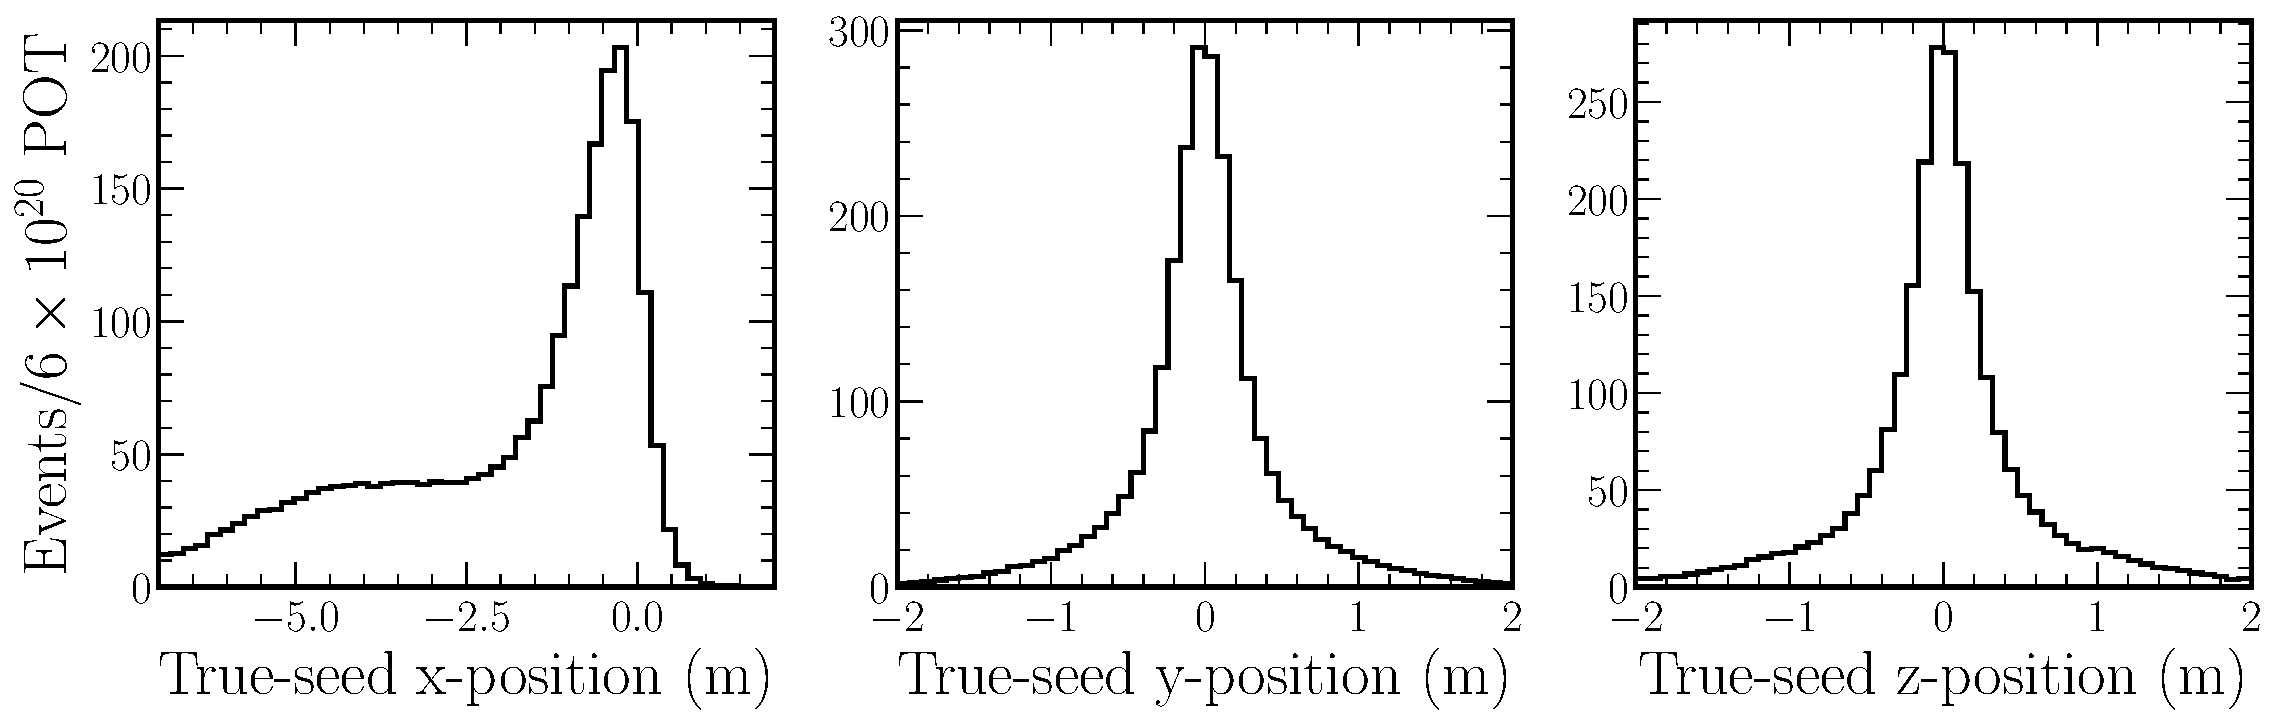
\includegraphics[width=\textwidth]{diagrams/6-cvn/chipsnet/explore_true_reco_vtx.pdf}
    \caption[Seed interaction vertex resolutions.]
    {$Truth - seed$ interaction vertex position resolution, split by component. The large negative
        tail for the $x$ component shows the tendency of the seeding procedure to estimate the $x$
        component closer to the downstream detector wall than reality.}
    \label{fig:explore_true_reco_vtx}
\end{figure}

Using $\theta$ and $\phi$ components calculated from the estimated interaction vertex position
facing along the x-axis (downstream), hit PMTs are mapped onto a $64 \times 64$ grid. This
procedure is used to generate two event \emph{maps}. Firstly, a \emph{hit-charge} map where each
grid bin is given by the total collected photoelectrons from all PMTs mapped to that bin.
Secondly, a \emph{hit-time} map where each grid bin is given by the first hit time (in ns) across
all PMTs mapped to that bin. Each hit-time map bin is additionally corrected so that the first hit
time in the event is at zero.

By design, the Hough transform within the seeding procedure uses the estimated interaction vertex
position to generate the transform space. Therefore, by re-binning the transform space to a $64
    \times 64$ grid a third \emph{hough-height} map is generated for each event. This event map aims
to provide a complementary but different representation of the event where Cherenkov rings are
instead represented as peaks, allowing for additional discriminating features to be learnt.

All three event maps: hit-charge, hit-time and hough-height, are down-sampled (from 32-bit floats)
using 8-bit encoding. This not only significantly reduces storage requirements but also
dramatically increases the speed with which data can be loaded during training (which turns out to
be the primary bottleneck). For each map type, a range over which to encode from zero up to a
\emph{cap-point} is chosen. This is selected to minimise the number of bin values that are capped
at the maximum encoded value of 255. Table.~\ref{tab:encoding} shows the cap-points, and
associated percentage of bin values capped for each map type, while
Fig.~\ref{fig:explore_8_bit_range} shows the distribution of bin values for each map across the
encoded range.

\begin{table}
    \begin{tabular}{lcc}
        Event map    & Cap-point & Capped percentage \\
        \midrule
        hit-charge   & 25 p.e    & 0.10\%            \\
        hit-time     & 120 ns    & 0.15\%            \\
        hough-height & 3500 p.e  & 0.23\%            \\
    \end{tabular}
    \caption[Table of input event map 8-bit cap-points]
    {Table showing the input event map cap-points (maximum value of the encoding range) and the
        associated percentage of bin values that are capped at the maximum 8-bit value of 255 as a
        consequence. The cap-points are specifically chosen so that the \emph{capped percentage}
        is approximately 0.1\%, keeping the information loss as small as possible.}
    \label{tab:encoding}
\end{table}

\begin{figure} % 8-BIT DIAGRAM %
    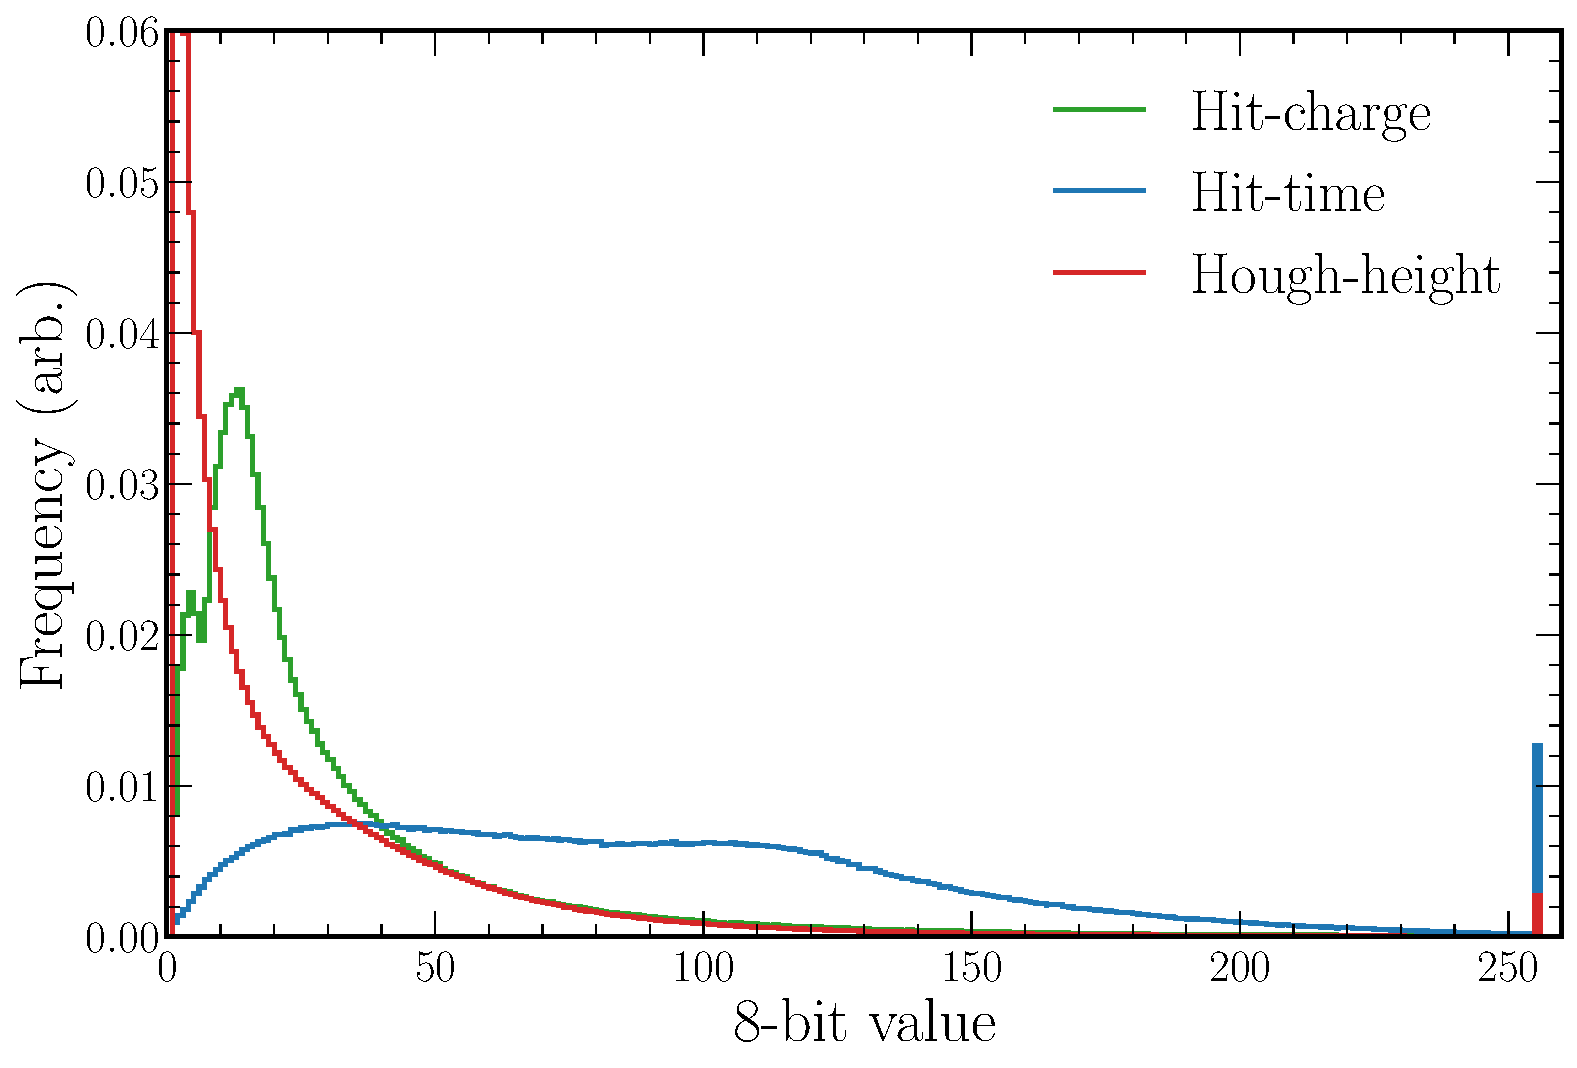
\includegraphics[width=0.7\textwidth]{diagrams/6-cvn/chipsnet/explore_8_bit_range.pdf}
    \caption[Event map encoded 8-bit distributions.]
    {The distribution of encoded 8-bit values for the hit-charge, hit-time and hough-height event
        maps. Note the maximum (\emph{capped}) bin at an 8-bit value of 255.}
    \label{fig:explore_8_bit_range}
\end{figure}

All three event maps for example events generated using the above procedure are shown in
Fig.~\ref{fig:explore_nuel_ccres_event} for a CC resonant $\nu_{e}$ event, in
Fig.~\ref{fig:explore_numu_ccdis_event} for a CC DIS $\nu_{\mu}$ event, in
Fig.~\ref{fig:explore_nuel_ncdis_event} for a NC DIS event, and in
Fig.~\ref{fig:explore_cosmic_event} for a cosmic muon event.

\begin{figure} % NUEL EVENT DIAGRAM %
    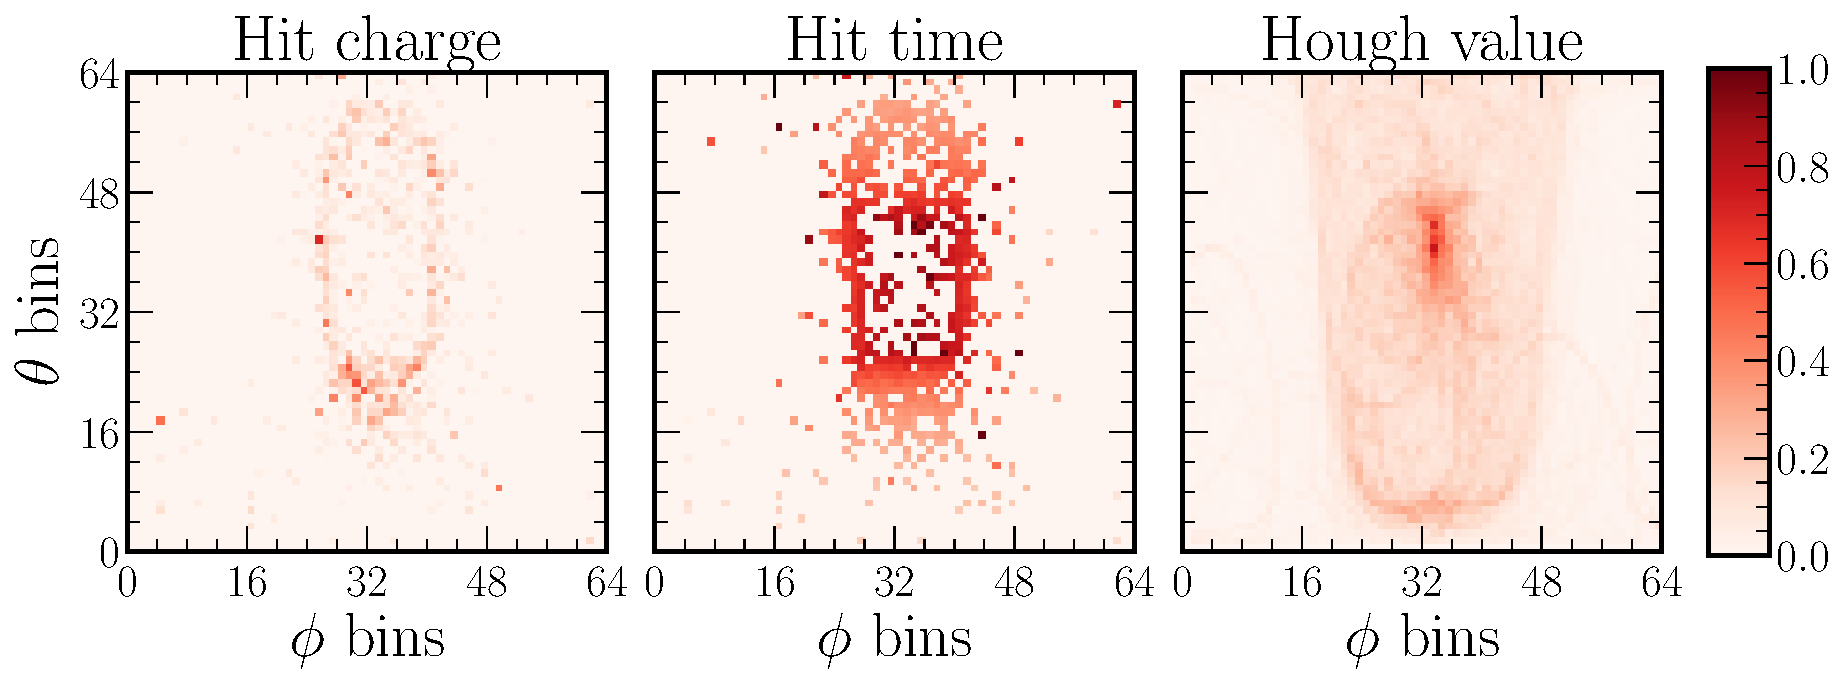
\includegraphics[width=\textwidth]{diagrams/6-cvn/chipsnet/explore_nuel_ccres_event.pdf}
    \caption[Example of a CC resonant $\nu_{e}$ event.]
    {Three channel representation of a CC resonant $\nu_{e}$ event. Initiated by a $\nu_{e}$ of
        energy \unit{3.3}{\GeV} the final state particles above the Cherenkov threshold include a
        $e^{-}$ of energy \unit{2.8}{\GeV} and a \unit{0.3}{\GeV} $\pi^{0}$.}
    \label{fig:explore_nuel_ccres_event}
\end{figure}

\begin{figure} % NUMU EVENT DIAGRAM %
    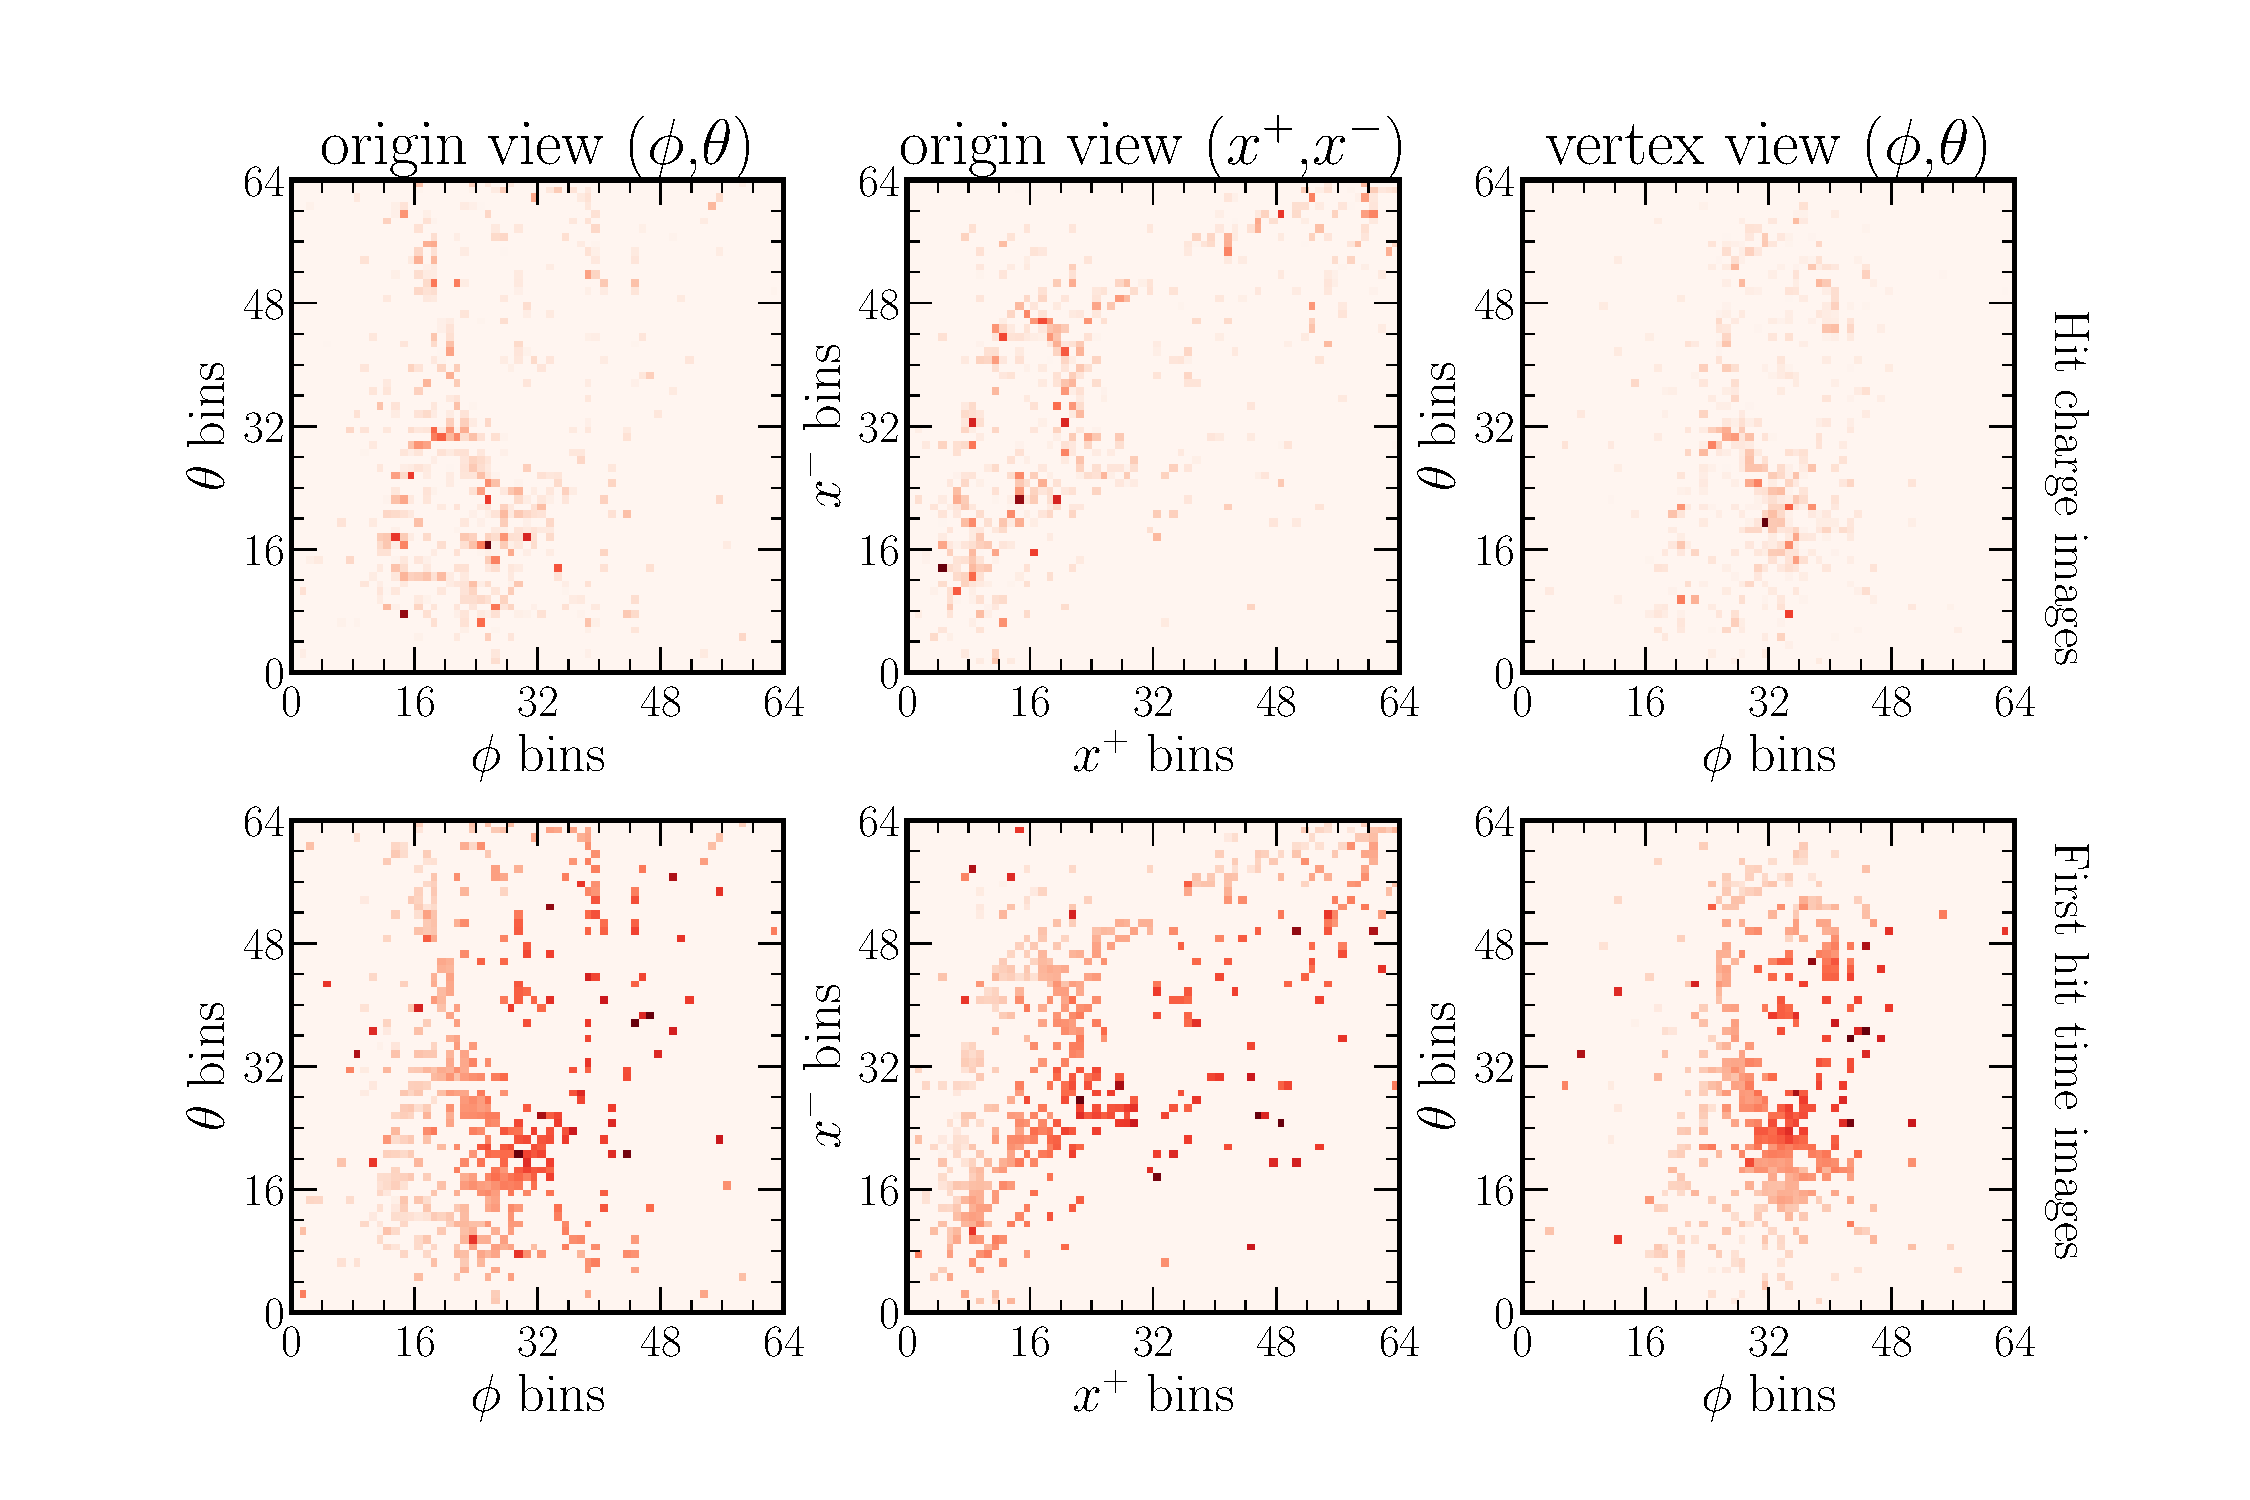
\includegraphics[width=\textwidth]{diagrams/6-cvn/chipsnet/explore_numu_ccdis_event.pdf}
    \caption[Example of a CC DIS $\nu_{\mu}$ event.]
    {Three channel representation of a CC DIS $\nu_{\mu}$ event. Initiated by a $\nu_{\mu}$ of
        energy \unit{3.5}{\GeV} the final state particles above the Cherenkov threshold include a
        $\mu^{-}$ of energy \unit{1.9}{\GeV}, a proton of energy\unit{2.0}{\GeV}, and a
        \unit{0.2}{\GeV} $\pi^{-}$.}
    \label{fig:explore_numu_ccdis_event}
\end{figure}

\begin{figure} % NC EVENT DIAGRAM %
    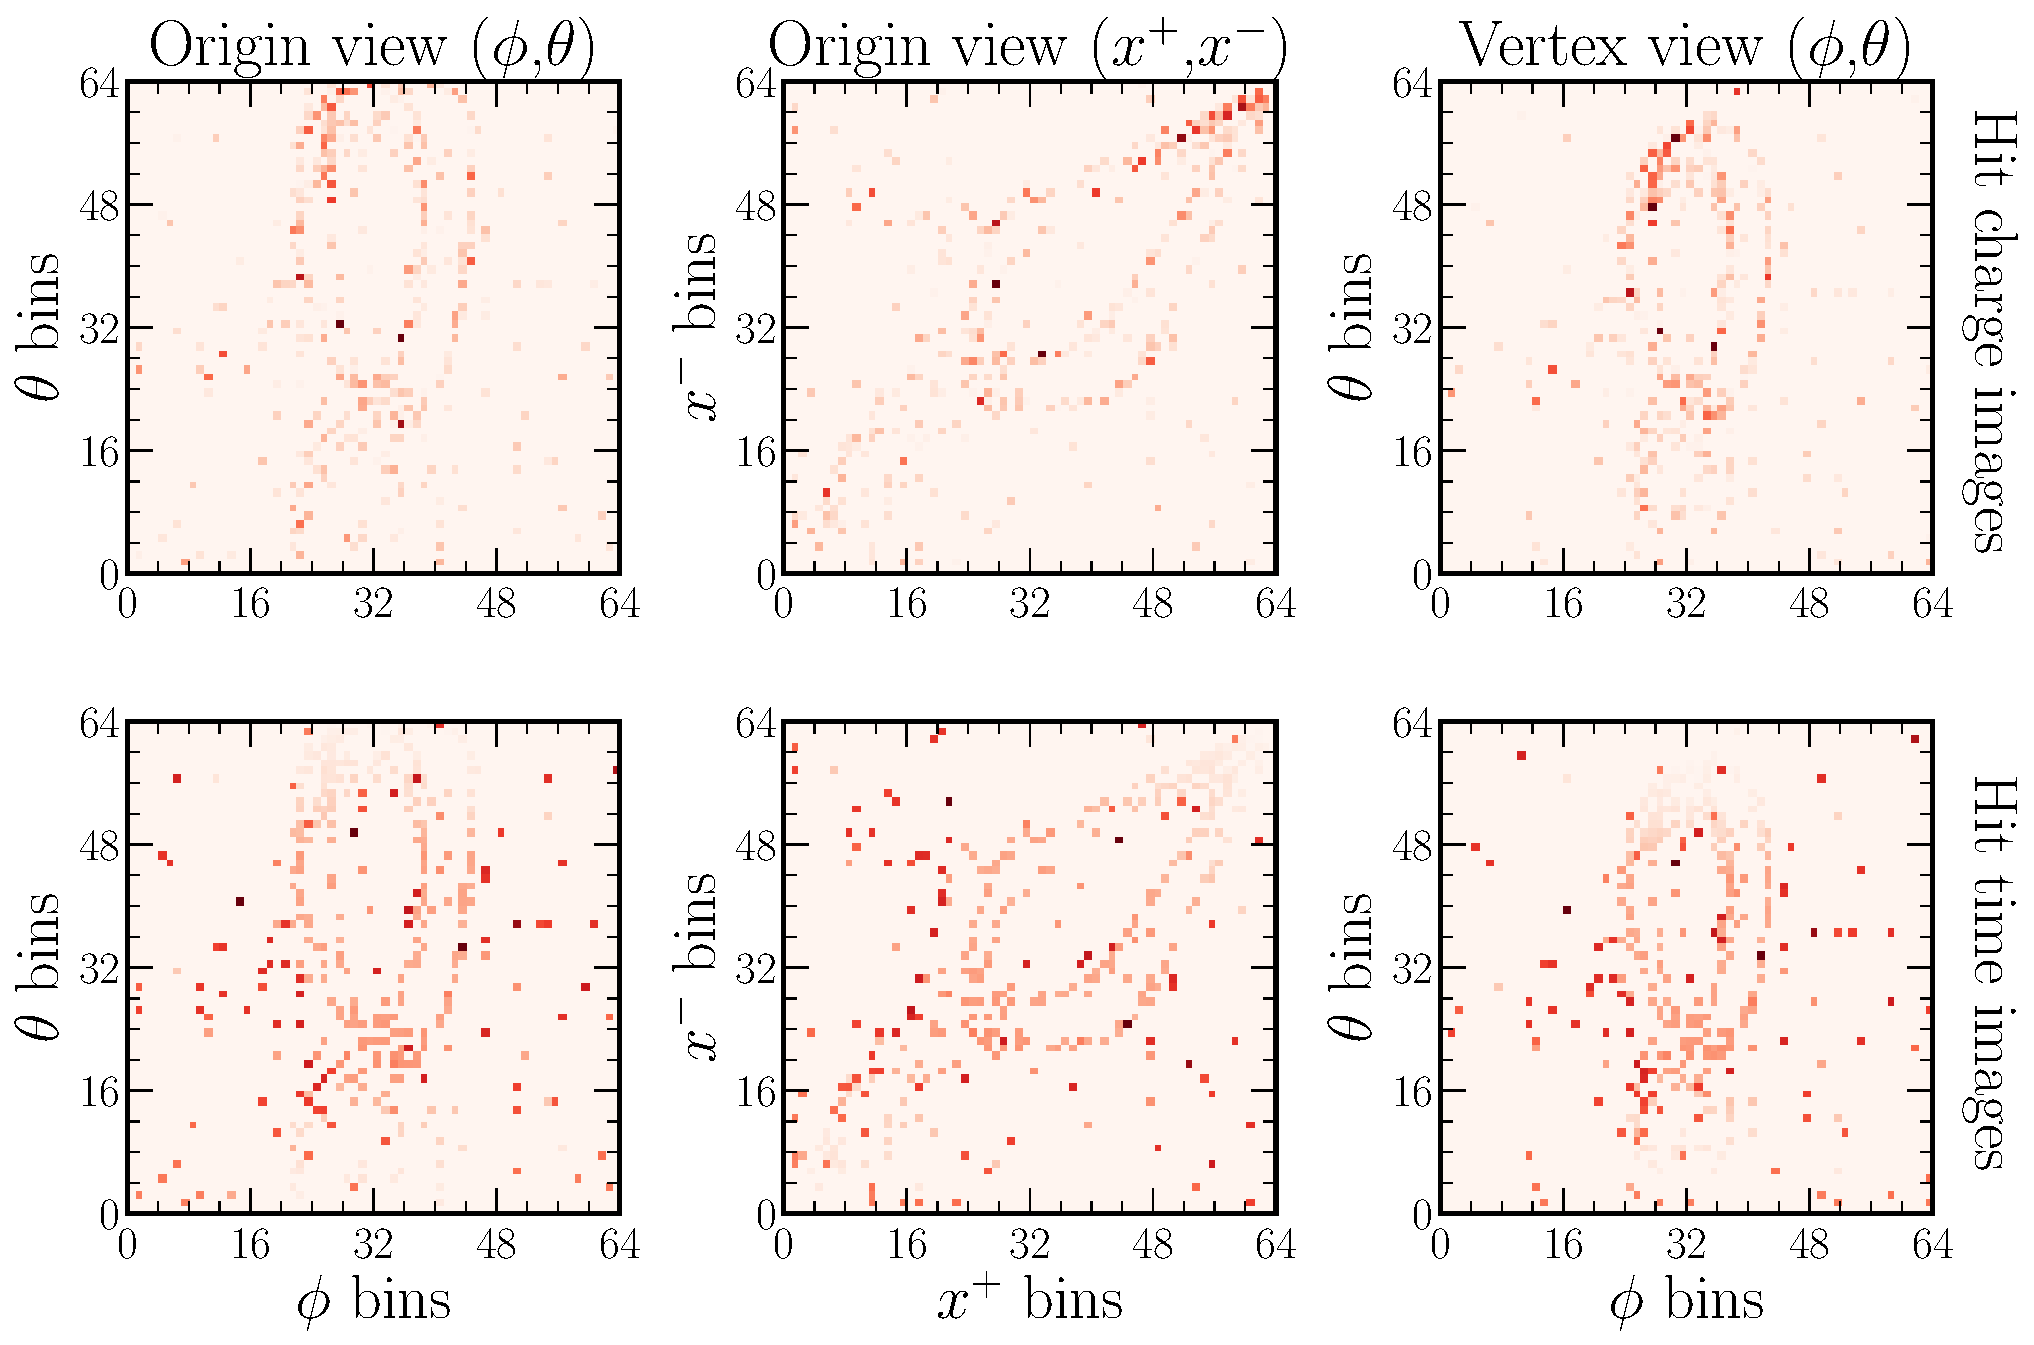
\includegraphics[width=\textwidth]{diagrams/6-cvn/chipsnet/explore_nuel_ncdis_event.pdf}
    \caption[Example of a NC DIS event.]
    {Three channel representation of a NC DIS event. Initiated by a $\nu_{e}$ of energy
        \unit{9.3}{GeV} the final state particles above the Cherenkov threshold include a proton
        of energy \unit{2.6}{\GeV} and a \unit{2.5}{\GeV} $\pi^{-}$.}
    \label{fig:explore_nuel_ncdis_event}
\end{figure}

\begin{figure} % COSMIC MUON EVENT DIAGRAM %
    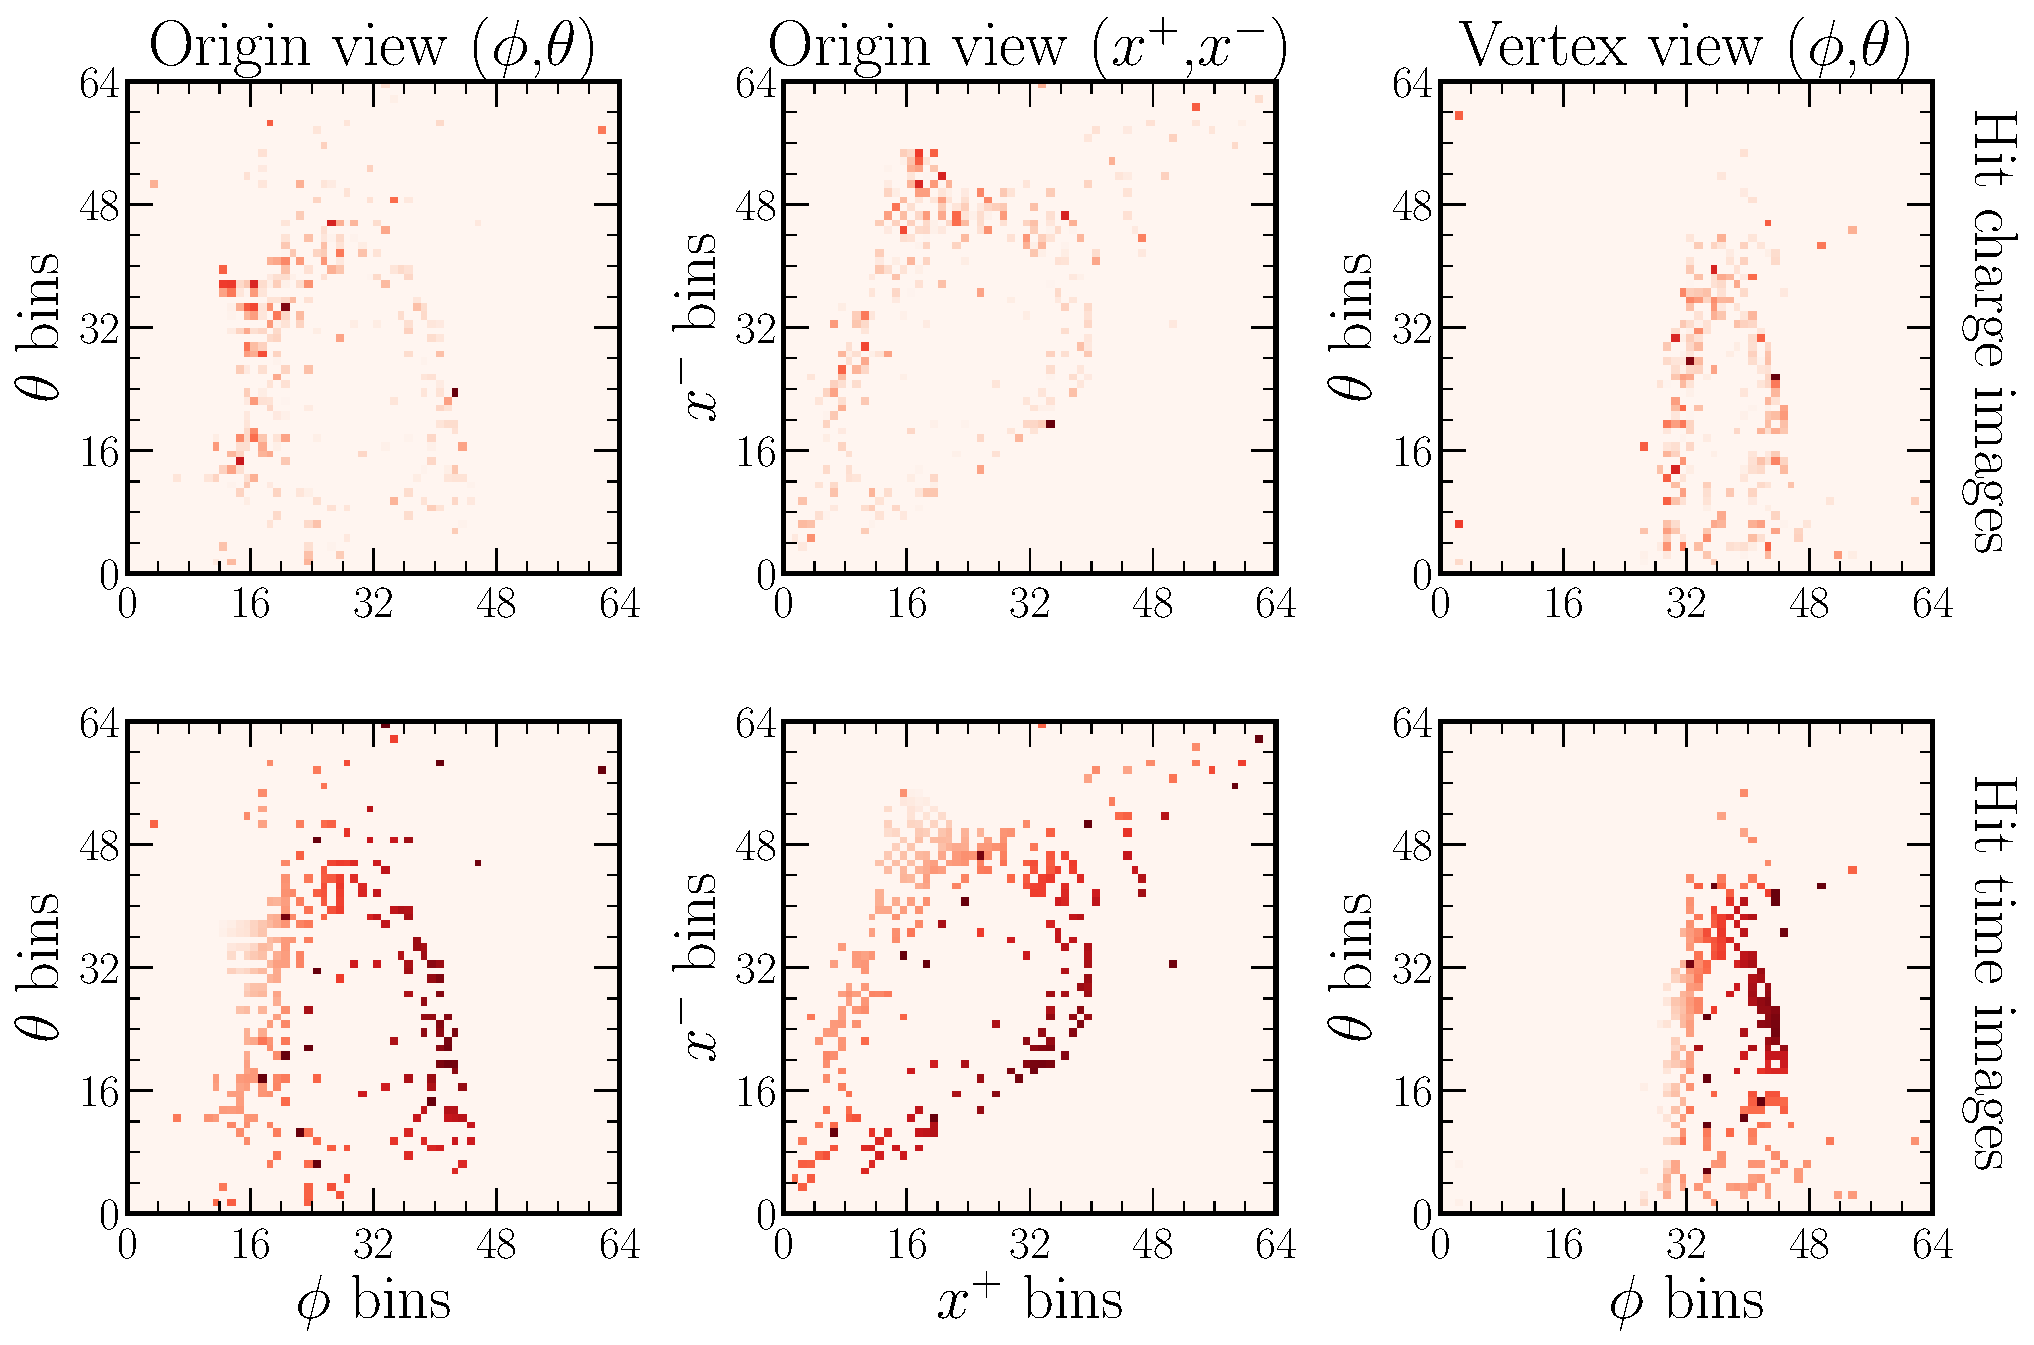
\includegraphics[width=\textwidth]{diagrams/6-cvn/chipsnet/explore_cosmic_event.pdf}
    \caption[Example of a cosmic muon event.]
    {Three channel representation of a cosmic muon event, containing a $\mu^{-}$ of energy
        \unit{2.9}{\GeV}.}
    \label{fig:explore_cosmic_event}
\end{figure}

\subsection{Baseline architecture} %%%%%%%%%%%%%%%%%%%%%%%%%%%%%%%%%%%%%%%%%%%%%%%%%%%%%%%%%%%%%%%
\label{sec:cvn_baseline_arch} %%%%%%%%%%%%%%%%%%%%%%%%%%%%%%%%%%%%%%%%%%%%%%%%%%%%%%%%%%%%%%%%%%%%

An illustrative diagram of the baseline network architecture is shown in Fig.~\ref{fig:chipsnet}.
Based on the VGG network (16 layer variant) previously mentioned in
Section.~\ref{sec:cvn_previous} and detailed in Ref.~\cite{simonyan2014} there are a few key
differences from the literature defined network, discussed below.

\begin{figure} % CHIPSNET DIAGRAM %
    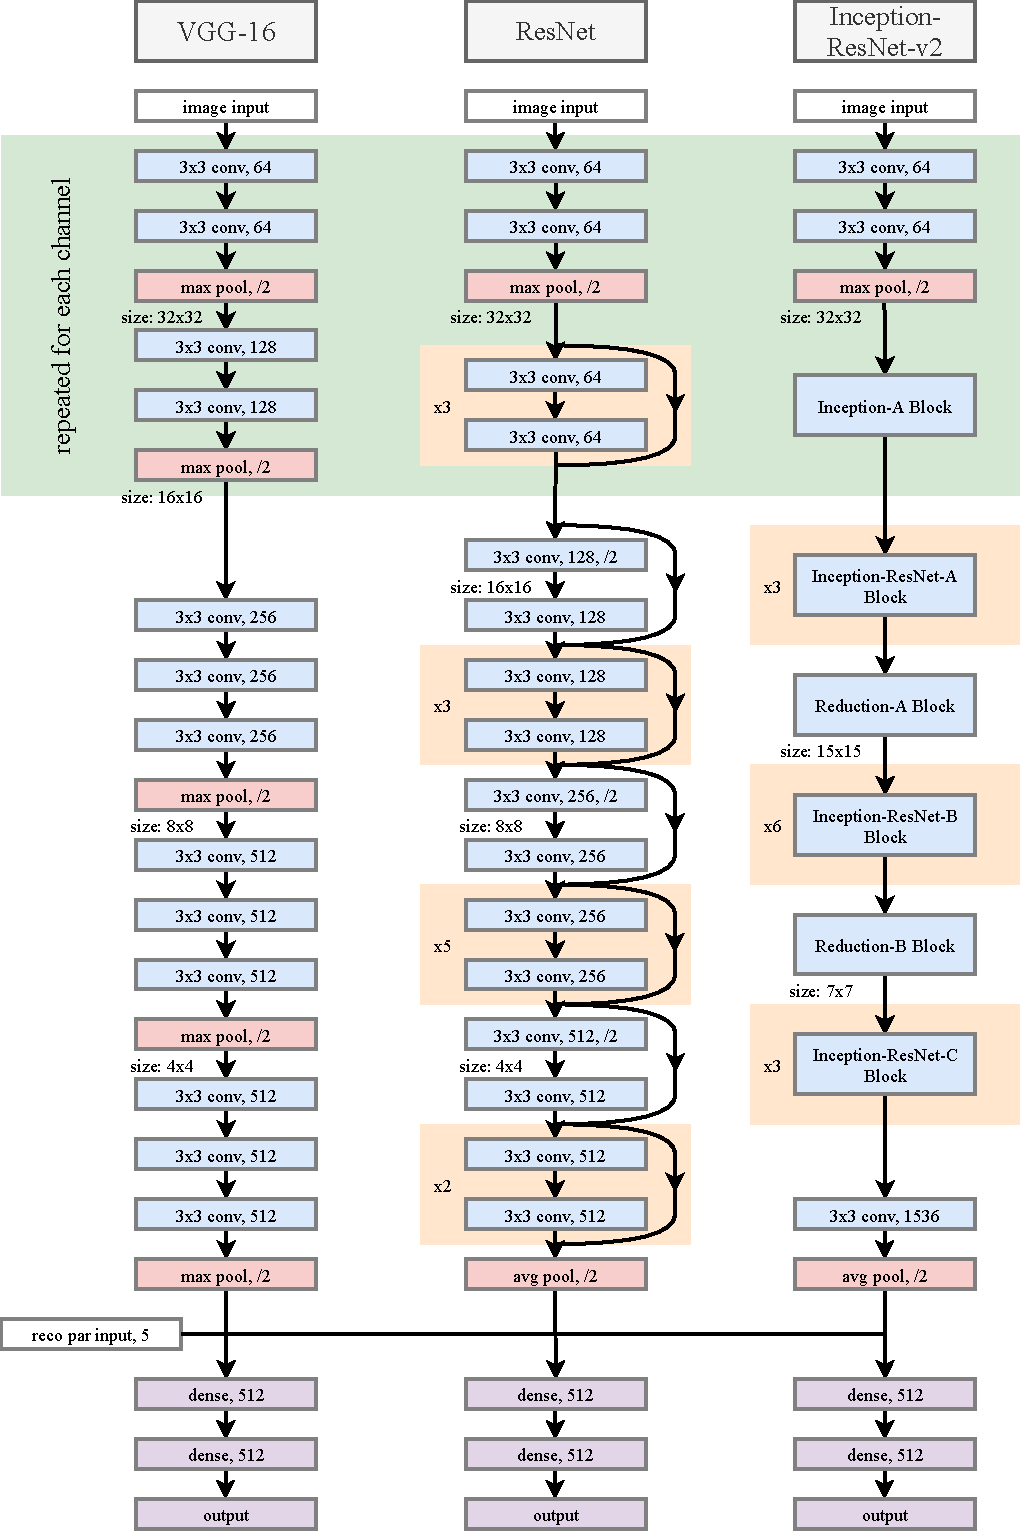
\includegraphics[width=0.7\textwidth]{diagrams/6-cvn/chipsnet.pdf}
    \caption[chipsnet short]
    {Illustrative diagram of the baseline chipsnet architecture. The three input event maps are
        separately passed through two VGG blocks each before their outputs are combined and passed
        through a further three VGG blocks. Both the number of convolutional units and kernels is
        shown for each block. The detailed block structure is shown within the grey box. The
        circular yellow $R$ and $Bn$ indicate the use of the ReLU activation function and batch
        normalisation, respectively. The flattened VGG blocks outputs are then concatenated with
        five seed parameters (seed pars) and passed through two fully-connected (FC) layers of 512
        neurons each before the output layer.}
    \label{fig:chipsnet}
\end{figure}

\begin{itemize}
    \item Each of the three event maps: hit-charge, hit-time, and hough-height are initially fed
          into three separate branches. Each branch contains two VGG blocks with two convolutional
          layers (four convolutional layers in total). The outputs from all branches are merged
          together using a concatenation layer before being fed to the rest of the network. This
          structure allows for features from each event map to be learnt independently before the
          rest of the network learns combined features.

    \item Batch normalisation as described in Section.~\ref{sec:cvn_theory_reg} is included before
          the activation (ReLU) function for every convolutional layer.

    \item Squeeze-and-excitation units as detailed in Ref.~\cite{hu2018} are included after the
          max-pooling operation in all VGG blocks. These units introduce extra parameters to model
          the interdependencies between output feature maps, allowing the network to weight each
          feature map effectively.

    \item Dropout is included at the end of each VGG block as well as after the final
          fully-connected layer. Instead of dropping individual kernel elements, the dropout
          within the blocks drops entire kernels at each training iteration, this is called
          \emph{two-dimensional spatial dropout}. The dropout after the fully-connected layers is
          normal, in that it drops out individual fully-connected neurons.

    \item Five seed parameters are concatenated with the flattened layer before the
          fully-connected layers. These are the three components of the estimated interaction
          vertex position and the two components of the estimated track direction ($s_{x},s_{y},
              s_{z},s_{\theta},s_{\phi}$). By providing the network with spatial context as to where
          in the detector the input event maps have been generated and the dominant activity
          direction,
\end{itemize}

Within chipsnet the network architecture is implemented using the Keras~\cite{chollet2015} API
built into Tensorflow. This allows for predefined common layers such as a two-dimensional
convolution or a max-pooling layer to be easily structured into a full network definition.

\subsection{Baseline outputs} %%%%%%%%%%%%%%%%%%%%%%%%%%%%%%%%%%%%%%%%%%%%%%%%%%%%%%%%%%%%%%%%%%%%
\label{sec:cvn_baseline_outputs} %%%%%%%%%%%%%%%%%%%%%%%%%%%%%%%%%%%%%%%%%%%%%%%%%%%%%%%%%%%%%%%%%

Many CNN applications are found to benefit from learning multiple tasks at the same time, using
the same inputs. This is believed to be the case as training with multiple tasks tends to return a
network with an improved generalised representation of the inputs. Thus, features learnt for one
task can improve the performance of another. Additionally, multiple tasks work to regularise any
one output from overfitting. Commonly named \emph{multi-task} learning, this methodology is used
extensively in this work.

In order to train a network with multiple tasks (outputs), a loss function $E_{tot}$ must be
defined to combine the individual loss functions for each task $E_{i}$. The simplest way to do
this is via a linear weighted sum, such that
\begin{equation}
    E_{tot} = \sum_{i=1}^{i=N}w_{i}E_{i},
    \label{eq:multi_simple}
\end{equation}
where $N$ is the number of tasks and $w_{i}$ are the associated weights. In this work this is
referred to as the \emph{simple} multi-task loss.

The final network performance can strongly depend on the relative weighting between loss
functions, especially when the values returned from the different loss function differ by many
order of magnitude. Therefore, finding the optimal $w_{i}$ weights can be both difficult and
time-consuming. Another approach outlined in Ref.~\cite{kendall2018} aims to remedy this problem
by learning the optimal weighting between loss functions. This is done by introducing an
additional trainable parameter $\sigma_{i}$, for each loss function, such that
\begin{equation}
    E_{tot}= \sum_{i=1}^{i=N}\frac{1}{2\sigma_{i}^2}E_{i}+ \log\sigma_{i}.
    \label{eq:multi_learnt}
\end{equation}
In this work we refer to this as the \emph{learnt} multi-task loss.

The specific number and nature of outputs for the different networks are detailed in
Section.~\ref{sec:cvn_specific}. Although physically motivated to some degree, the exact set of
tasks and the loss combination technique used is mainly driven by trial-and-error. The chipsnet
software is specifically designed to enable this process by making it easy to configure the
network outputs via a simple configuration file.

\subsection{Baseline Training} %%%%%%%%%%%%%%%%%%%%%%%%%%%%%%%%%%%%%%%%%%%%%%%%%%%%%%%%%%%%%%%%%%%
\label{sec:cvn_baseline_training} %%%%%%%%%%%%%%%%%%%%%%%%%%%%%%%%%%%%%%%%%%%%%%%%%%%%%%%%%%%%%%%%

All three networks are trained using Tensorflow 2.3.0 on an 18 core CPU (36 thread) machine
equipped with four NVIDIA GeForce RTX 2080 graphics processing units (GPUs). The Tensorflow
dataset API is used to create an efficient input data pipeline where data is loaded on-the-fly at
training time. This ensures all GPU threads are utilised loading, decoding, and preprocessing data
for the primary GPU based calculations before being needed, maximising computational efficiency.

During preprocessing, all 8-bit input map values are converted to 32-bit float values bounded
between zero and one. Additionally, a random factor scaling is applied to each map bin. Generated
from a Gaussian centred on one with a standard deviation of $\sigma_{r}$, by fluctuating the bin
values in this way the network is forced to focus less on the absolute bin values and more on the
underlying event topology. Furthermore, this provides valuable regularisation to reduce
overfitting.

A minibatch training strategy of minibatch size of $n_{b}$, using the Adam
optimiser~\cite{kingma2014} with $\beta_{1}=0.9$, $\beta_{2}=0.999$, and $\epsilon = 1e-7$ is
used. The exact training sample sizes are given in Section.~\ref{sec:cvn_specific} but for all
networks a 95\% training to 5\% validation data split is employed allowing for the implementation
of early stopping. The learning rate for each epoch $\eta_{e}$ is set to decrease throughout
training according to
\begin{equation}
    \eta_{e}=\frac{\eta_{0}}{1+c_{d}(e-1)},
\end{equation}
where $\eta_{0}$ is the initial learning rate, $e$ is the epoch number (starting at one), and
$c_{d}$ is the learning rate decay coefficient.

The list below details all the possible \emph{hyperparameters} that are tunable when training each
network. All are optimised for each specific network using the SHERPA hyperparameter tuning
framework~\cite{hertel2020}. Random configurations selected from either a range or selection of
choices for each hyperparameter (also outlined below) are tested to maximise performance.

\begin{itemize}
    \item \textbf{Initial learning rate, $\eta_{0}$:} in a range from 0.00005 to 0.001.
    \item \textbf{Learning rate decay coefficient, $c_{d}$:} in a range from 0.2 to 0.8.
    \item \textbf{Dropout probability, $p_{d}$:} in a range from 0.0 to 0.5.
    \item \textbf{Random scaling size, $\sigma_{r}$:} in a range from 0.0 to 0.1.
    \item \textbf{Minibatch size, $n_{b}$:} choosing from 32, 64, 128, or 256.
    \item \textbf{Multi-task loss combination strategy:} choosing from \emph{simple} or
          \emph{learnt}.
\end{itemize}

\section{Specific implementations} %%%%%%%%%%%%%%%%%%%%%%%%%%%%%%%%%%%%%%%%%%%%%%%%%%%%%%%%%%%%%%%
\label{sec:cvn_specific} %%%%%%%%%%%%%%%%%%%%%%%%%%%%%%%%%%%%%%%%%%%%%%%%%%%%%%%%%%%%%%%%%%%%%%%%%

The specific CNN implementations for cosmic rejection, beam classification and energy estimation
are outlined below. It is important to note that the exact configuration of networks outlined here
is the result of extensive testing designed to maximise the selection of a pure and efficient
sample of $\nu_{e}$ beam events whose neutrino energy can also be accurately determined.

For example, if cosmic and beam classification are combined into a single network, both objectives
see a reduction in performance. The same is also true if either classification task and neutrino
energy estimation are combined. However, specific secondary outputs such as counting the number of
primary particles in conjunction with beam classification are seen to improve performance. It is
clear, therefore, that the multi-task approach only works for tasks that require a similar
representation of the inputs to be learnt by the network. Put simply; the tasks must be similar.

\subsection{Cosmic rejection} %%%%%%%%%%%%%%%%%%%%%%%%%%%%%%%%%%%%%%%%%%%%%%%%%%%%%%%%%%%%%%%
\label{sec:cvn_specific_cosmic} %%%%%%%%%%%%%%%%%%%%%%%%%%%%%%%%%%%%%%%%%%%%%%%%%%%%%%%%%%%%%%%%%%

The cosmic rejection network aims to prevent the large expected cosmic muon background from
contaminating the final selected sample of beam events. Therefore, the primary task is a simple
binary classification between beam and cosmic events. Additionally, training the network to also
separate events where the primary charged lepton escapes the detector volume or not, is found to
improve cosmic rejection performance. As a large proportion of cosmic muons are relatively high in
energy and, therefore, escape the detector in this fashion, there is motivation as to why this
additional task is helpful.

The network is trained on a sample of 3.15 million simulated events, roughly $1/3^{rd}$
$\nu_{\mu}$ beam events, $1/3^{rd}$ $\nu_{e}$ beam events, and $1/3^{rd}$ cosmic muon events. The
counts of which are shown in Fig.~\ref{fig:cosmic_training_sample}. All beam events (both
$\nu_{\mu}$ and $\nu_{e}$) are generated using the expected \chips $\nu_{\mu}$ energy spectrum to
closely mimic the dominant $\nu_{\mu}$ beam component and appeared $\nu_{e}$ signal. The full
sample is split 95\% to 5\% for training and validation, respectively.

\begin{figure} % COSMIC TRAINING SAMPLE DIAGRAM %
    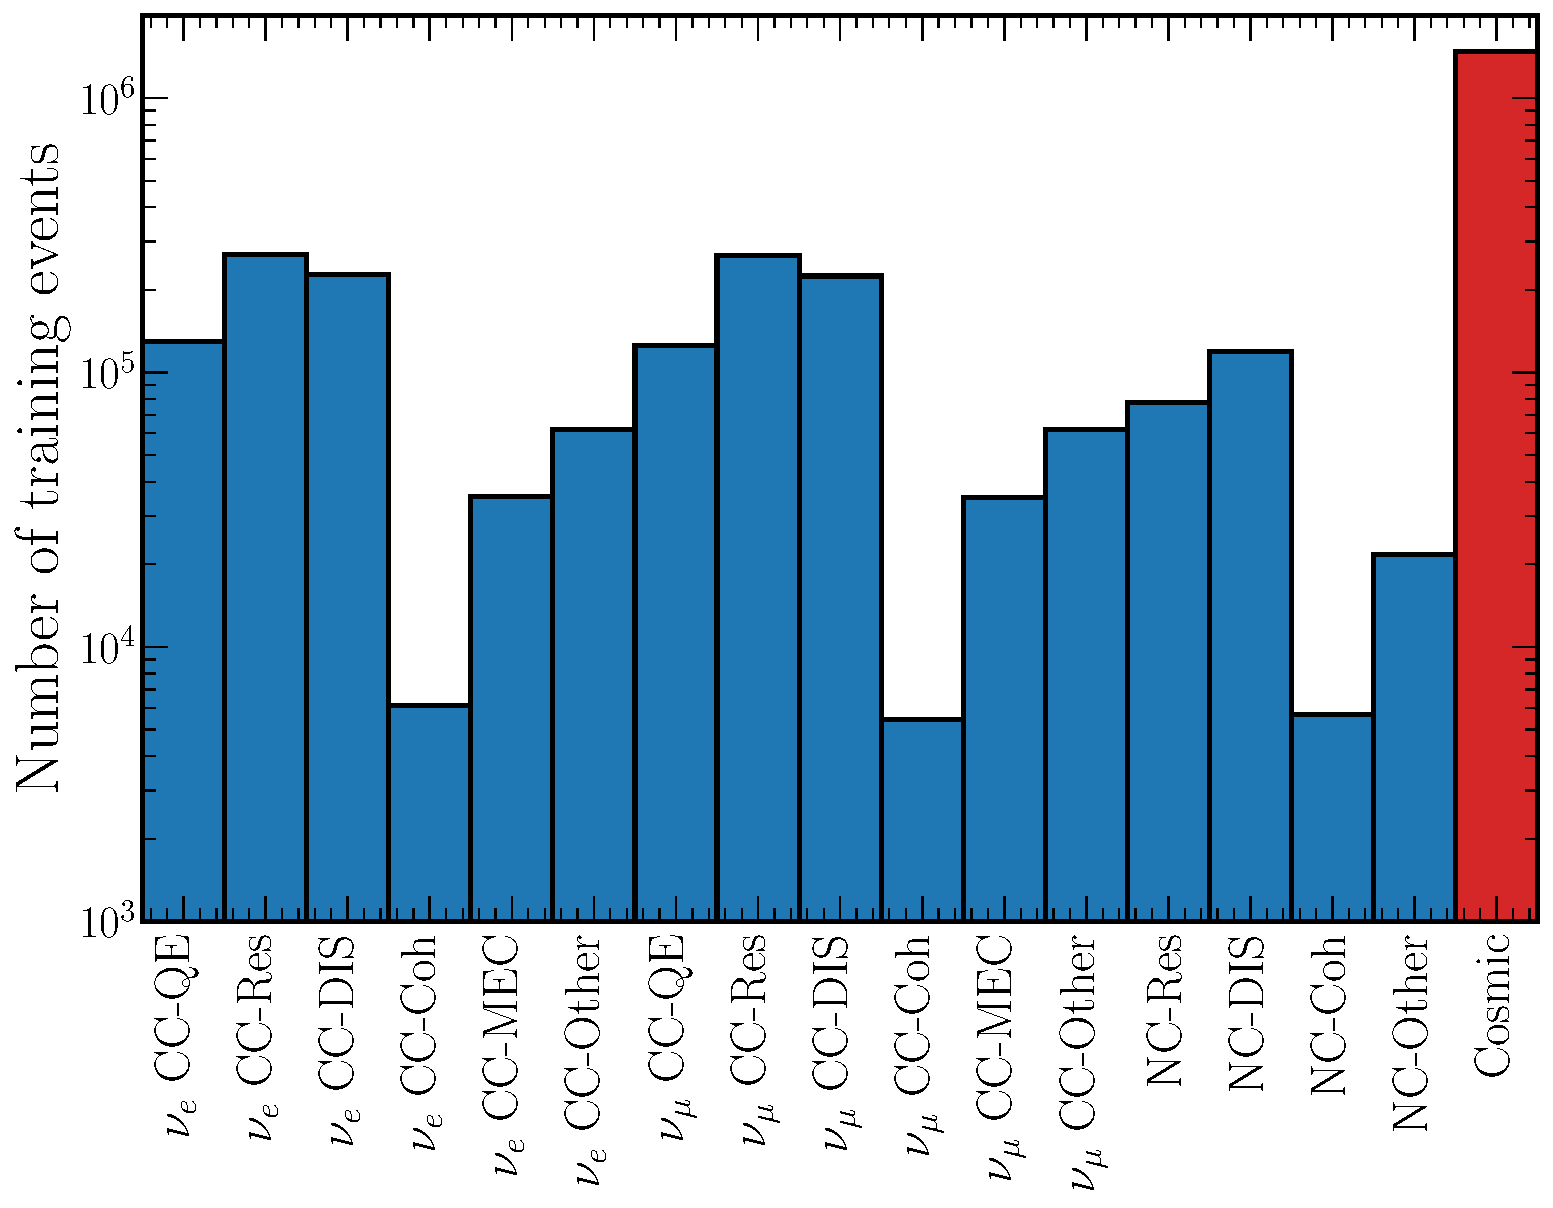
\includegraphics[width=0.7\textwidth]{diagrams/6-cvn/chipsnet/explore_cosmic_training_sample.pdf}
    \caption[Number of training events per category for the cosmic rejection network.]
    {Number of training events per category for the cosmic rejection network. All beam event
        interaction types are shown, however, all are classed as beam events (blue) in training
        against cosmic events (red).}
    \label{fig:cosmic_training_sample}
\end{figure}

There are two outputs to the cosmic rejection network:
\begin{enumerate}
    \item \textbf{Cosmic score (1 neuron):} Returns a score between zero and one corresponding to
          whether the event is beam or cosmic like. The binary cross-entropy loss function in
          Eq.~\ref{eq:binary_cross_entropy} is used for training with a simple multi-task weight
          of $1$.
    \item \textbf{Escapes score (1 neuron):} Returns a score between zero and one corresponding to
          whether the charged lepton in an event is contained or escapes the detector. The binary
          cross-entropy loss function in Eq.~\ref{eq:binary_cross_entropy} is used for training
          with a simple multi-task weight of $1$. NC beam events without a charged lepton are
          masked (do not contribute to the loss) during training for this output.
\end{enumerate}

The network is allowed to train for up to 30 epochs using the SHERPA optimised hyperparameters:
$\eta_{0}=0.00005$, $c_{d}=0.7$, $p_{d}=0.1$, $\sigma_{r}=0.02$, and $n_{b}=128$, with a simple
multi-task loss combination as given in Eq.~\ref{eq:multi_simple}. Typically, only 6 epochs are
required to reach the maximum validation sample `cosmic score' accuracy, with early stopping
halting training after 11 epochs, as can be seen in Fig.~\ref{fig:final_cosmic_history}. Training
takes approximately 15 hours.

\begin{figure} % COSMIC HISTORY DIAGRAM %
    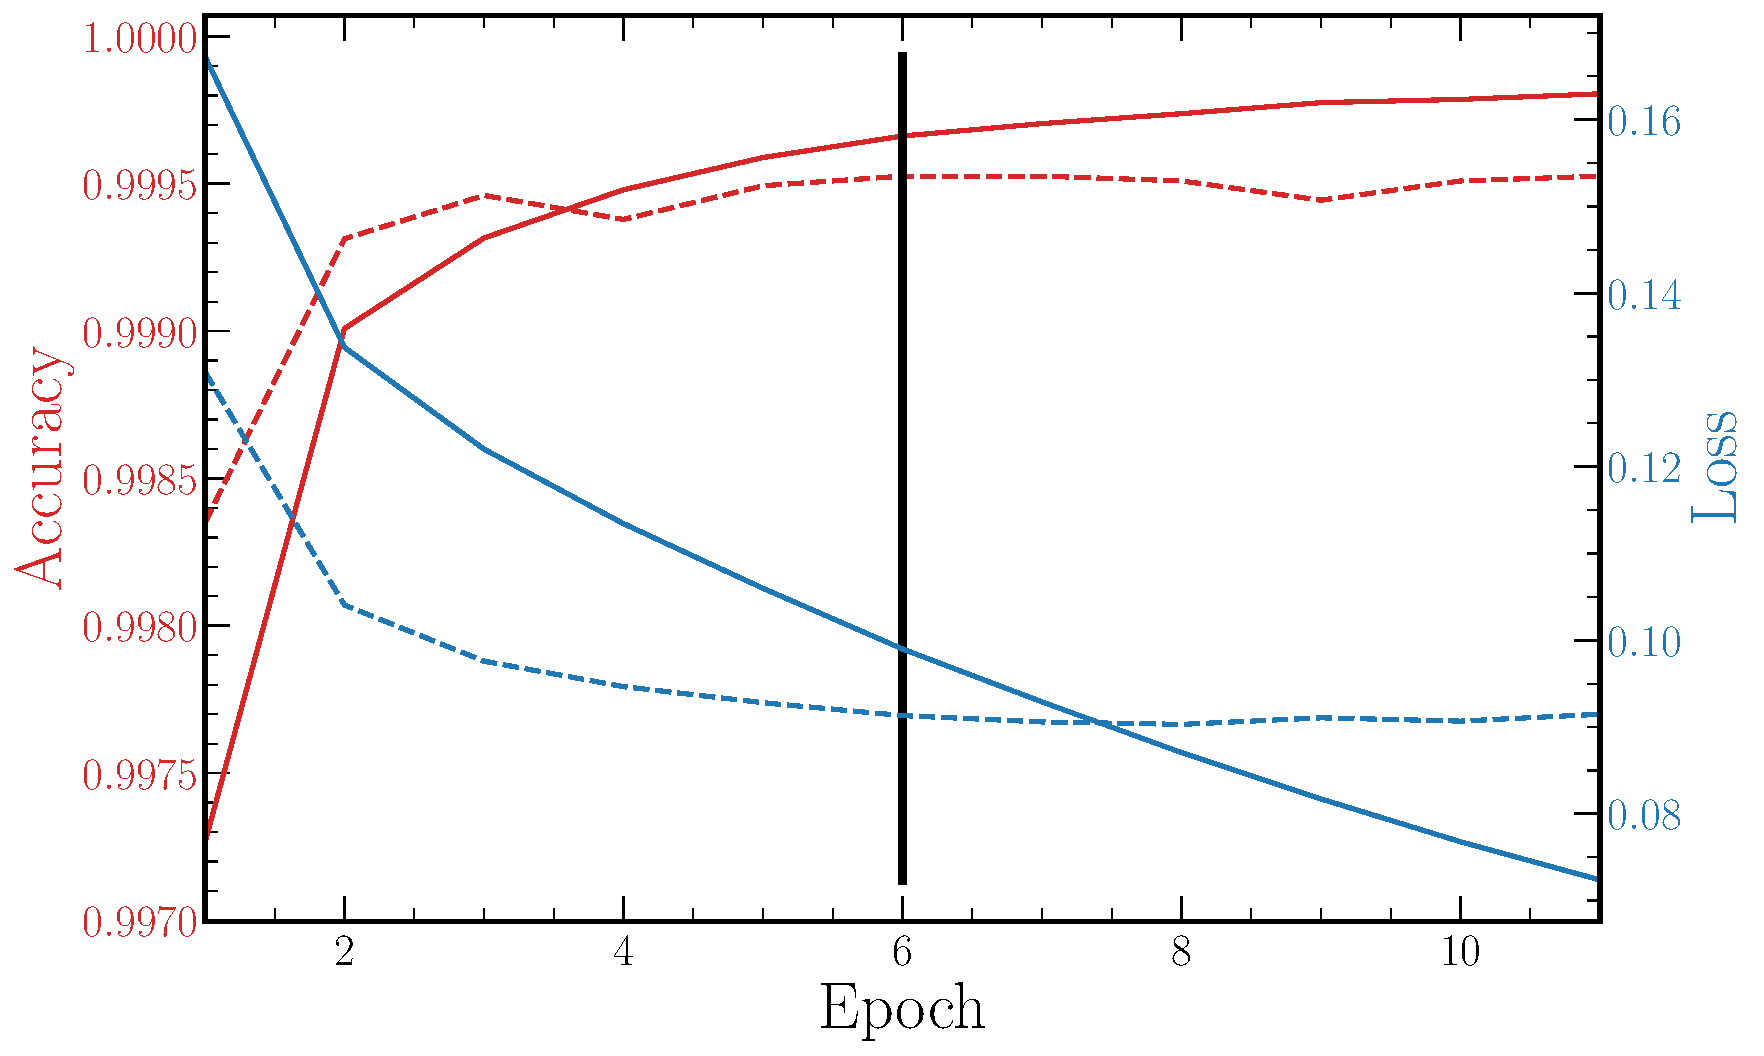
\includegraphics[width=0.7\textwidth]{diagrams/6-cvn/chipsnet/final_cosmic_history.pdf}
    \caption[Loss and accuracy throughout training for the cosmic rejection network.]
    {Total loss and `cosmic score' accuracy for both the training sample (solid) and validation
        sample (dashed) throughout training for the cosmic rejection network. The final network
        weights are taken at epoch 6 as shown by the vertical black line.}
    \label{fig:final_cosmic_history}
\end{figure}

\subsection{Beam classification}%%%%%%%%%%%%%%%%%%%%%%%%%%%%%%%%%%%%%%%%%%%%%%%%%%%%%%%%%%%%%%%%%%
\label{sec:cvn_specific_beam} %%%%%%%%%%%%%%%%%%%%%%%%%%%%%%%%%%%%%%%%%%%%%%%%%%%%%%%%%%%%%%%%%%%%

The beam classification network aims to separate beam events by their interaction type primarily
to select a pure and efficient sample of appeared $\nu_{e}$ events, but also a sample of survived
CC $\nu_{\mu}$ events. Therefore, the primary task is a categorical classification between CC
$\nu_{e}$, CC $\nu_{\mu}$, and NC events. No attempt is made to separate the appeared CC $\nu_{e}$
and intrinsic beam CC $\nu_{e}$ components as they are impossible to tell apart, except for their
energy distributions. Similar to the implementation used by DUNE~\cite{collaboration2020},
alongside the core classification additional classification and particle counting tasks outlined
below are included to improve performance.

The network is trained on a sample of 1.67 million simulated events, roughly half $\nu_{\mu}$ beam
events, and half $\nu_{e}$ beam events, as shown in Fig.~\ref{fig:beam_training_sample}. All
events (both $\nu_{\mu}$ and $\nu_{e}$) are generated using the expected \chips $\nu_{\mu}$ energy
spectrum to closely mimic the dominant $\nu_{\mu}$ beam component and appeared $\nu_{e}$ signal.
The full sample is split 95\% to 5\% for training and validation, respectively.

\begin{figure} % BEAM TRAINING SAMPLE DIAGRAM %
    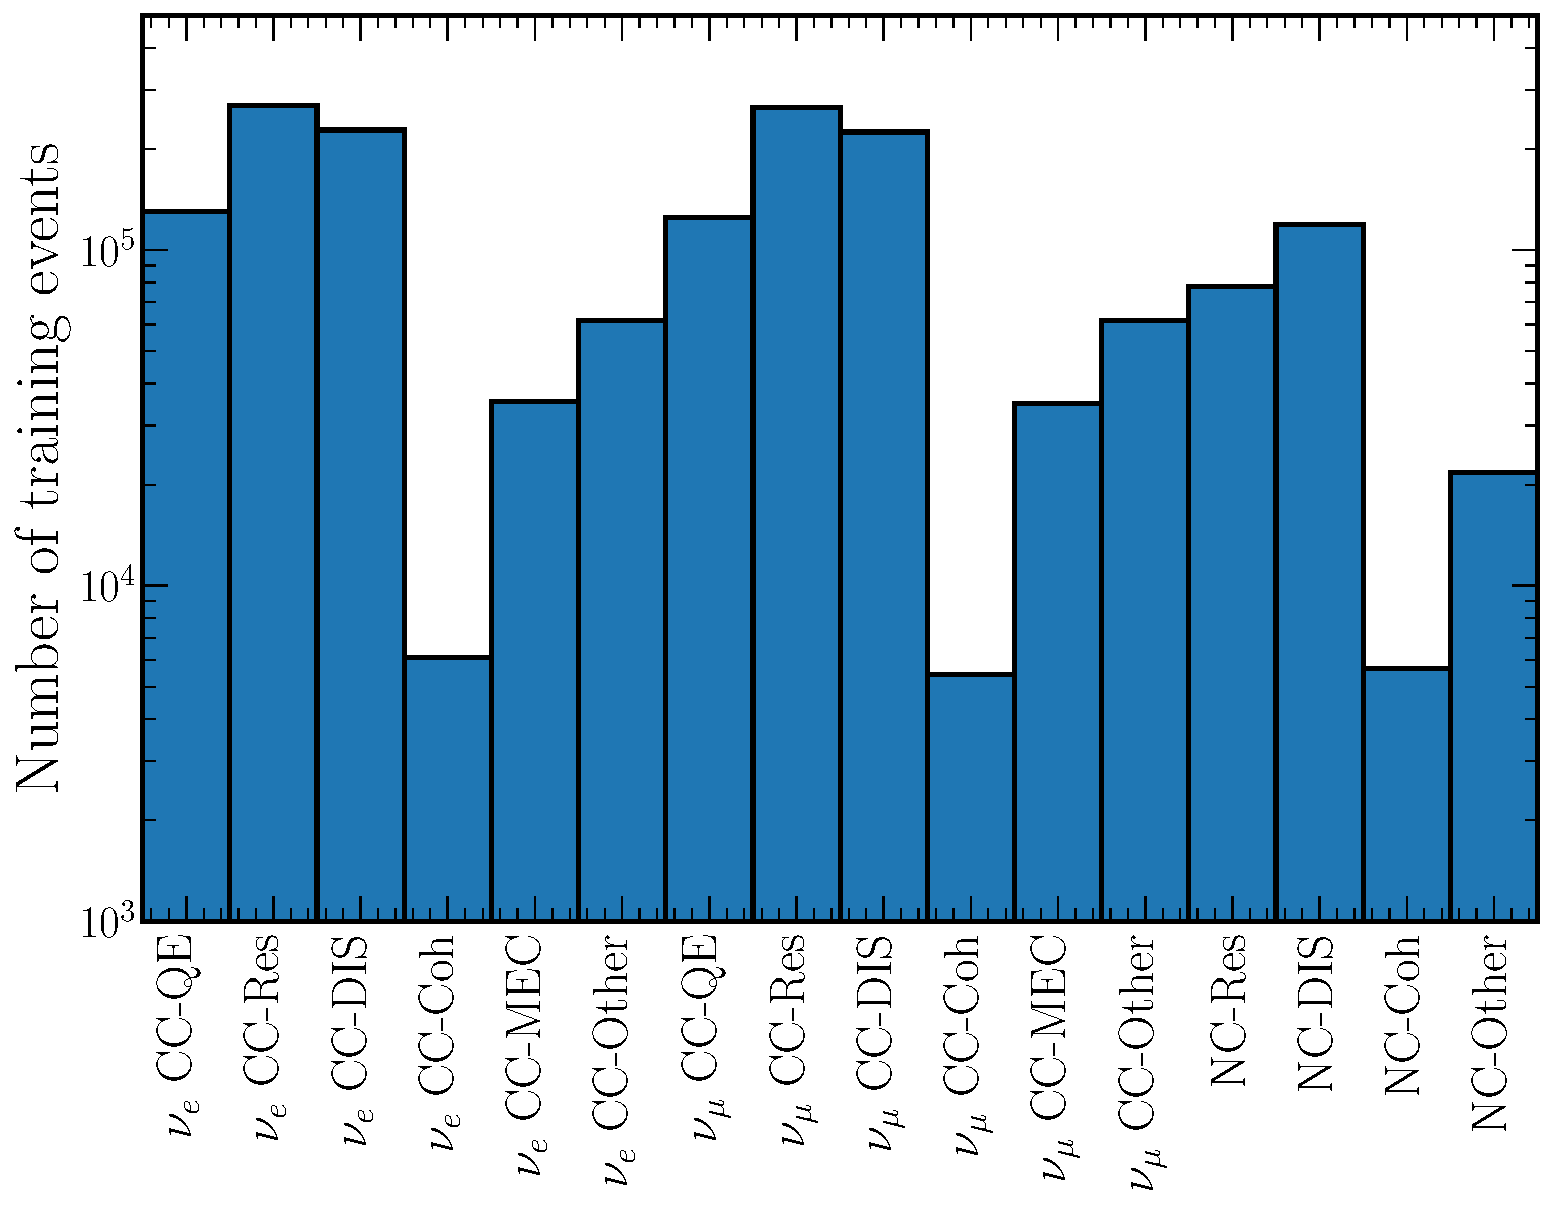
\includegraphics[width=0.7\textwidth]{diagrams/6-cvn/chipsnet/explore_beam_training_sample.pdf}
    \caption[Number of training events per category for the beam classification network.]
    {Number of training events per category for the beam classification network. All beam event
        interaction types are shown.}
    \label{fig:beam_training_sample}
\end{figure}

There are nine outputs to the beam classification network:
\begin{enumerate}
    \item \textbf{Combined category (3 neurons):} Returns a classification probability score
          between zero and one for each of CC $\nu_{e}$, CC $\nu_{\mu}$, and NC (summing to one).
          The categorical cross-entropy loss function in Eq.~\ref{eq:categorical_cross_entropy} is
          used for training with a simple multi-task weight of $1$.
    \item \textbf{CC category (6 neurons):} Returns a classification probability score between
          zero and one for each of CC-QE, CC-Res, CC-DIS, CC-Coh, CC-MEC and CC-other (summing to
          one). The categorical cross-entropy loss function in
          Eq.~\ref{eq:categorical_cross_entropy} is used for training with a simple multi-task
          weight of $1$. NC events are masked (do not contribute to the loss) during training for
          this output.
    \item \textbf{NC category (4 neurons):} Returns a classification probability score between
          zero and one for each of NC-Res, NC-DIS, NC-Coh and NC-other (summing to one). The
          categorical cross-entropy loss function in Eq.~\ref{eq:categorical_cross_entropy} is
          used for training with a simple multi-task weight of $1$. CC events are masked (do not
          contribute to the loss) during training for this output.
    \item \textbf{Electron count (4 neurons):} Returns a classification probability score between
          zero and one for each of 0, 1, 2, and 3+ electrons in the final state (summing to one).
          The categorical cross-entropy loss function in Eq.~\ref{eq:categorical_cross_entropy} is
          used for training with a simple multi-task weight of $1$.
    \item \textbf{Muon count (4 neurons):} Returns a classification probability score between zero
          and one for each of 0, 1, 2, and 3+ muons in the final state (summing to one). The
          categorical cross-entropy loss function in Eq.~\ref{eq:categorical_cross_entropy} is
          used for training with a simple multi-task weight of $1$.
    \item \textbf{Proton count (4 neurons):} Returns a classification probability score between
          zero and one for each of 0, 1, 2, and 3+ protons in the final state (summing to one).
          The categorical cross-entropy loss function in Eq.~\ref{eq:categorical_cross_entropy} is
          used for training with a simple multi-task weight of $1$.
    \item \textbf{$\pi^{\pm}$ count (4 neurons):} Returns a classification probability score
          between zero and one for each of 0, 1, 2, and 3+ charged pions in the final state
          (summing to one). The categorical cross-entropy loss function in
          Eq.~\ref{eq:categorical_cross_entropy} is used for training with a simple multi-task
          weight of $1$.
    \item \textbf{$\pi^{0}$ count (4 neurons):} Returns a classification probability score between
          zero and one for each of 0, 1, 2, and 3+ neutral pions in the final state (summing to
          one). The categorical cross-entropy loss function in
          Eq.~\ref{eq:categorical_cross_entropy} is used for training with a simple multi-task
          weight of $1$.
    \item \textbf{Photon count (4 neurons):} Returns a classification probability score between
          zero and one for each of 0, 1, 2, and 3+ photons in the final state (summing to one).
          The categorical cross-entropy loss function in Eq.~\ref{eq:categorical_cross_entropy} is
          used for training with a simple multi-task weight of $1$.
\end{enumerate}

The network is allowed to train for up to 30 epochs using the SHERPA optimised hyperparameters:
$\eta_{0}=0.0002$, $c_{d}=0.5$, $p_{d}=0.1$, $\sigma_{r}=0.02$, and $n_{b}=128$, with a simple
multi-task loss combination as given in Eq.~\ref{eq:multi_simple}. Typically, only 7 epochs are
required to reach the maximum validation sample `combined category' accuracy, with early stopping
halting training after 12 epochs, as can be seen in Fig.~\ref{fig:final_beam_history}. Training
takes approximately 15 hours.

\begin{figure} % BEAM HISTORY DIAGRAM %
    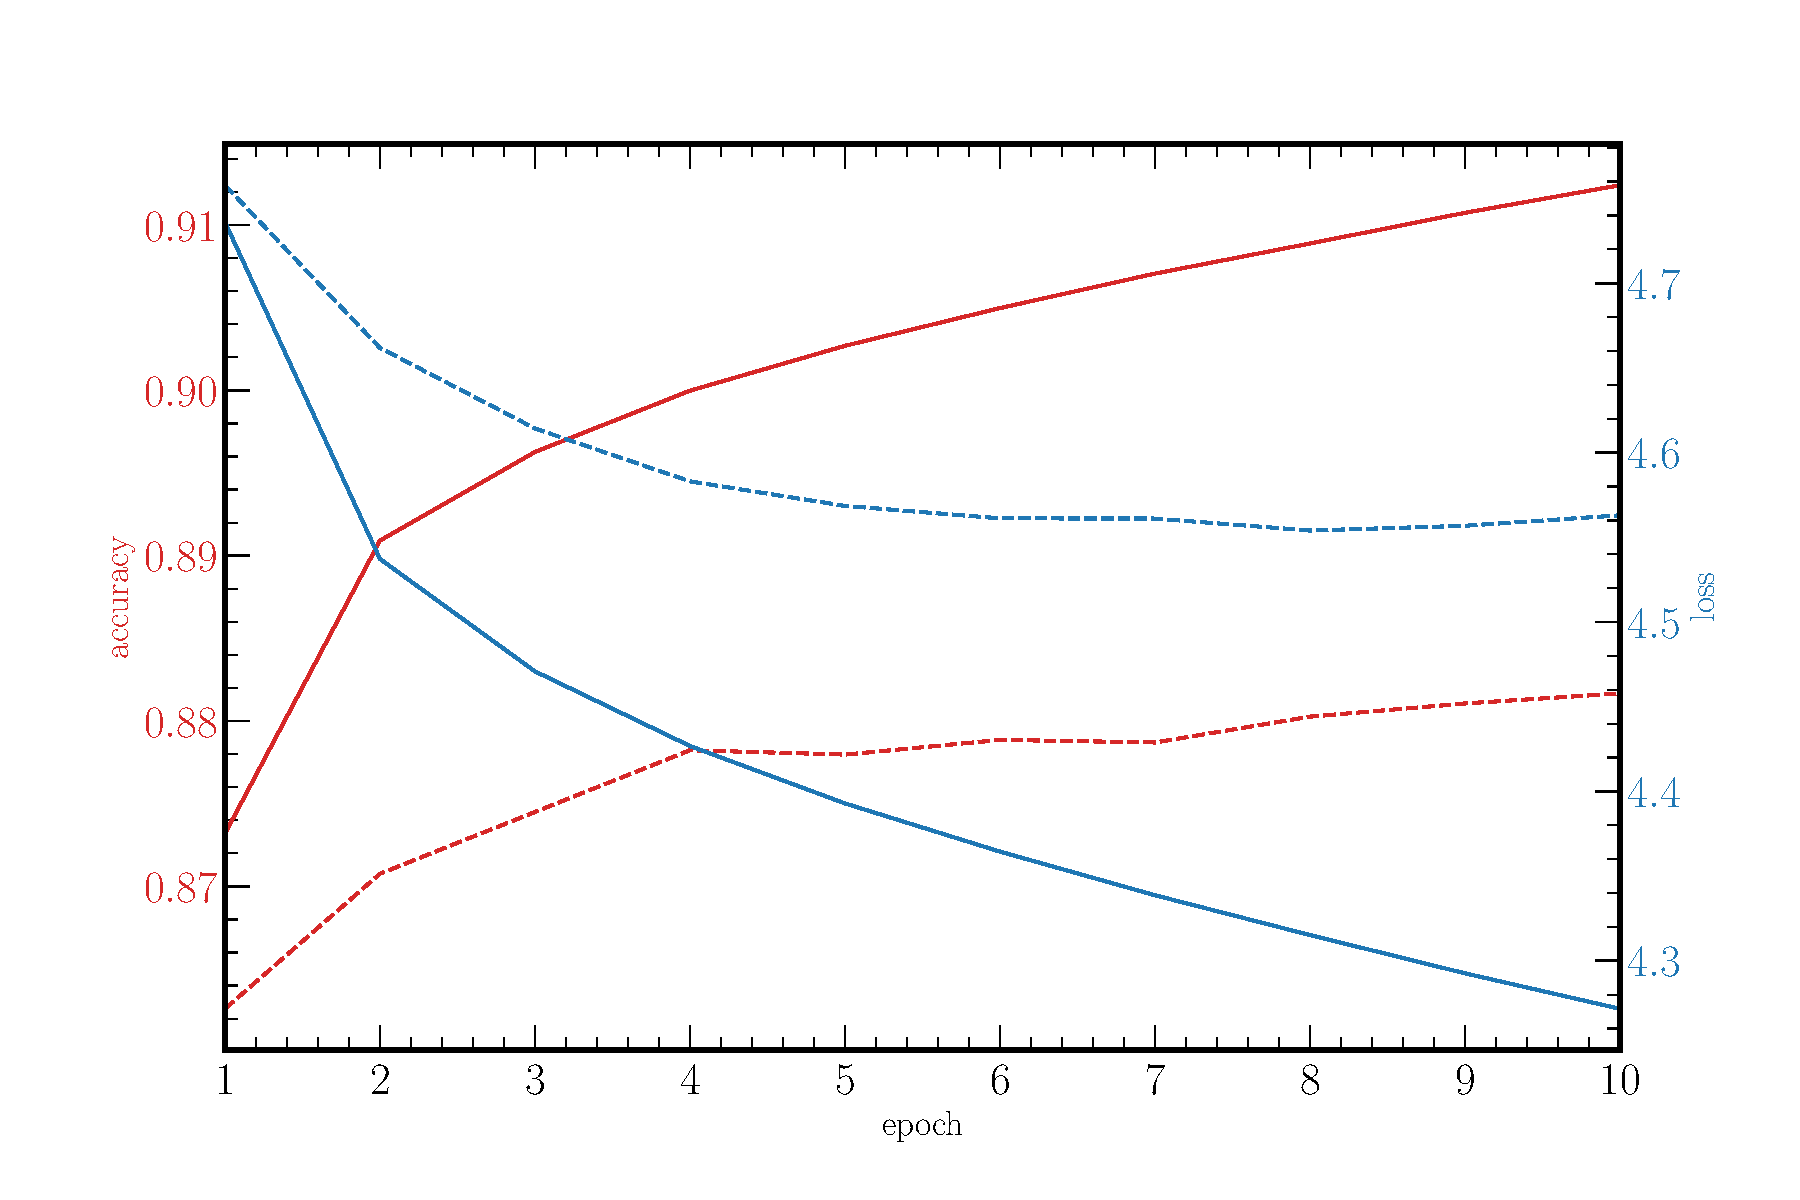
\includegraphics[width=0.7\textwidth]{diagrams/6-cvn/chipsnet/final_beam_history.pdf}
    \caption[Loss and accuracy throughout training for the beam classification network.]
    {Total loss and `combined category' accuracy for both the training dataset (solid) and
        validation dataset (dashed) throughout training for the beam classification network. The
        final network weights are taken at epoch 7 as shown by the vertical black line.}
    \label{fig:final_beam_history}
\end{figure}

\subsection{Energy estimation} %%%%%%%%%%%%%%%%%%%%%%%%%%%%%%%%%%%%%%%%%%%%%%%%%%%%%%%%%%%%%%%%%%%
\label{sec:cvn_specific_energy} %%%%%%%%%%%%%%%%%%%%%%%%%%%%%%%%%%%%%%%%%%%%%%%%%%%%%%%%%%%%%%%%%%

Accurate neutrino energy estimation is accomplished using multiple networks trained on separate
samples of $\nu_{e}$ and $\nu_{\mu}$ events across multiple CC interaction types. It is found that
separation such as this results in greater performance than if a single energy estimation network
or even separate $\nu_{e}$ and $\nu_{\mu}$ networks are trained. This is expected as a single set
of network weights is unlikely to be able to capture the specific topological features that
contribute to the energy for all types of event.

Alongside the primary neutrino energy regression task, additionally learning the primary charged
lepton energy and the interaction vertex position and time is found to improve performance.
Although this improvement is relatively small for neutrino energy estimation, it dramatically
improves primary charged lepton energy estimation when compared to being predicted alone. With two
energy tasks, the network is encouraged to learn how the primary charged lepton and neutrino
energies are related. As the interaction vertex position within the detector and hence distance
from the instrumented wall can impact the number of deposited photoelectrons, there is motivation
as to why these additional tasks are also helpful.

Separate networks are trained for each of CC-QE(CC-MEC), CC-Res, and CC-DIS for both $\nu_{e}$ and
$\nu_{\mu}$ events (8 in total) using 250000 corresponding simulated events each. Only events for
which the primary charged lepton is fully contained within the detector volume are considered. All
events (both $\nu_{\mu}$ and $\nu_{e}$) are generated using the expected \chips $\nu_{\mu}$ energy
spectrum to closely mimic the dominant $\nu_{\mu}$ beam component and appeared $\nu_{e}$ signal.
Each sample is split 95\% to 5\% for training and validation, respectively. Note that CC-QE and
CC-MEC neutrino energy estimation is combined as both have incredibly similar final state
topologies.

There are six outputs to each of the energy estimation networks:
\begin{enumerate}
    \item \textbf{Neutrino energy (1 neuron):} Returns the estimated neutrino energy. The
          mean-squared error loss function in Eq.~\ref{eq:mse} is used for training.
    \item \textbf{Charged lepton energy (1 neuron):} Returns the estimated primary charged lepton
          energy. The mean-squared error loss function in Eq.~\ref{eq:mse} is used for training.
    \item \textbf{Interaction vertex x-position (1 neuron):} Returns the estimated interaction
          vertex x-position. The mean-squared error loss function in Eq.~\ref{eq:mse} is used for
          training.
    \item \textbf{Interaction vertex y-position (1 neuron):} Returns the estimated interaction
          vertex y-position. The mean-squared error loss function in Eq.~\ref{eq:mse} is used for
          training.
    \item \textbf{Interaction vertex z-position (1 neuron):} Returns the estimated interaction
          vertex z-position. The mean-squared error loss function in Eq.~\ref{eq:mse} is used for
          training.
    \item \textbf{Interaction time (1 neuron):} Returns the estimated interaction time relative to
          the first PMT hit for each event. The mean-squared error loss function in
          Eq.~\ref{eq:mse} is used for training.
\end{enumerate}

Each network is allowed to train for up to 30 epochs using the SHERPA optimised hyperparameters:
$\eta_{0}=0.0002$, $c_{d}=0.5$, $p_{d}=0.1$, $\sigma_{r}=0.0$, and $n_{b}=128$, with a learnt
multi-task loss combination as given in Eq.~\ref{eq:multi_learnt}. Typically, only approximately
15 epochs are required to reach the minimum mean absolute error on the validation sample `neutrino
energy'. Early stopping typically halts training after approximately 20 epochs. An example of how
an energy estimation networks training typically proceeds is given in
Fig.~\ref{fig:final_energy_history}. Training each takes approximately 2 hours.

\begin{figure} % ENERGY HISTORY DIAGRAM %
    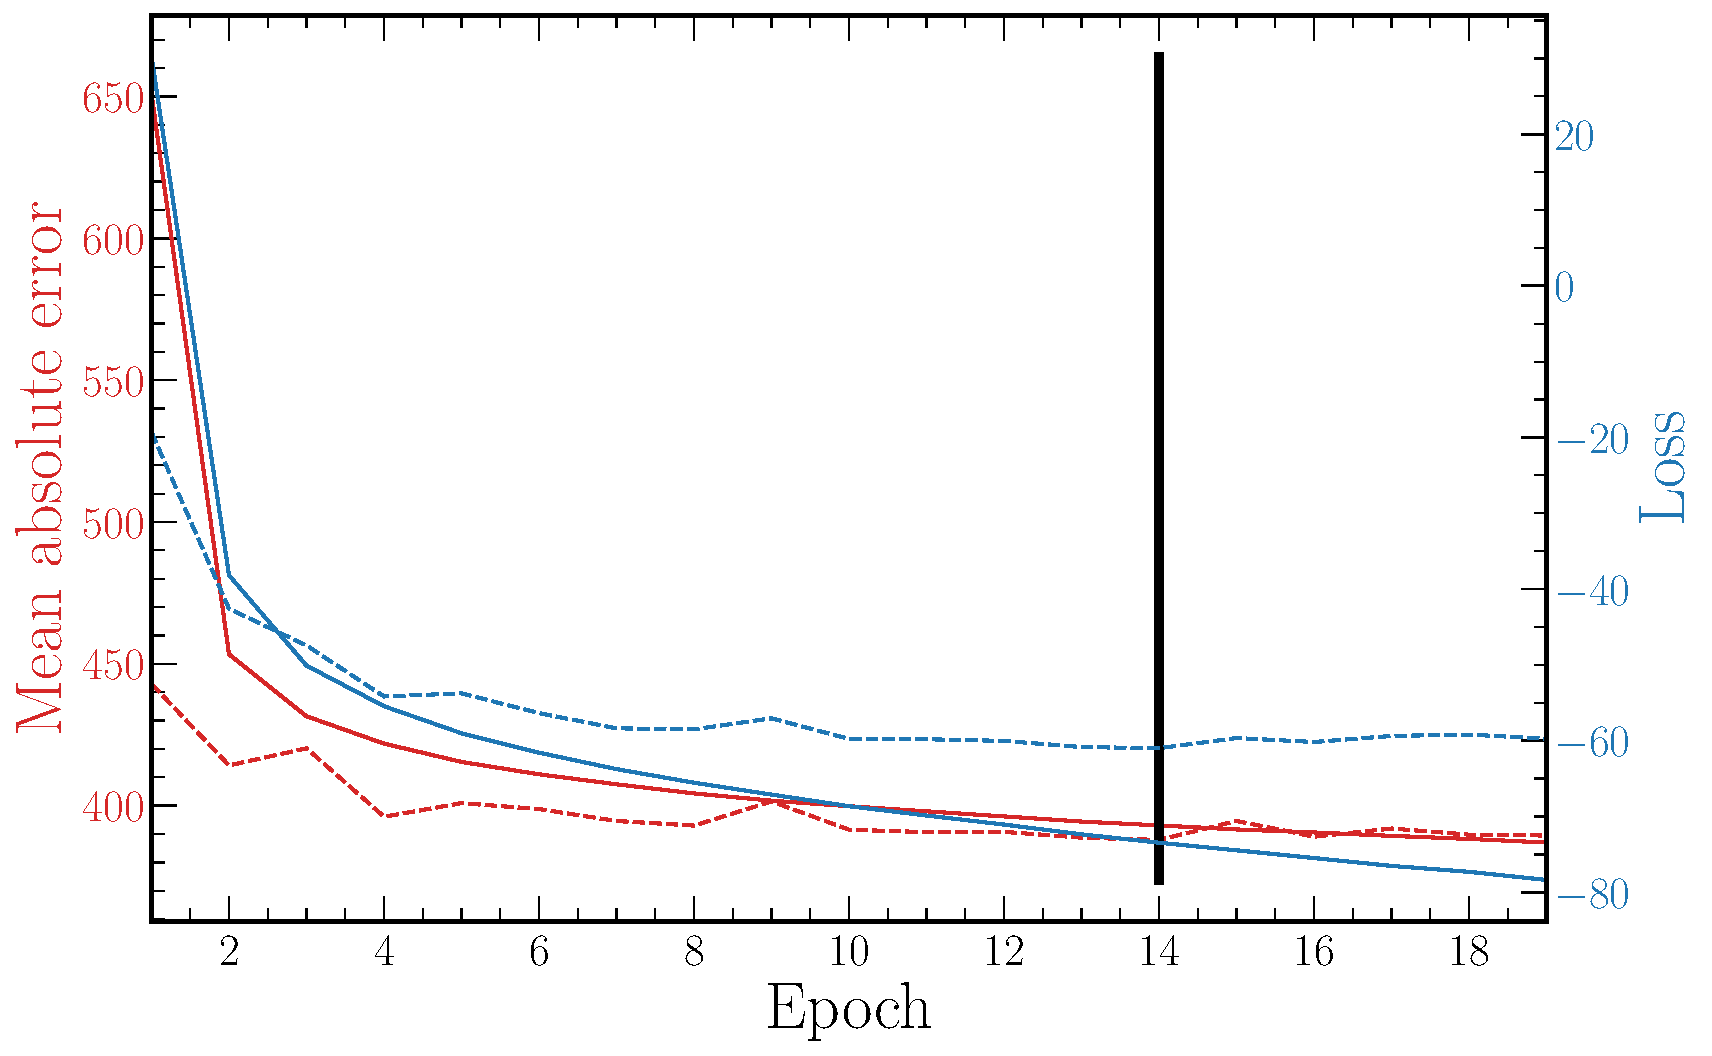
\includegraphics[width=0.7\textwidth]{diagrams/6-cvn/chipsnet/final_energy_history.pdf}
    \caption[Loss and mean absolute error throughout training for the beam classification network.]
    {Total loss and `neutrino energy' mean absolute error for both the training dataset (solid)
        and validation dataset (dashed) throughout training for the energy estimation network
        trained on CC-QE and CC-MEC $\nu_{e}$ events. The final network weights are taken at epoch
        14 as shown by the vertical black line.}
    \label{fig:final_energy_history}
\end{figure}

\section{Results} %%%%%%%%%%%%%%%%%%%%%%%%%%%%%%%%%%%%%%%%%%%%%%%%%%%%%%%%%%%%%%%%%%%%%%%%%%%%%%%%
\label{sec:cvn_results} %%%%%%%%%%%%%%%%%%%%%%%%%%%%%%%%%%%%%%%%%%%%%%%%%%%%%%%%%%%%%%%%%%%%%%%%%%

\subsection{Evaluation sample and preselection} %%%%%%%%%%%%%%%%%%%%%%%%%%%%%%%%%%%%%%%%%%%%%%%%%%%%%%%%%%%%%%%%%%%
\label{sec:cvn_results_sample} %%%%%%%%%%%%%%%%%%%%%%%%%%%%%%%%%%%%%%%%%%%%%%%%%%%%%%%%%%%%%%%%%%%

A statistically independent sample of events is used to evaluate the combined performance of the
trained CNNs. Generated in the same way as the training and validation samples, the evaluation
sample consists of 400000 beam and 350000 cosmic muon events. The beam events include the expected
$\nu_{\mu}$, $\bar{\nu}_{\mu}$, $\nu_{e}$ and $\bar{\nu}_{e}$ components of the beam as well as
events generated to mimic the appeared $\nu_{e}$ component. In this work, only the neutrino mode
(forward horn current) of NuMI beam operation is considered for simplicity.

All evaluation events are weighted to match the expected spectrum in the 5 kton \chipsfive
detector, generated using the expected unoscillated flux, cross-sections, and standard oscillation
probabilities. Additional weighting also scales the events to match running in the NuMI beam for a
year, corresponding to $6\times 10^{20}$ protons on target (POT). For cosmic events, a rate of
\unit{5.1}{\mathrm{kHz}} with \unit{50}{\mathrm{m}} of overburden is assumed, rejecting events
that fall outside the NuMI beam spill window. For simplicity, the neutrino and antineutrino
components of the beam are also combined as they are impossible to tell apart in practice. The
final weighted spectrum of events is shown in Fig.~\ref{fig:explore_osc_fluxes}. Furthermore, the
evaluation sample contains the expected combination of underlying neutrino interaction types, as
shown in Fig.~\ref{fig:explore_stacked_int_types}.

\begin{figure} % OSC FLUXES DIAGRAM %
    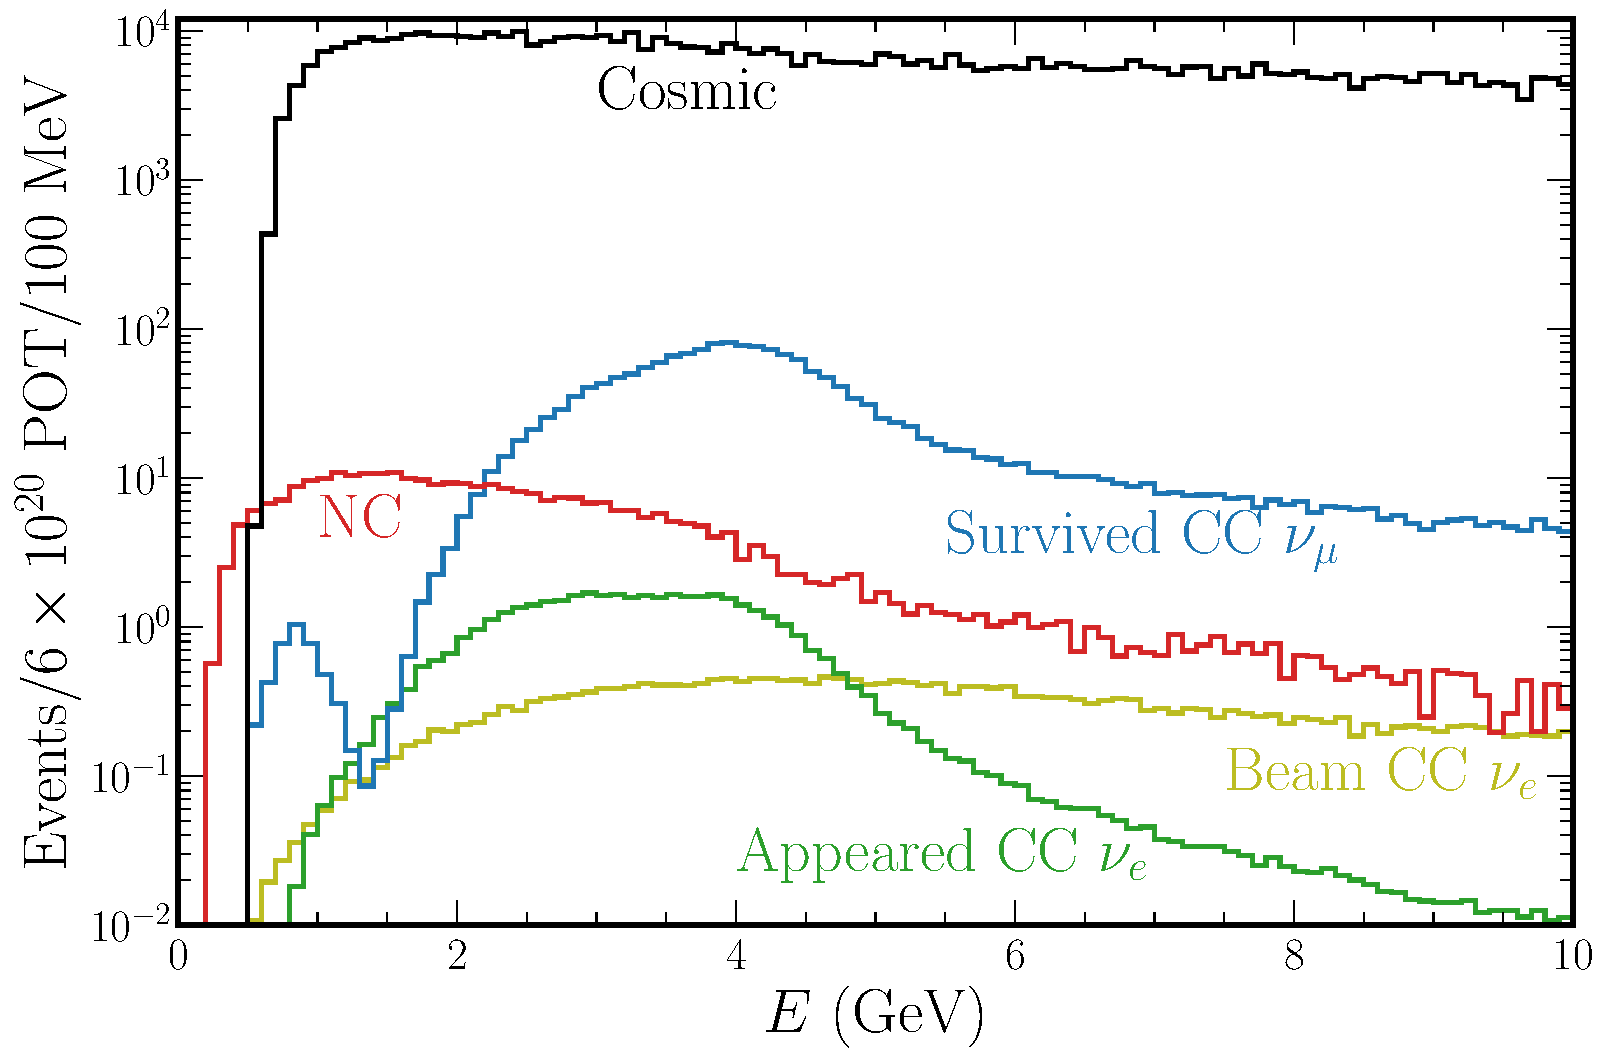
\includegraphics[width=0.7\textwidth]{diagrams/6-cvn/chipsnet/explore_osc_fluxes.pdf}
    \caption[Weighted spectrum of evaluation sample events.]
    {The weighted spectrum of events contained within the evaluation sample. The weighting is
        designed to mimic the expected event spectrum of the \chipsfive detector. Beam events are
        weighted by combining the expected un-oscillated flux with cross-sections and standard
        oscillation probabilities, while cosmic events are weighted using the expected rate and
        overburden. Shown in blue, green and olive are the survived CC $\nu_{\mu}$, appeared CC
        $\nu_{e}$ and the intrinsic beam CC $\nu_{e}$ spectra respectively, binned in terms of
        their neutrino energy. Additionally, shown in red is the NC event spectra binned in terms
        of the energy of the hadronic system (excluding the outgoing neutrino energy) to represent
        more accurately the energy visible to the detector. Finally, shown in black is the cosmic
        muon event spectra binned in terms of the muon energy.}
    \label{fig:explore_osc_fluxes}
\end{figure}

\begin{figure} % STACK INT TYPES DIAGRAM %
    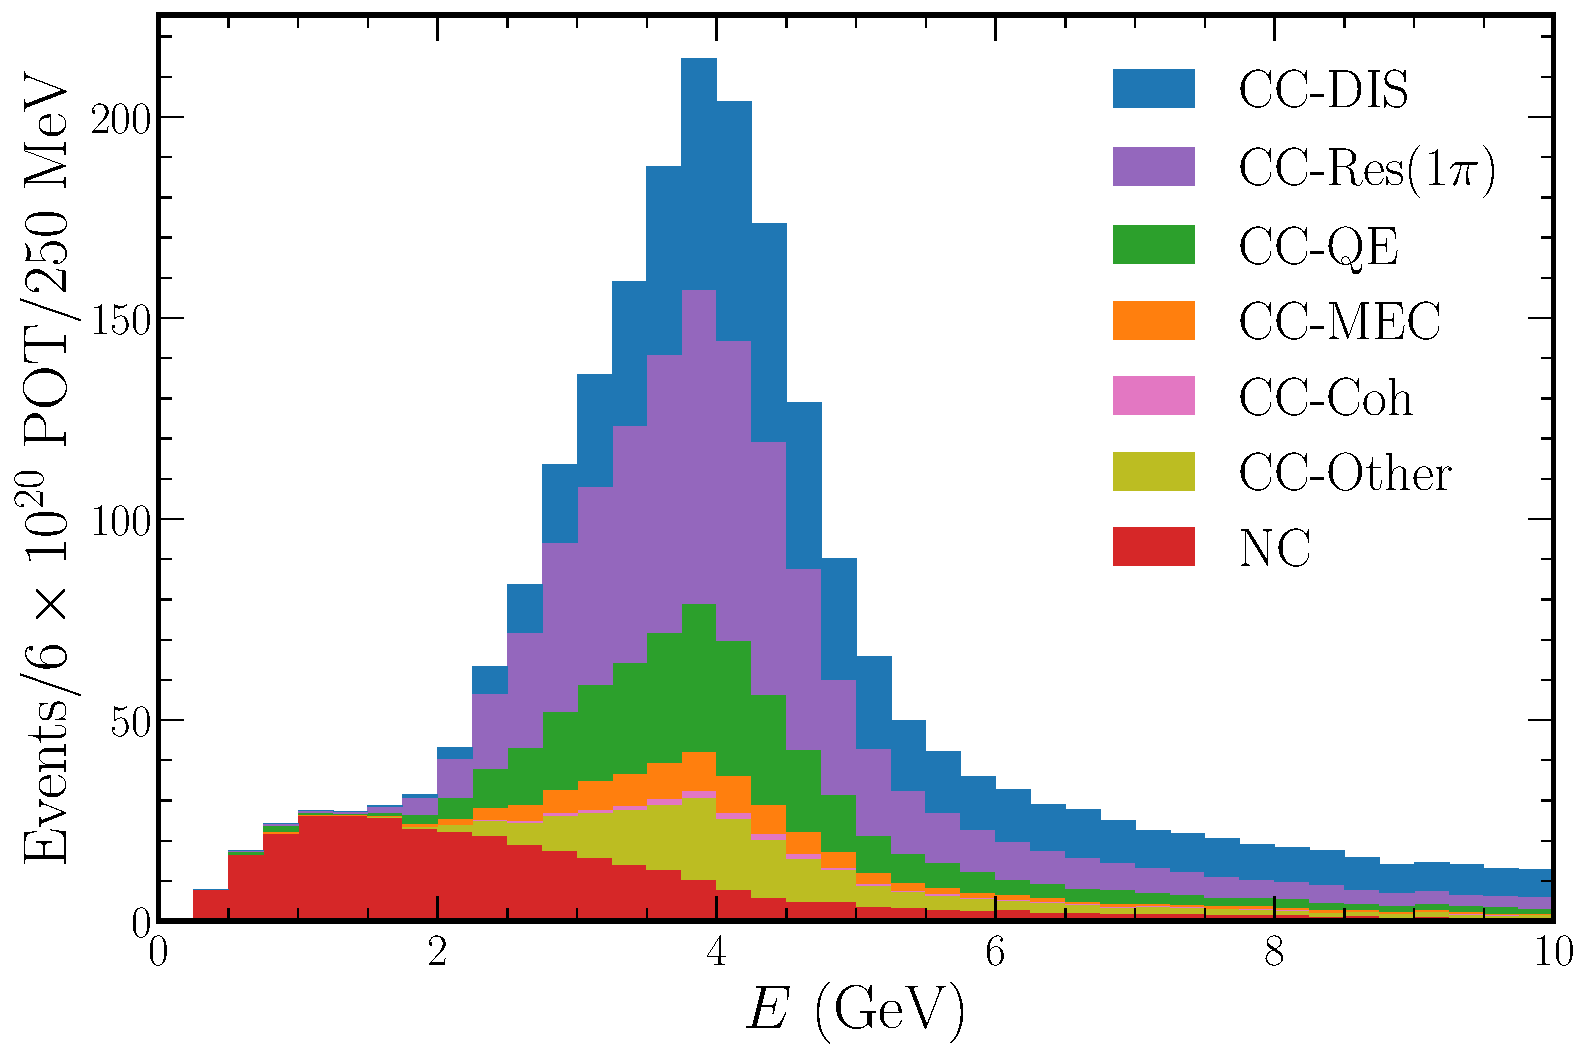
\includegraphics[width=0.7\textwidth]{diagrams/6-cvn/chipsnet/explore_stacked_int_types.pdf}
    \caption[Weighted spectrum of interaction types within the evaluation sample.]
    {The weighted spectrum of beam events contained within the evaluation sample separated by
        interaction type. Both $\nu_{\mu}$ and $\nu_{e}$ events are included. CC events are binned
        in terms of neutrino energy while NC events are binned in terms of the energy of the
        hadronic system.}
    \label{fig:explore_stacked_int_types}
\end{figure}

Separate from the CNN driven work, a simple preselection is applied to all events in the
evaluation sample. Designed to reject cosmic muon and NC events while keeping the efficiency of CC
beam events high, the preselection consists of four simple cuts, shown in
Fig.~\ref{fig:explore_simple_cuts}. Firstly, the total collected charge (photoelectrons) across
all PMTs in the event must be greater than 250 photoelectrons. Secondly, the maximum Hough
transform space height must be greater than 250 photoelectrons. Thirdly, the leading seed
$\cos(\theta)$ direction must be between $\pm$0.7. Finally, the leading seed $\phi$ direction must
be between $\pm$1.1 radians. The first two cuts reject low energy events which are usually NC in
nature, while the last two reject events whose activity is not along the beamline, typically
cosmic events.

\begin{figure} % SIMPLE CUTS DIAGRAM %
    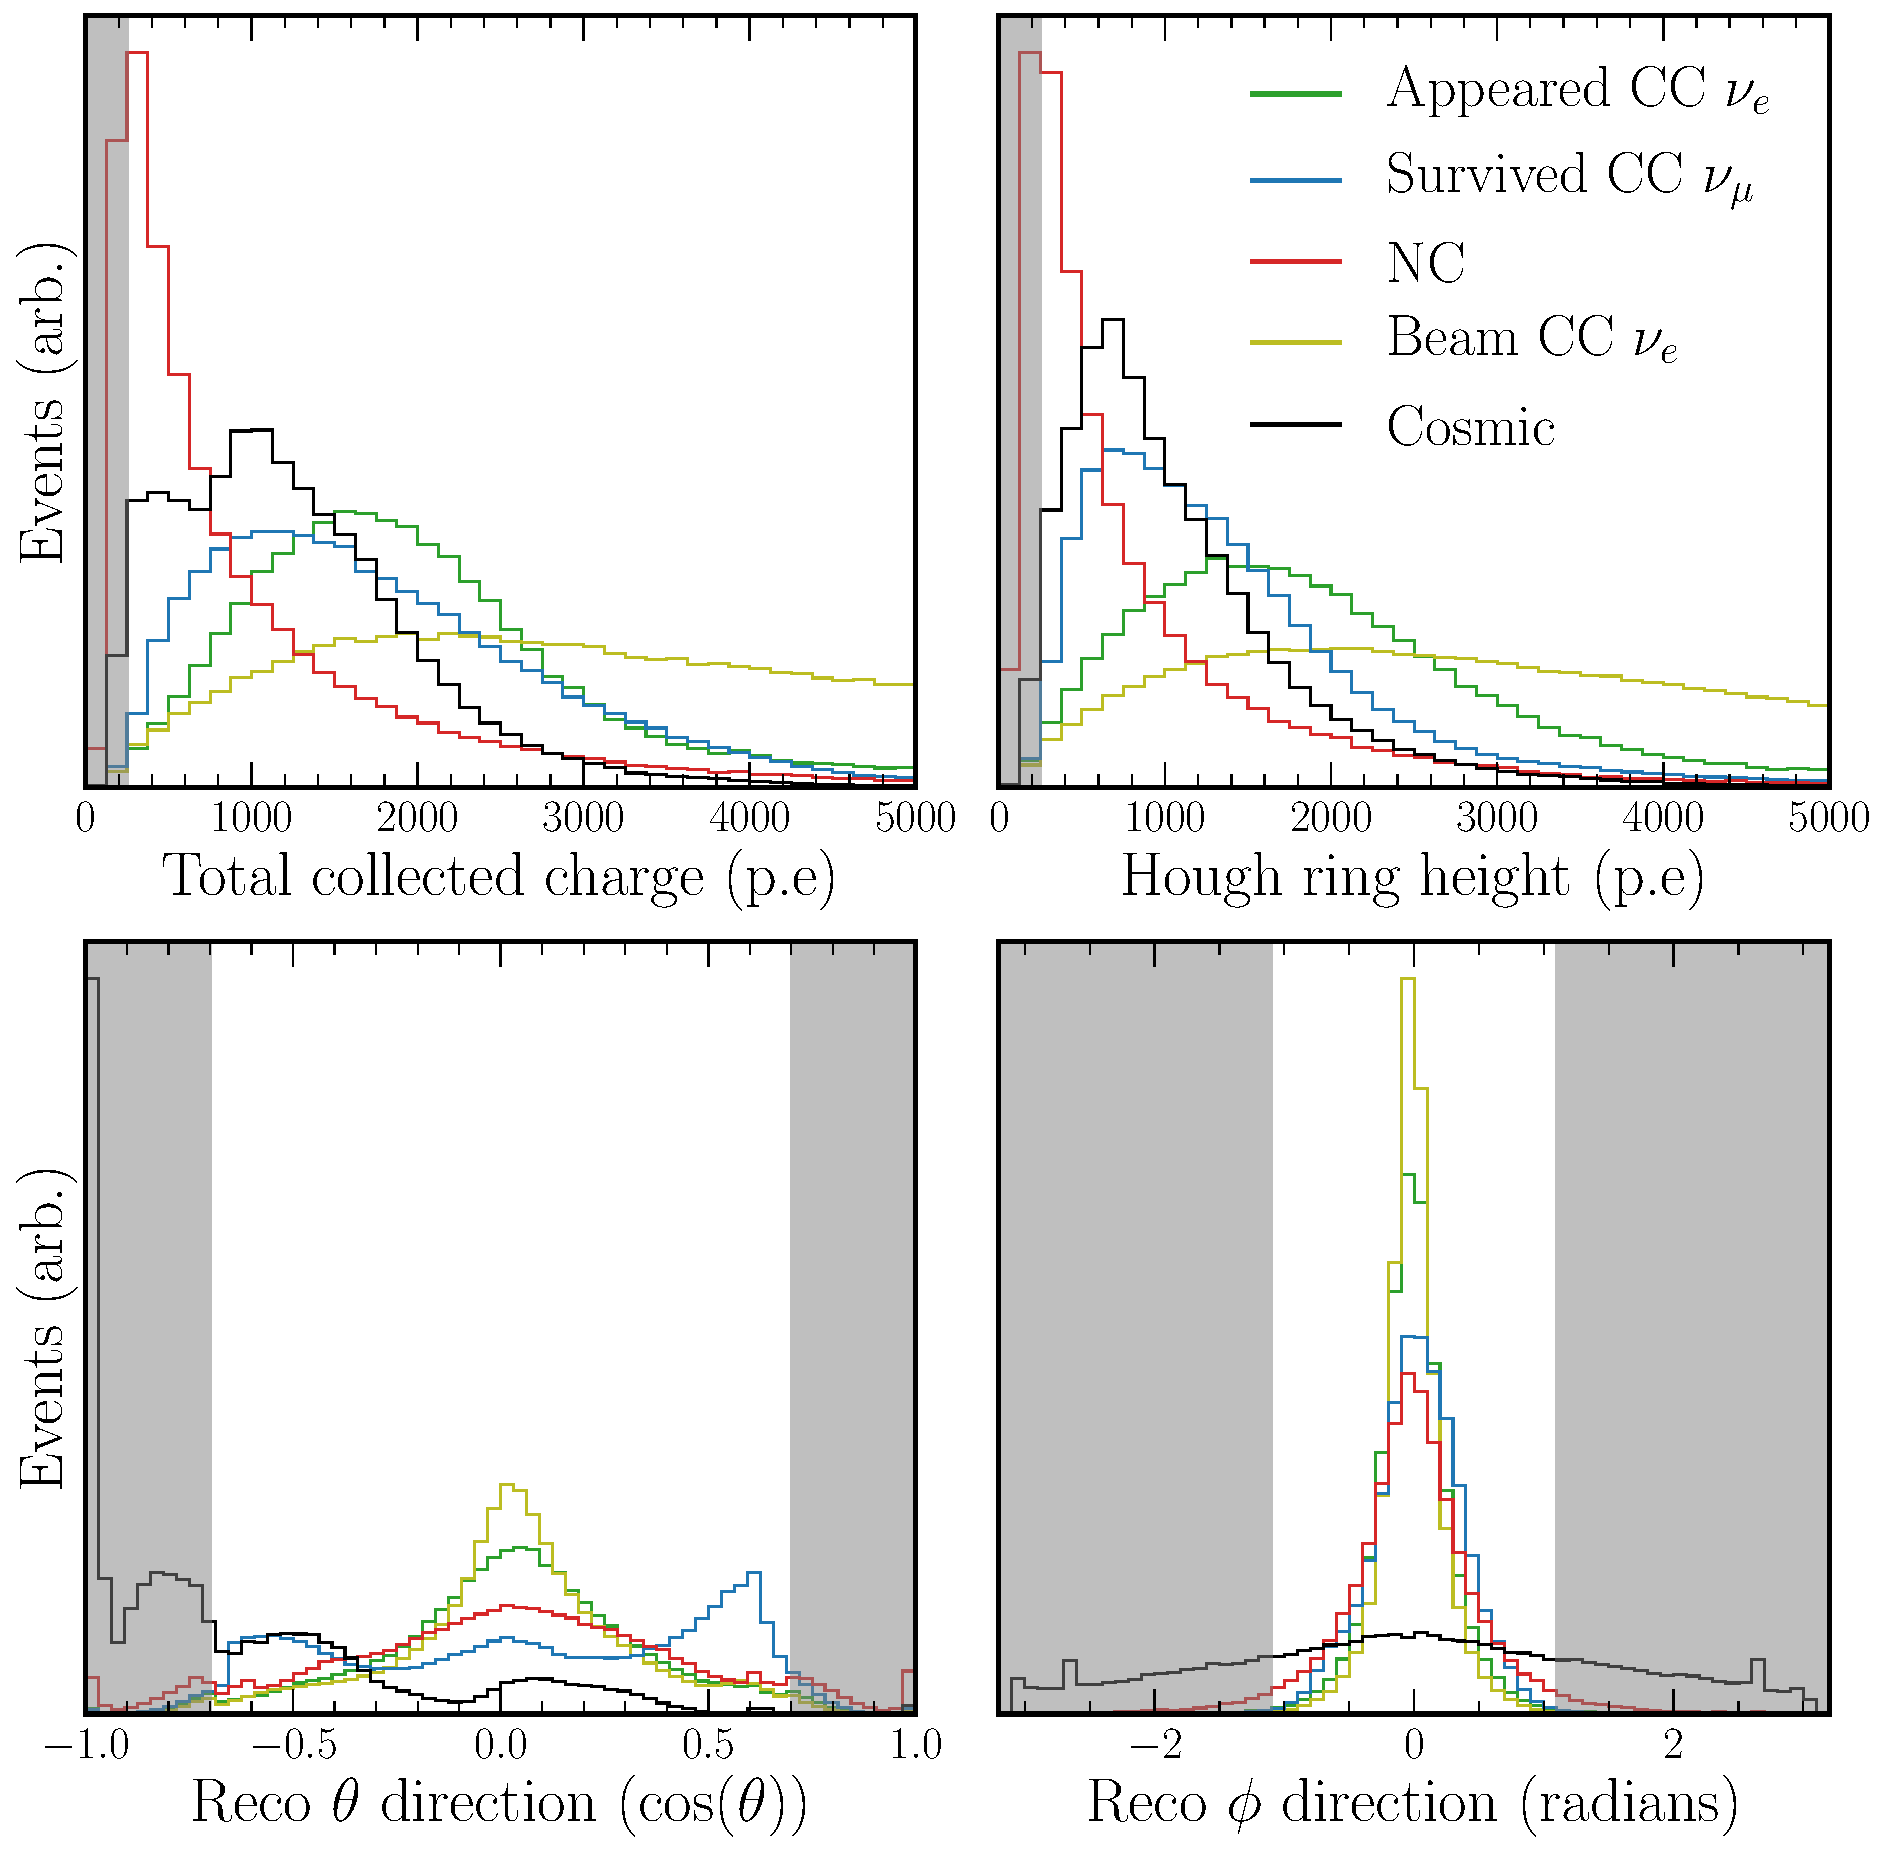
\includegraphics[width=0.8\textwidth]{diagrams/6-cvn/chipsnet/explore_simple_cuts.pdf}
    \caption[Plot detailing preselection cuts.]
    {Plots detailing how the four simple cuts that make up the preselection affect the different
        event categories. The greyed out areas show the regions for which events are rejected.}
    \label{fig:explore_simple_cuts}
\end{figure}
\subsection{Cosmic rejection and containment} %%%%%%%%%%%%%%%%%%%%%%%%%%%%%%%%%%%%%%%%%%%%%%%%%%%%
\label{sec:cvn_results_cosmic} %%%%%%%%%%%%%%%%%%%%%%%%%%%%%%%%%%%%%%%%%%%%%%%%%%%%%%%%%%%%%%%%%%%

The `cosmic score' output from the trained cosmic rejection network gives excellent separation
between beam like (output close to zero) and cosmic like (output close to one) events, as can be
seen in Fig.~\ref{fig:cosmic_outputs}. Importantly, the vast majority of beam events are
associated with a score incredibly close to zero as is more clearly shown in
Fig.~\ref{fig:cosmic_zoomed_outputs}. Given this, a tight cut of a `cosmic score' below 0.0001 is
chosen by inspection to accept beam like events. Out of the total 350000 cosmic events in the
evaluation sample, all are rejected by this cut along with preselection. Without the addition of
the second `escapes score' output, a trained cosmic rejection network instead allow five cosmic
events to pass preselection and the cut above.

\begin{figure} % COSMIC OUTPUTS DIAGRAM %
    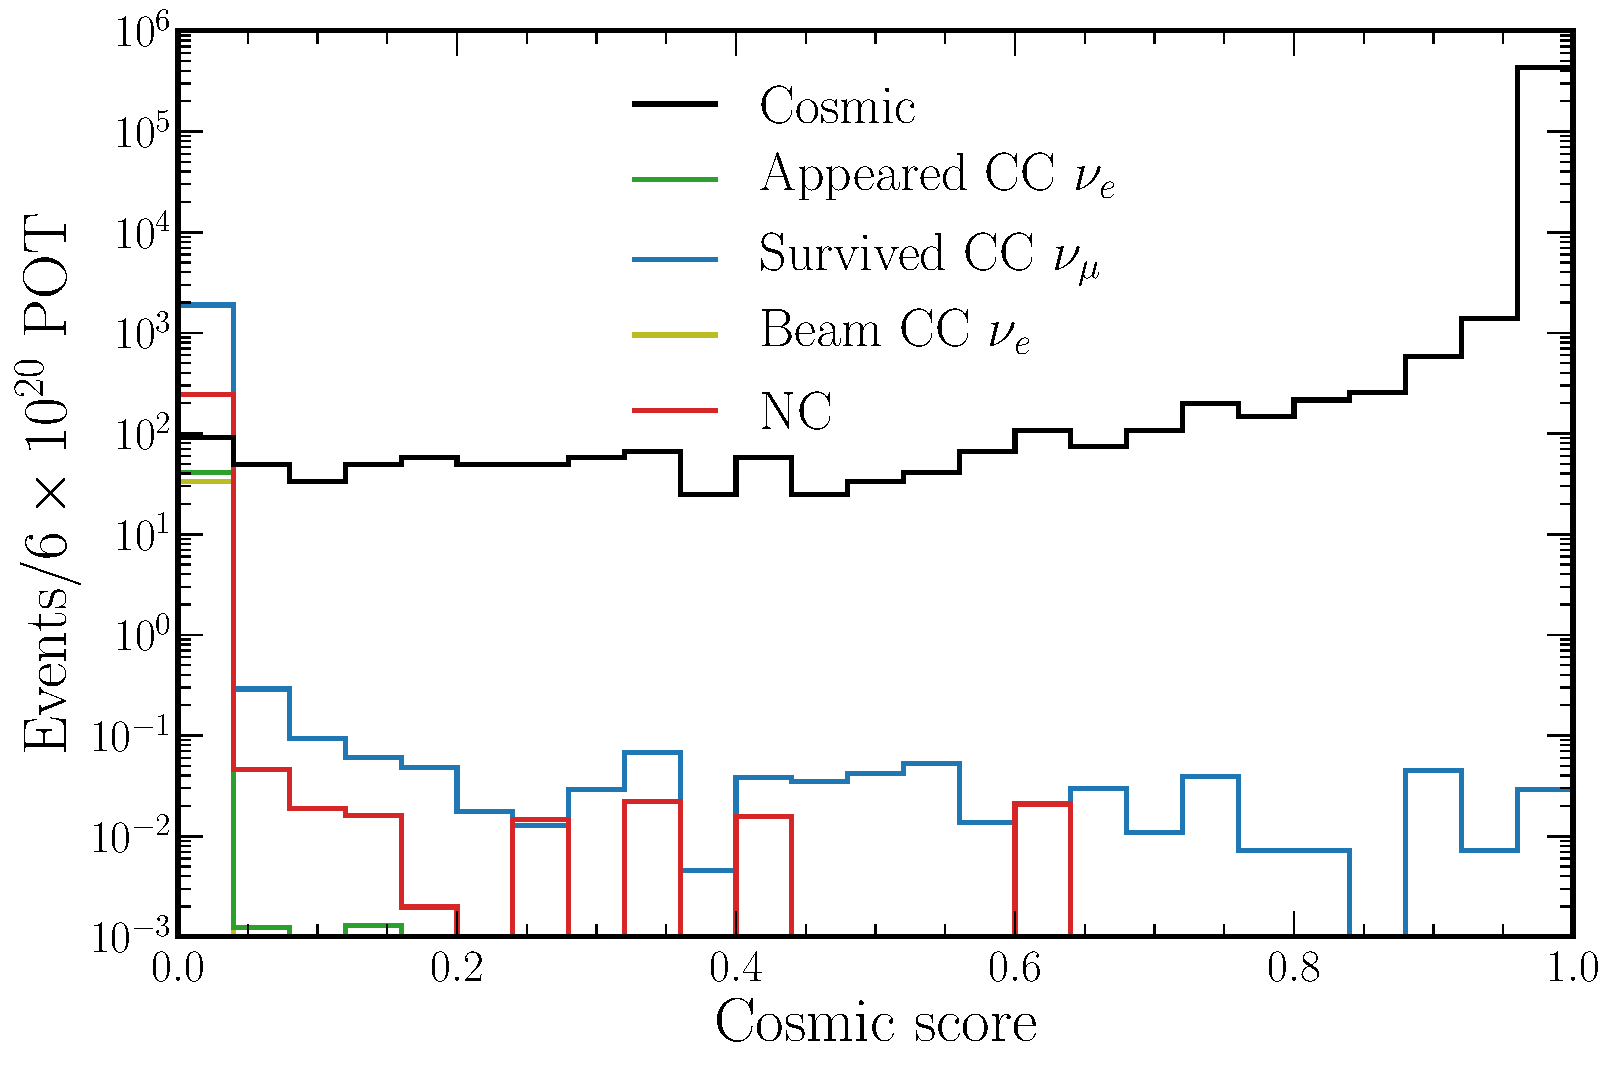
\includegraphics[width=0.7\textwidth]{diagrams/6-cvn/chipsnet/final_cosmic_outputs.pdf}
    \caption[Distribution of cosmic score output values.]
    {Distribution of `cosmic score' output values for the different event categories. A score
        close to one signifies a cosmic like event, while a score close to zero corresponds to a
        beam like event.}
    \label{fig:cosmic_outputs}
\end{figure}

\begin{figure} % COSMIC OUTPUTS ZOOMED DIAGRAM %
    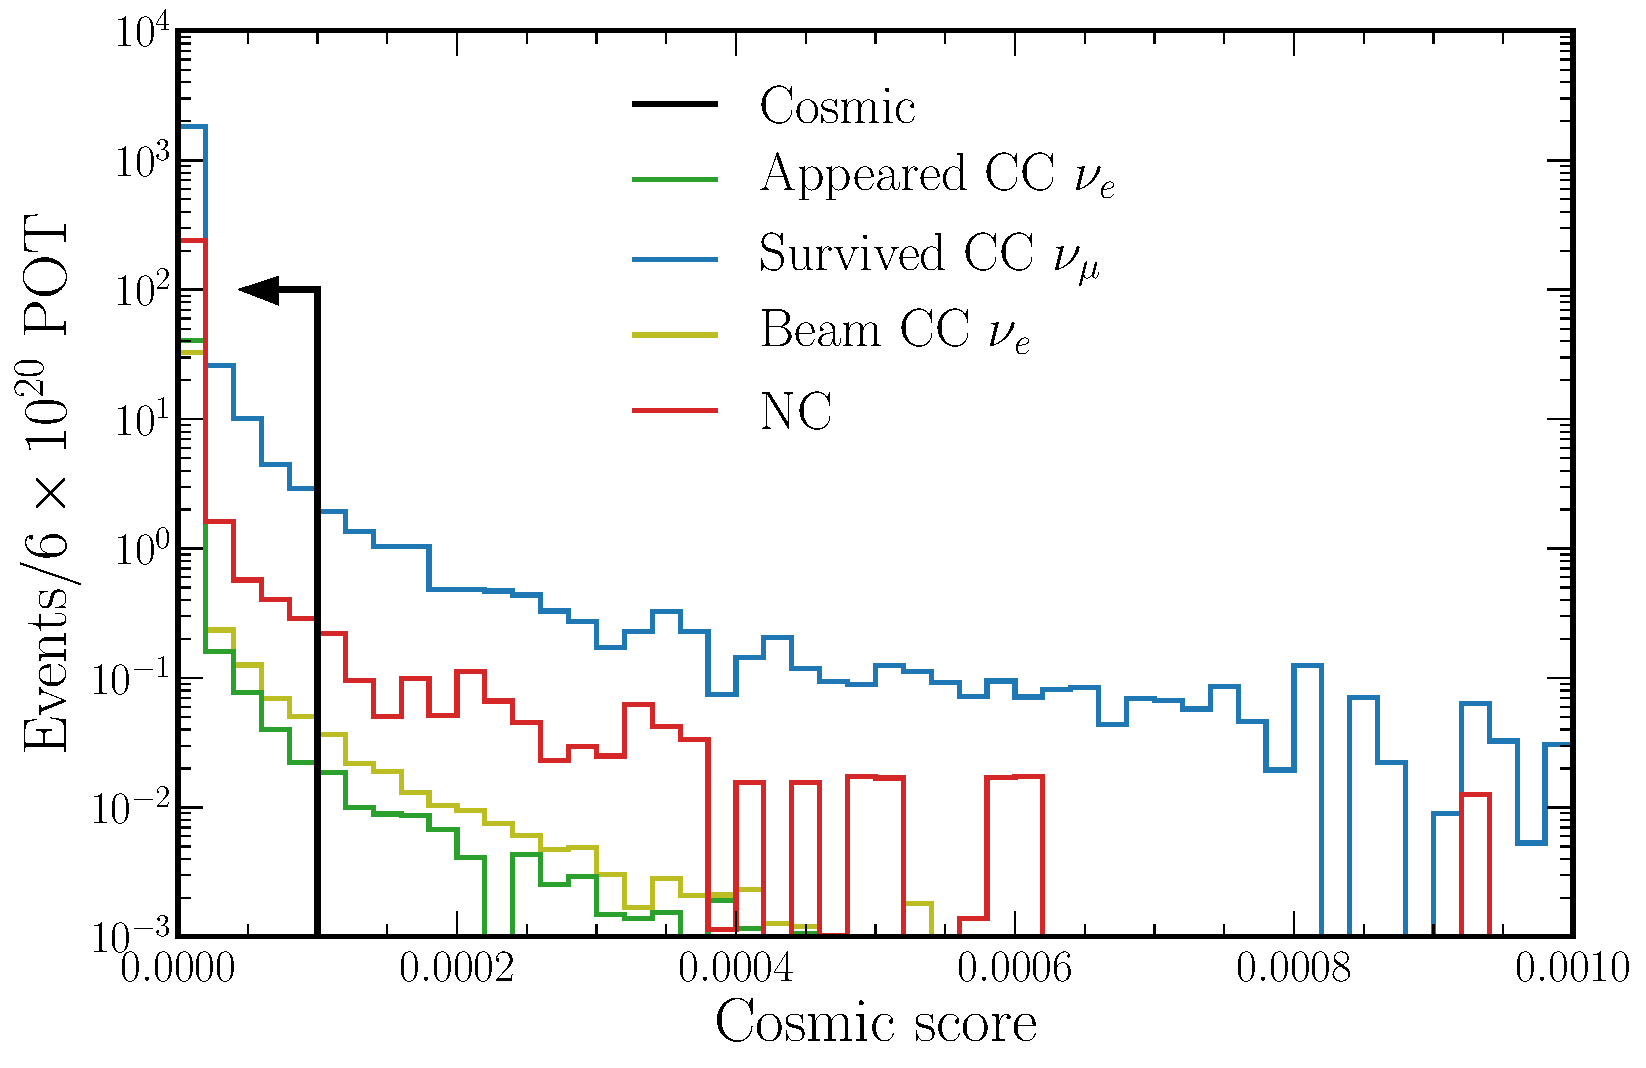
\includegraphics[width=0.7\textwidth]{diagrams/6-cvn/chipsnet/final_cosmic_zoomed_outputs.pdf}
    \caption[Distribution of cosmic score output values close to zero.]
    {Distribution of `cosmic score' output values close to zero for the different event
        categories. The cosmic rejection cut value at 0.0001 is shown with the arrow showing the
        events that are selected. Note that no cosmic events are within the range shown due to the
        statistical limitations of the evaluation sample.}
    \label{fig:cosmic_zoomed_outputs}
\end{figure}

It is crucial for accurate neutrino energy estimation that the activity of an event is fully
contained within the volume of the detector. If charged event particles instead leave the detector
and emit Cherenkov radiation not captured by PMTs, it can be incredibly difficult to estimate the
resulting missing energy and hence the neutrino energy. Within the \chipsfive detector, this is
particularly important for CC $\nu_{\mu}$ events for which only 44\% of the long track primary
charged muons are fully contained within the detector volume.

Therefore, the second output from the cosmic rejection network `escapes score' is also used to
select events. Although this only considers the primary charged lepton instead of all event
particles, it still acts as a reasonable simplified proxy for event containment. The distribution
of `escapes score' output values from the trained cosmic rejection network is shown in
Fig.~\ref{fig:final_escapes_outputs}.

A value below 0.5 is chosen by inspection to select events for which the primary charged lepton is
fully contained within the detector. With this selection, 97\%(96\%) of CC $\nu_{\mu}$ events for
which the primary charged lepton is contained within(escapes) the detector are classified
correctly, resulting in a 95\% purity for the selected `contained' CC $\nu_{\mu}$ sample. As
expected, the vast majority of CC $\nu_{e}$ and NC events are selected.

\begin{figure} % ESCAPES OUTPUTS DIAGRAM %
    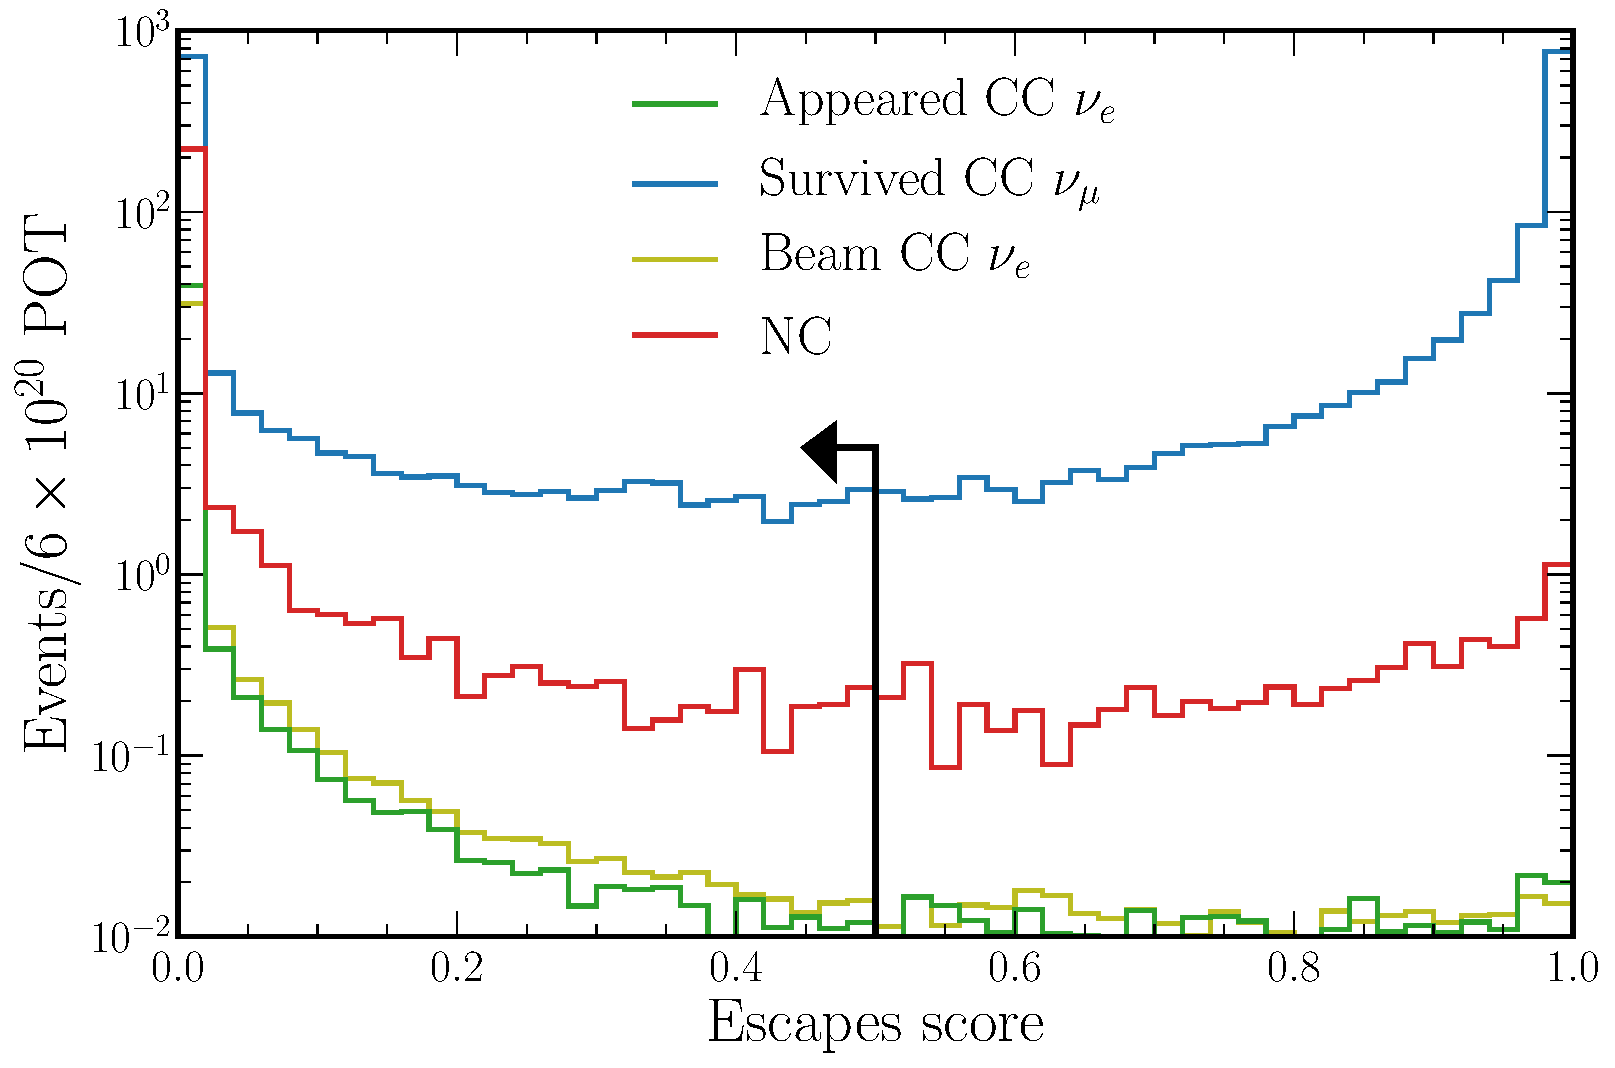
\includegraphics[width=0.7\textwidth]{diagrams/6-cvn/chipsnet/final_escapes_outputs.pdf}
    \caption[Distribution of escapes score output values.]
    {Distribution of `escapes score' output values for the different event categories. A score
        close to one signifies an escaped primary charged lepton like event, while a score close
        to zero corresponds to a contained primary charged lepton like event. The containment cut
        value at 0.5 is shown with the arrow representing the events that are selected.}
    \label{fig:final_escapes_outputs}
\end{figure}

The total number of events per year that pass each successive cut (including preselection) for
each event category is shown in Table.~\ref{tab:selection}. Both CC $\nu_{e}$ categories are
selected with an efficiency greater than 90\%, while CC $\nu_{\mu}$ events are intentionally
reduced to 40\% efficiency to ensure they are fully contained. Furthermore, NC events are found to
be primarily rejected by the preselection, while cosmic events are heavily rejected by both the
preselection and `cosmic score' cuts.

\begin{table}
    \begin{tabular}{lccccc}
                           & Appeared CC $\nu_{e}$ & Survived CC $\nu_{\mu}$ & Beam CC $\nu_{e}$ & NC    & Cosmic  \\
        \midrule
        Total events       & 44.2                  & 2045.9                  & 35.1              & 348.7 & 1211000 \\
        After preselection & 41.2                  & 1889.5                  & 33.5              & 239.6 & 249260  \\
        After cosmic cut   & 41.1                  & 1874.4                  & 33.4              & 238.0 & 0.0     \\
        After escapes cut  & 40.8                  & 818.0                   & 33.0              & 231.0 & 0.0     \\
        \midrule
        Efficiency         & 0.923                 & 0.400                   & 0.940             & 0.662 & 0.000   \\
    \end{tabular}
    \caption[Number of events passing basic cuts for each event category.]
    {Table showing the total number of events and the number that pass successive contained beam
        selection cuts for the different event categories. Those that pass the preselection, the
        `cosmic score' cut, and the `escapes score' cut are shown.}
    \label{tab:selection}
\end{table}

When compared to the approximately 1.2 million expected cosmic events per year, the zero out of
350000 evaluation events that are selected are not statistically significant. However, due to
computational constraints, the generation of a sufficiently sized cosmic evaluation sample is
deemed infeasible for this work.

To more accurately gauge the number of cosmic events likely to be classified as beam events, we
consider the more statistically significant number that passes a loose `cosmic score' cut below a
value of 0.9. In this case, 501 out of 350000 evaluation sample cosmic events are selected, which
when weighted corresponds to 2384 events per year. After the preselection and `escapes score' cuts
have also been applied only 38 or when weighted 180 cosmic events survive, corresponding to a
rejection factor of $1.5\times10^{-4}$.

Furthermore of the surviving 180 cosmic events, 95 are selected as CC $\nu_{\mu}$ events and zero
as CC $\nu_{e}$ events by the beam classification network, detailed in the following section. This
incredibly generous estimation, therefore, predicts a 10\% contamination for the beam CC
$\nu_{\mu}$ selection and a negligible contamination for the beam CC $\nu_{e}$ selection. In
reality, both are likely to be lower. This is comparable to the approximately $5\%$ cosmic
contamination of the CC $\nu_{\mu}$ sample seen by NoVA. Due to the constraints of the evaluation
sample outlined above, we do not consider cosmic events for the rest of the results section.

\subsection{Beam classification} %%%%%%%%%%%%%%%%%%%%%%%%%%%%%%%%%%%%%%%%%%%%%%%%%%%%%%%%%%%%%%%%%
\label{sec:cvn_results_beam} %%%%%%%%%%%%%%%%%%%%%%%%%%%%%%%%%%%%%%%%%%%%%%%%%%%%%%%%%%%%%%%%%%%%%

The output values from each of the `combined category' neurons of the trained beam classification
network give the probability score that an event belongs to the corresponding category. As the
output neuron scores collectively sum to one, the highest-scoring neuron can be used to classify
events as either CC $\nu_{e}$, CC $\nu_{\mu}$, or NC in nature.
Fig.~\ref{fig:final_comb_cat_confusion}, shows the resulting classification matrix for this
approach.

\begin{figure} % FINAL COMB CAT CONFUSION DIAGRAM %
    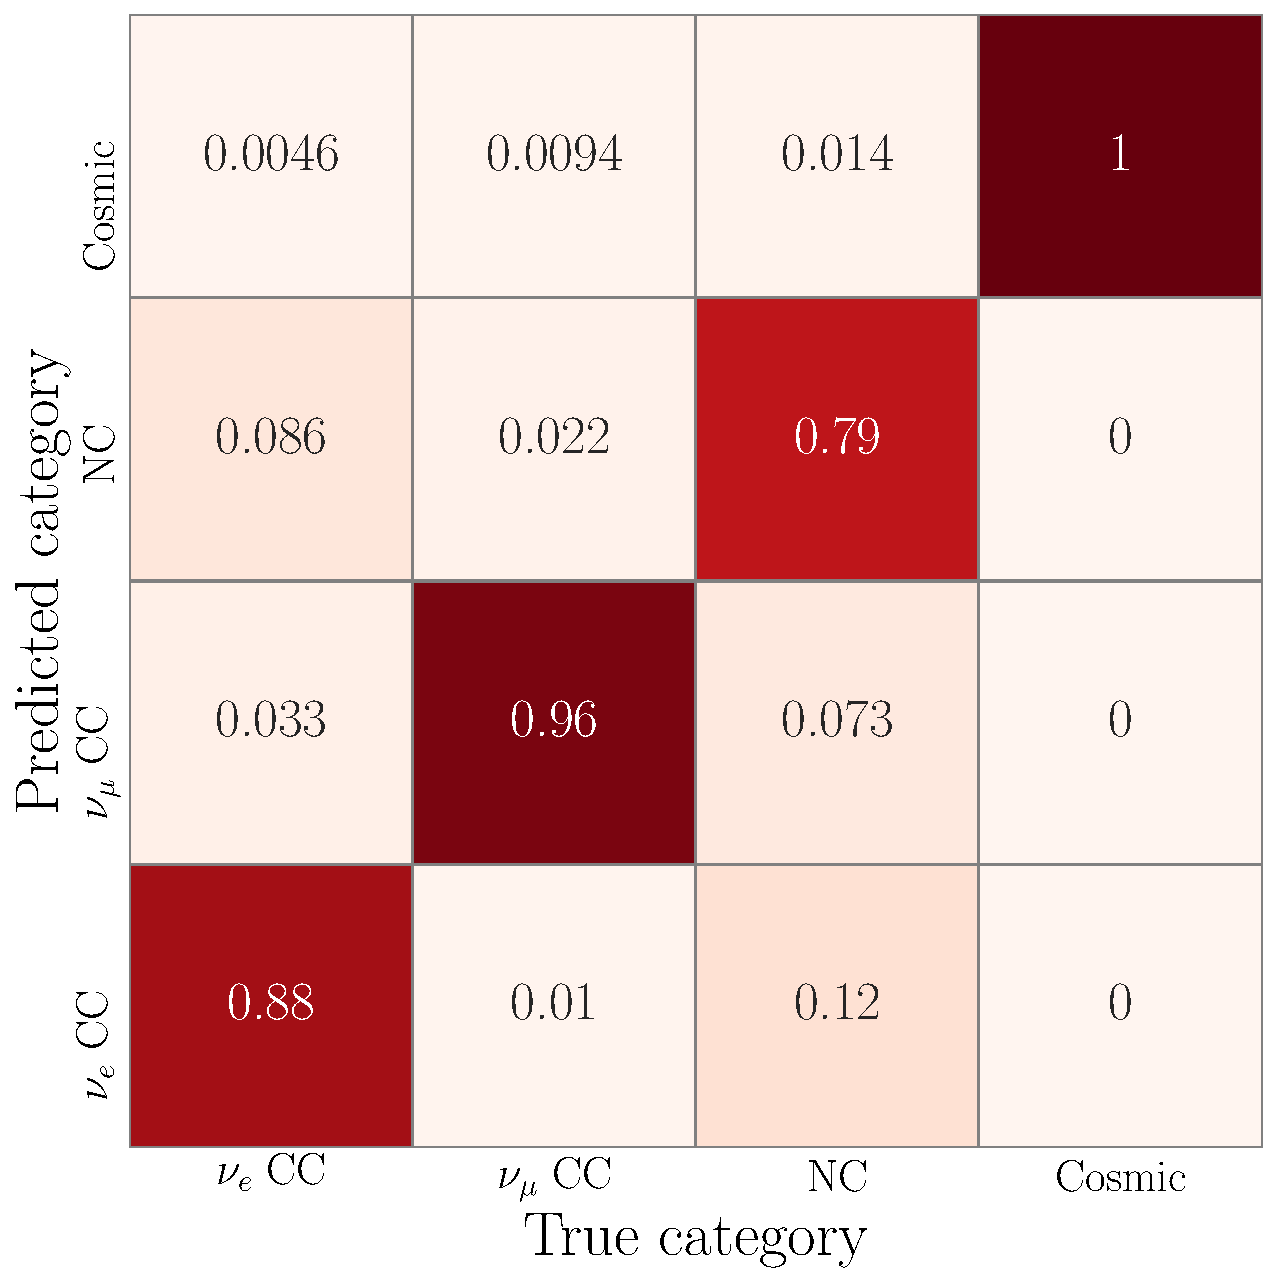
\includegraphics[width=0.6\textwidth]{diagrams/6-cvn/chipsnet/final_comb_cat_confusion.pdf}
    \caption[Classification matrix for the `combined category' output of the beam classification
        network.]
    {Classification matrix for the `combined category' output of the trained beam classification
        network. Events are simply classified using the categorical score for which they have the
        highest value. The numbers shown are the fraction of true category events that are
        classified into each of the three possible categories.}
    \label{fig:final_comb_cat_confusion}
\end{figure}

To access the beam classification performance more rigorously it is instead common to calculate a
selection score for each of the output categories, found by maximising a figure-of-merit. All
events above the optimised score are then accepted as signal. In this work the figure-of-merit
$\mathrm{efficiency}\times\mathrm{purity}$ is optimised to give an efficient sample. Below are the
results for both appeared CC $\nu_{e}$ and survived CC $\nu_{\mu}$ selections.

\subsubsection*{CC $\nu_{e}$ selection} %%%%%%%%%%%%%%%%%%%%%%%%%%%%%%%%%%%%%%%%%%%%%%%%%%%%%%%%%%

The distribution of CC $\nu_{e}$ scores for the different event categories is shown in
Fig.~\ref{fig:final_beam_nuel_outputs}. Very strong separation between appeared CC $\nu_{e}$
signal and both CC $\nu_{\mu}$ and NC background events is achieved, especially given the large
discrepancy in sample size. As no attempt is made to separate the appeared CC $\nu_{e}$ signal
component from the intrinsic beam CC $\nu_{e}$ background, both are clustered with scores close to
one as expected.

\begin{figure} % BEAM OUTPUTS NUEL DIAGRAM %
    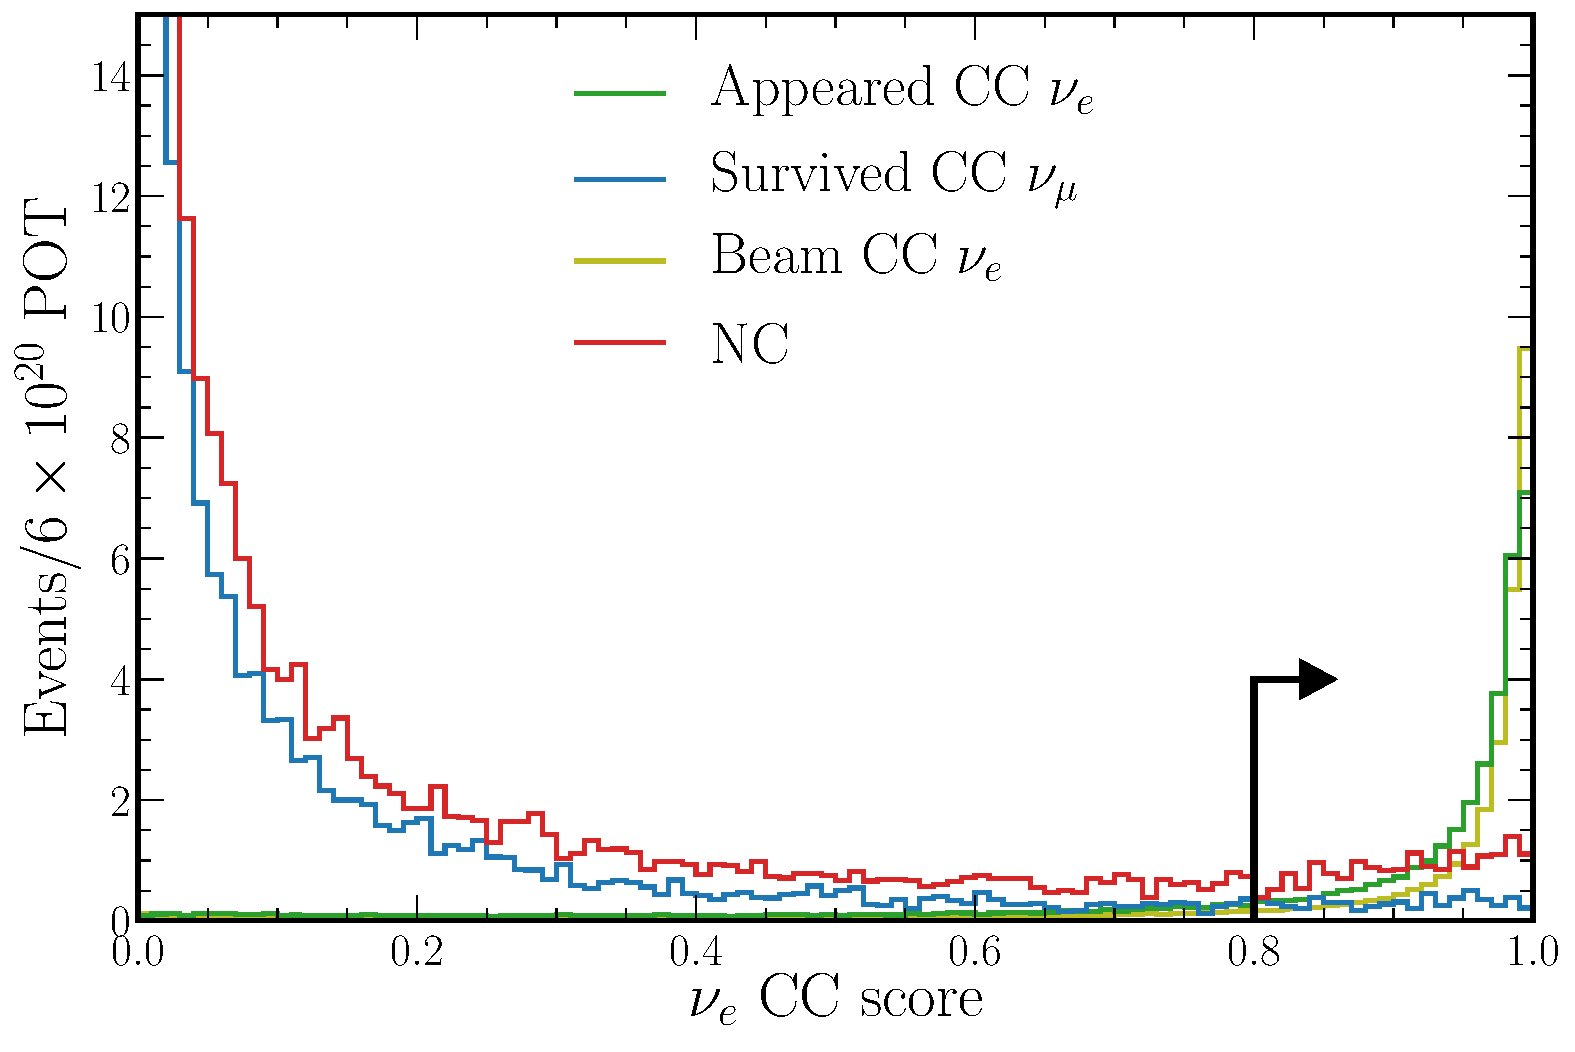
\includegraphics[width=0.7\textwidth]{diagrams/6-cvn/chipsnet/final_beam_nuel_outputs.pdf}
    \caption[Distribution of CC $\nu_{e}$ scores from the trained beam classification network.]
    {Distribution of CC $\nu_{e}$ scores for the different event categories. A score close to one
        signifies a CC $\nu_{e}$ like event. The y-axis has been truncated so that the CC
        $\nu_{\mu}$ and NC components are not fully visible in order to better show the
        distribution of signal events.}
    \label{fig:final_beam_nuel_outputs}
\end{figure}

The efficiency, purity, and their product for CC $\nu_{e}$ events (both appeared and beam) as a
function of selecting events above a certain CC $\nu_{e}$ score value is shown in
Fig.~\ref{fig:final_nuel_eff_curves}. The number of selected events for each event category and
corresponding signal efficiency and purity for the optimised figure-of-merit is shown in
Table.~\ref{tab:nuel_selection}. The figure-of-merit is optimised considering both appeared and
beam CC $\nu_{e}$ components as signal. Due to their indistinguishable nature, this is the only
approach that generates reasonable figure-of-merit cuts.

\begin{figure} % FINAL NUEL EFF CURVES DIAGRAM %
    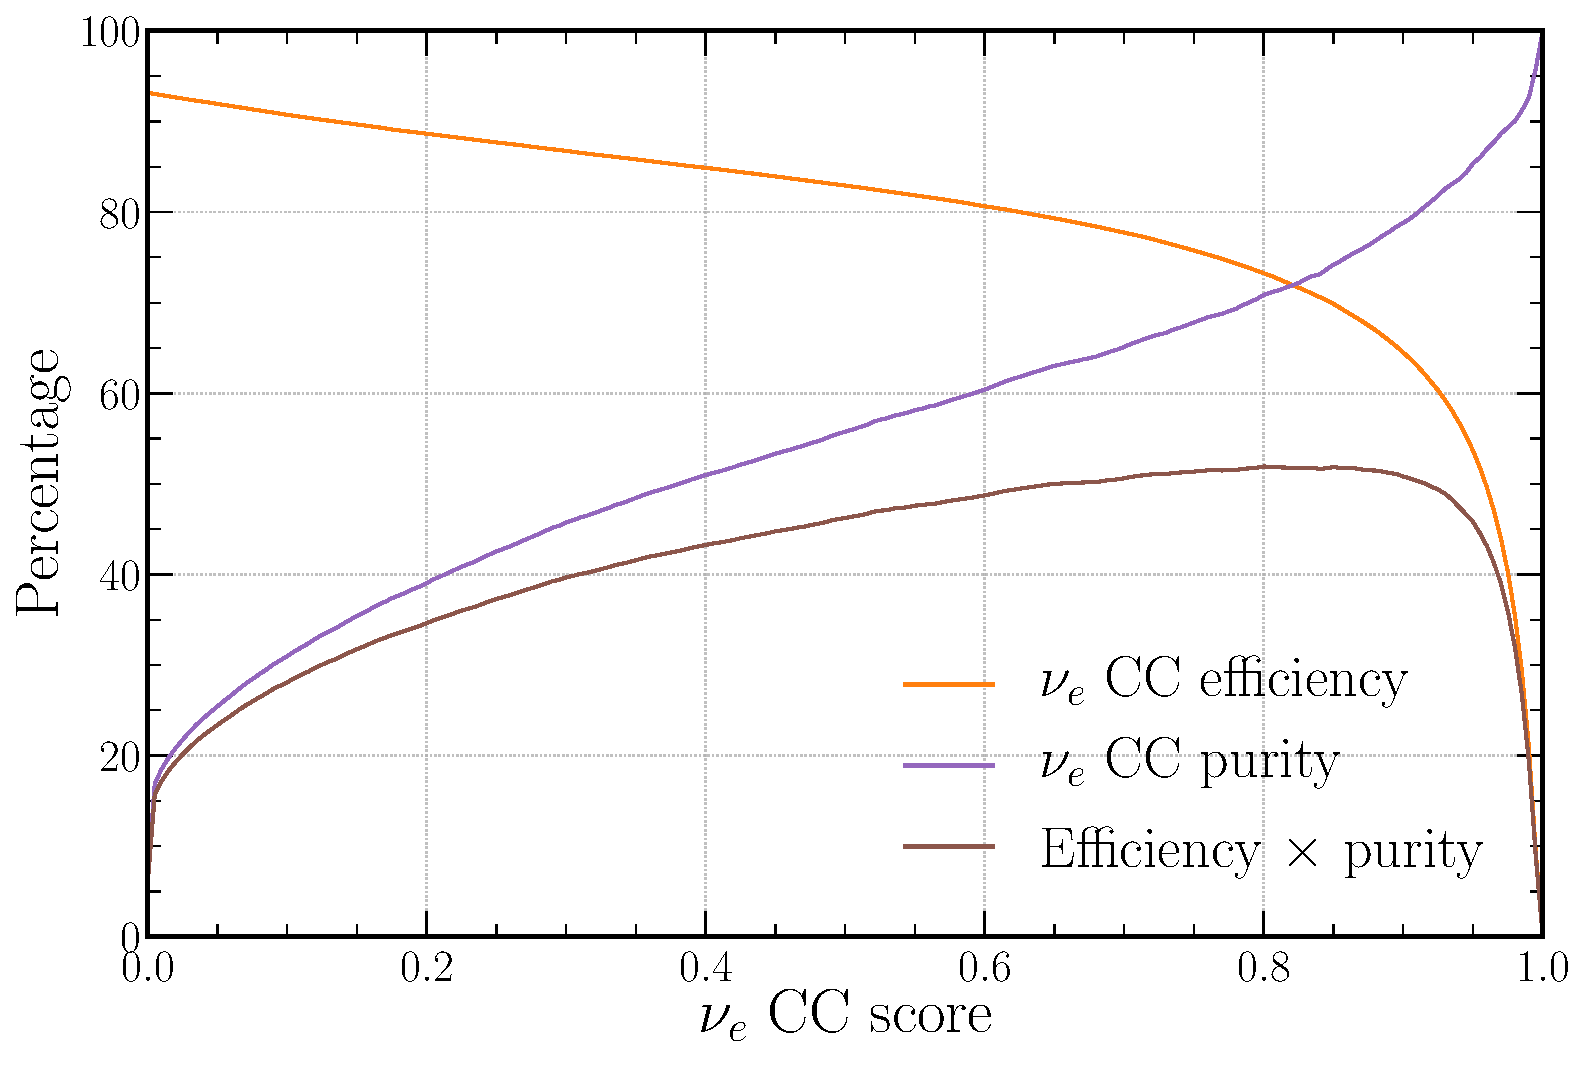
\includegraphics[width=0.7\textwidth]{diagrams/6-cvn/chipsnet/final_nuel_eff_curves.pdf}
    \caption[CC $\nu_{e}$ efficiency, purity and $\mathrm{efficiency}\times\mathrm{purity}$.]
    {CC $\nu_{e}$ efficiency, purity and $\mathrm{efficiency}\times\mathrm{purity}$ for different
        values of CC $\nu_{e}$ score selection. The maximum
        $\mathrm{efficiency}\times\mathrm{purity}$ value, the figure-of-merit, is found at a CC
        $\nu_{e}$ score of 0.8 as can be seen.}
    \label{fig:final_nuel_eff_curves}
\end{figure}

\begin{table}
    \begin{tabular}{ccccccc}
        Selection                               & Appeared CC $\nu_{e}$ & CC $\nu_{\mu}$ & Beam CC $\nu_{e}$ & NC    & Efficiency & Purity \\
        \midrule
        Pre+cos+esc                             & 40.8                  & 818.0          & 33.0              & 231.0 & 0.923      & 0.036  \\
        $\mathrm{eff}\times\mathrm{pur}$ (0.80) & 31.3                  & 6.1            & 26.7              & 17.6  & 0.708      & 0.383  \\
    \end{tabular}
    \caption[Table showing CC $\nu_{e}$ selected event numbers.]
    {Table showing CC $\nu_{e}$ selected event numbers for the various event categories as well as
        associated appeared CC $\nu_{e}$ efficiency and purity. Shown are the post preselection,
        `cosmic score' and `escapes score' numbers in addition to the two different
        figure-of-merit optimisations for which the CC $\nu_{e}$ score cut value is also given in
        brackets.}
    \label{tab:nuel_selection}
\end{table}

The CC $\nu_{e}$ selection efficiency for the $\mathrm{eff}\times\mathrm{pur}$ figure-of-merit as
a function of energy for the different event categories is shown in
Fig.~\ref{fig:final_nuel_hists}. From low neutrino energies, both CC $\nu_{e}$ category selection
efficiencies rise steeply to a plateau of 80\% beginning at \unit{4}{GeV}. This is expected as low
energy CC $\nu_{e}$ events typically do not have well-defined electron Cherenkov rings, leading to
their rejection. Due to the abundance of selected intrinsic beam CC $\nu_{e}$ events at higher
energies the appeared CC $\nu_{e}$ purity is observed to peak at approximately \unit{2.5}{\GeV}
before declining. The NC efficiency is seen to slowly increase approaching 15\% for hadronic
system energies above \unit{5}{\GeV}; this is likely due to high energy pions or protons being
misidentified as electrons. Importantly, however, within the key signal region from 2 to
\unit{4}{\GeV}, NC selection efficiency remains low.

\begin{figure} % FINAL NUEL HISTS DIAGRAM %
    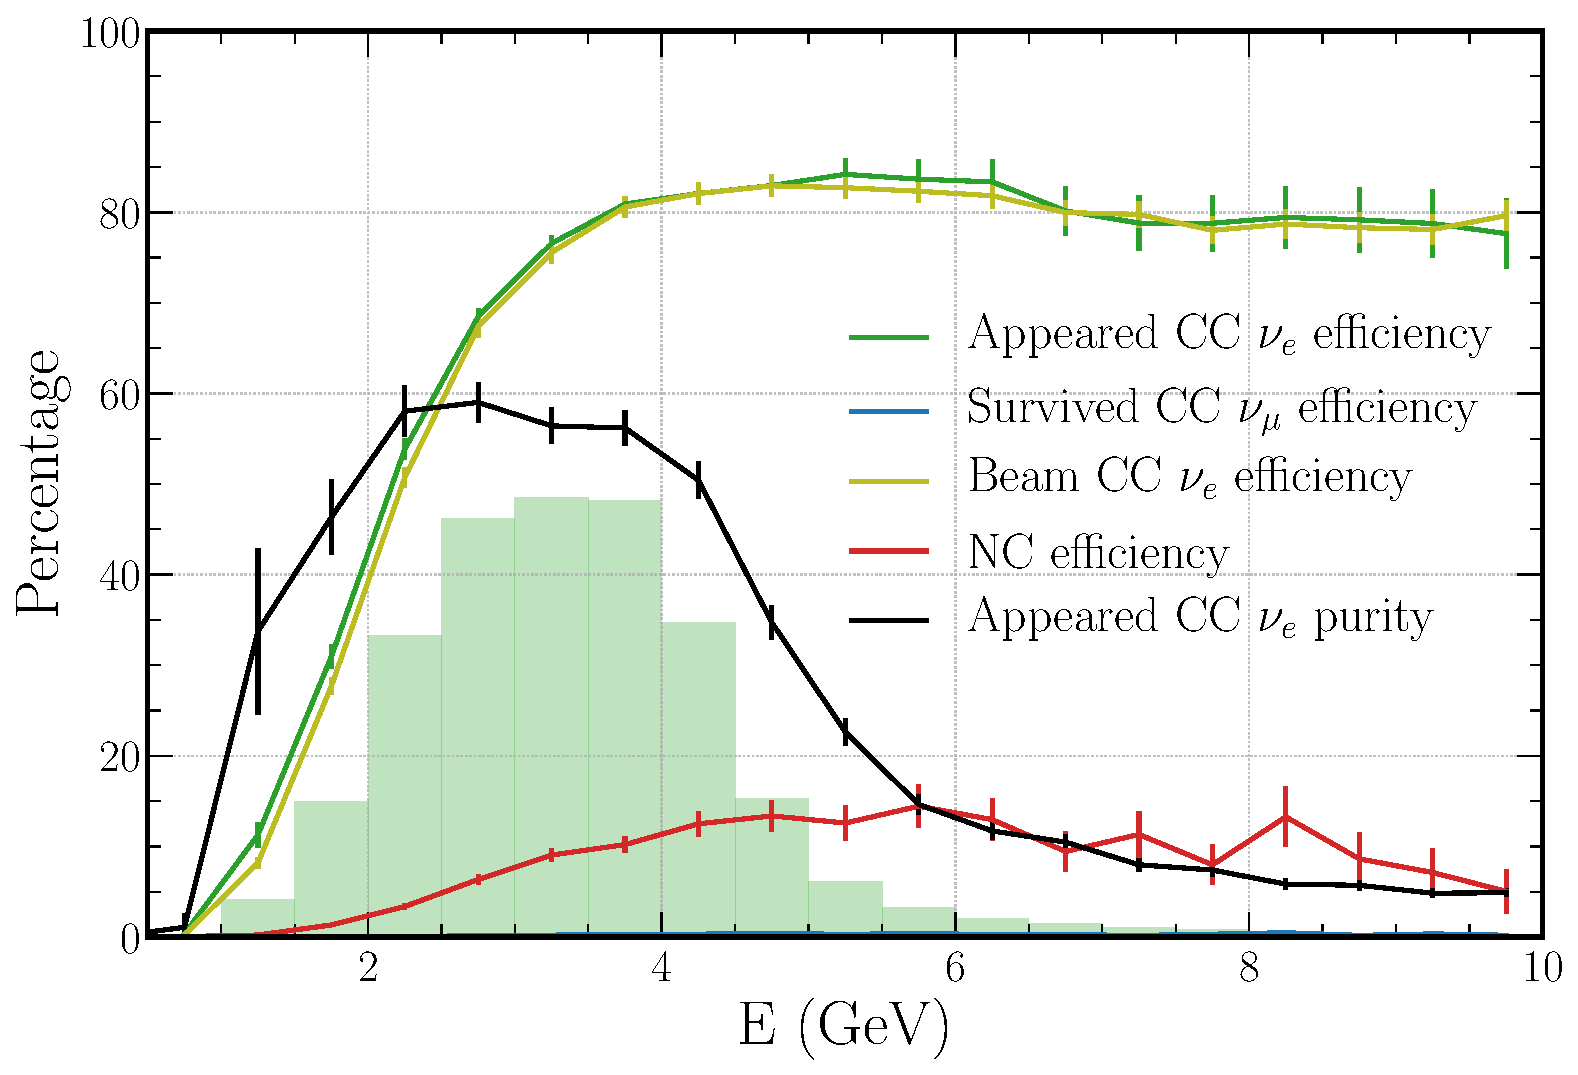
\includegraphics[width=0.7\textwidth]{diagrams/6-cvn/chipsnet/final_nuel_hists.pdf}
    \caption[Efficiency of CC $\nu_{e}$ selection as a function of energy.]
    {Efficiency of CC $\nu_{e}$ selection for the different event categories as well as appeared
        CC $\nu_{e}$ purity as a function of neutrino energy. The true appeared CC $\nu_{e}$
        neutrino energy distribution is shown in the green. All CC categories are shown in terms
        of neutrino energy, while NC events are shown in terms of the hadronic energy.}
    \label{fig:final_nuel_hists}
\end{figure}

\subsubsection*{CC $\nu_{\mu}$ selection} %%%%%%%%%%%%%%%%%%%%%%%%%%%%%%%%%%%%%%%%%%%%%%%%%%%%%%%%

The distribution of CC $\nu_{\mu}$ scores for the different event categories is shown in
Fig.~\ref{fig:final_beam_numu_outputs}. Excellent separation between appeared CC $\nu_{\mu}$
signal and both CC $\nu_{e}$ components and NC background is achieved. For high CC $\nu_{\mu}$
scores the difference between signal and background event counts is approximately three orders of
magnitude.

\begin{figure} % BEAM OUTPUTS NUMU DIAGRAM %
    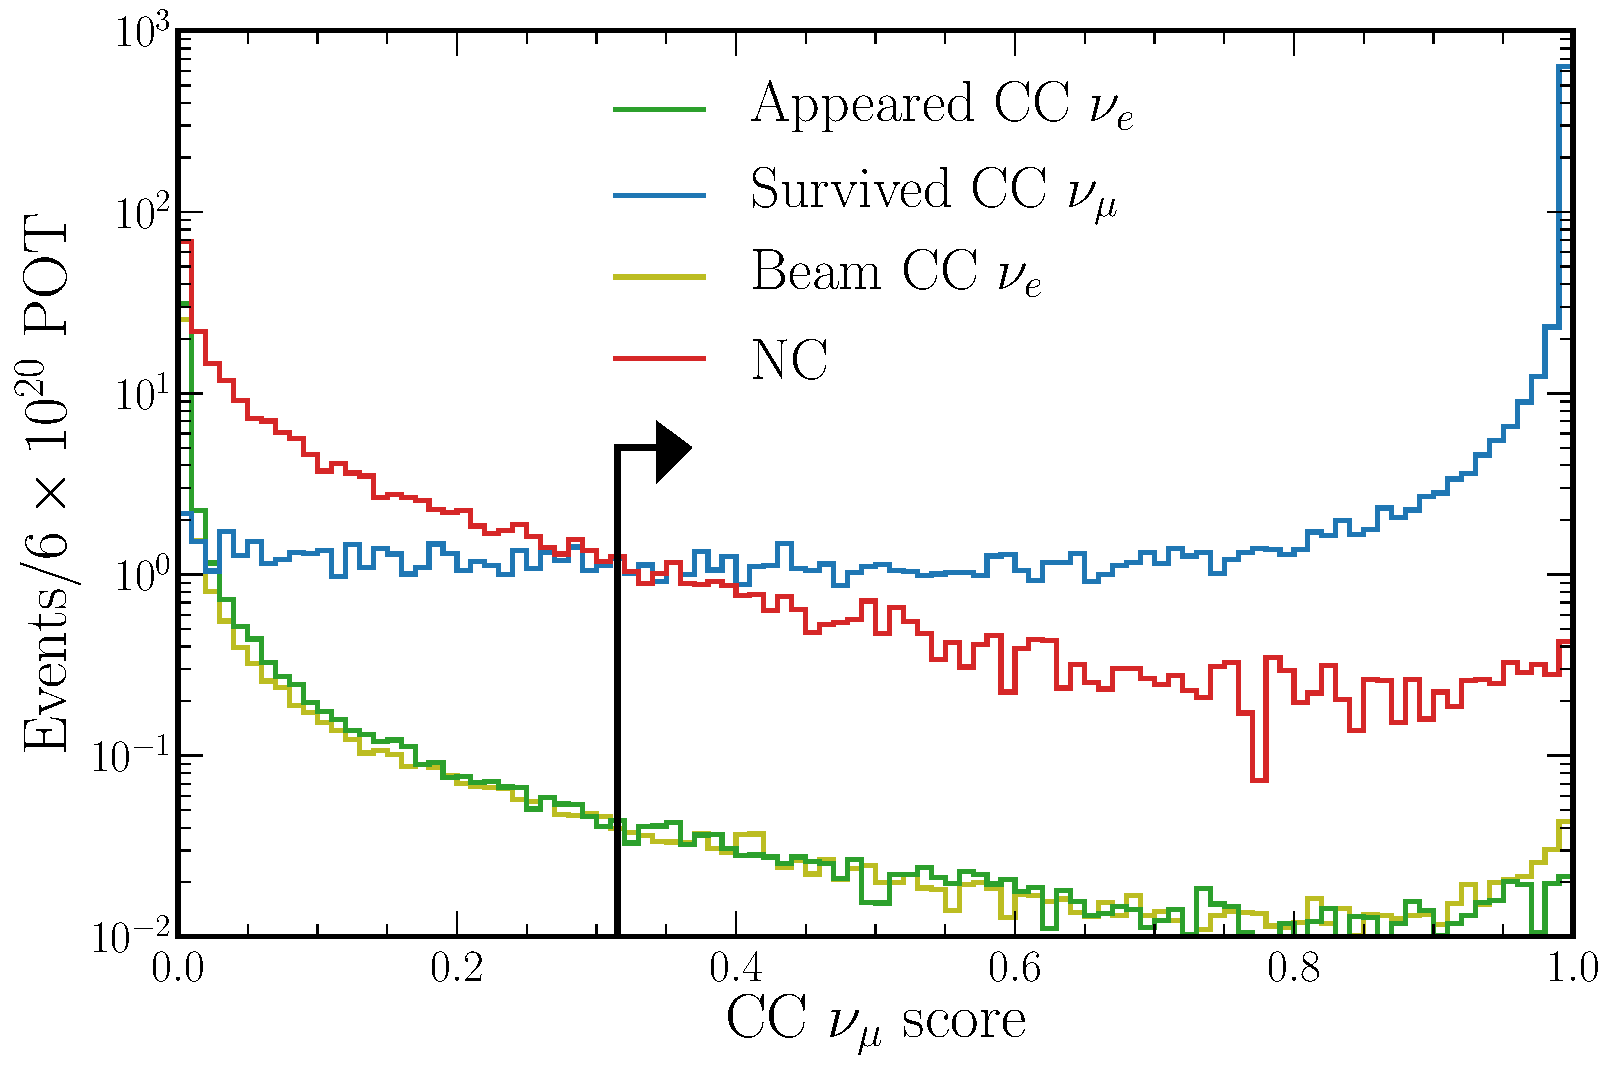
\includegraphics[width=0.7\textwidth]{diagrams/6-cvn/chipsnet/final_beam_numu_outputs.pdf}
    \caption[Distribution of CC $\nu_{\mu}$ scores from the trained beam classification network.]
    {Distribution of CC $\nu_{\mu}$ scores for the different event categories. A score close to
        one signifies a CC $\nu_{\mu}$ like event.}
    \label{fig:final_beam_numu_outputs}
\end{figure}

The efficiency, purity, and their product for survived CC $\nu_{\mu}$ events as a function of
selecting events above a certain CC $\nu_{\mu}$ score value is shown in
Fig.~\ref{fig:final_numu_eff_curves}. The number of selected events for each event category and
corresponding signal efficiency and purity for both optimised figure-of-merits is shown in
Table.~\ref{tab:numu_selection}. An incredibly high signal purity of 99.9\% is achieved using the
$s/\sqrt{b}$ figure-of-merit selection. Although the final selection efficiency is low for both
figure-of-merit optimisations, this is desirable to ensure events are fully contained for energy
estimation. When considering just the CC $\nu_{\mu}$ events for which the primary charged muon
is contained, an 87\% selection efficiency for the first figure-of-merit is achieved.

\begin{figure} % FINAL NUMU EFF CURVES DIAGRAM %
    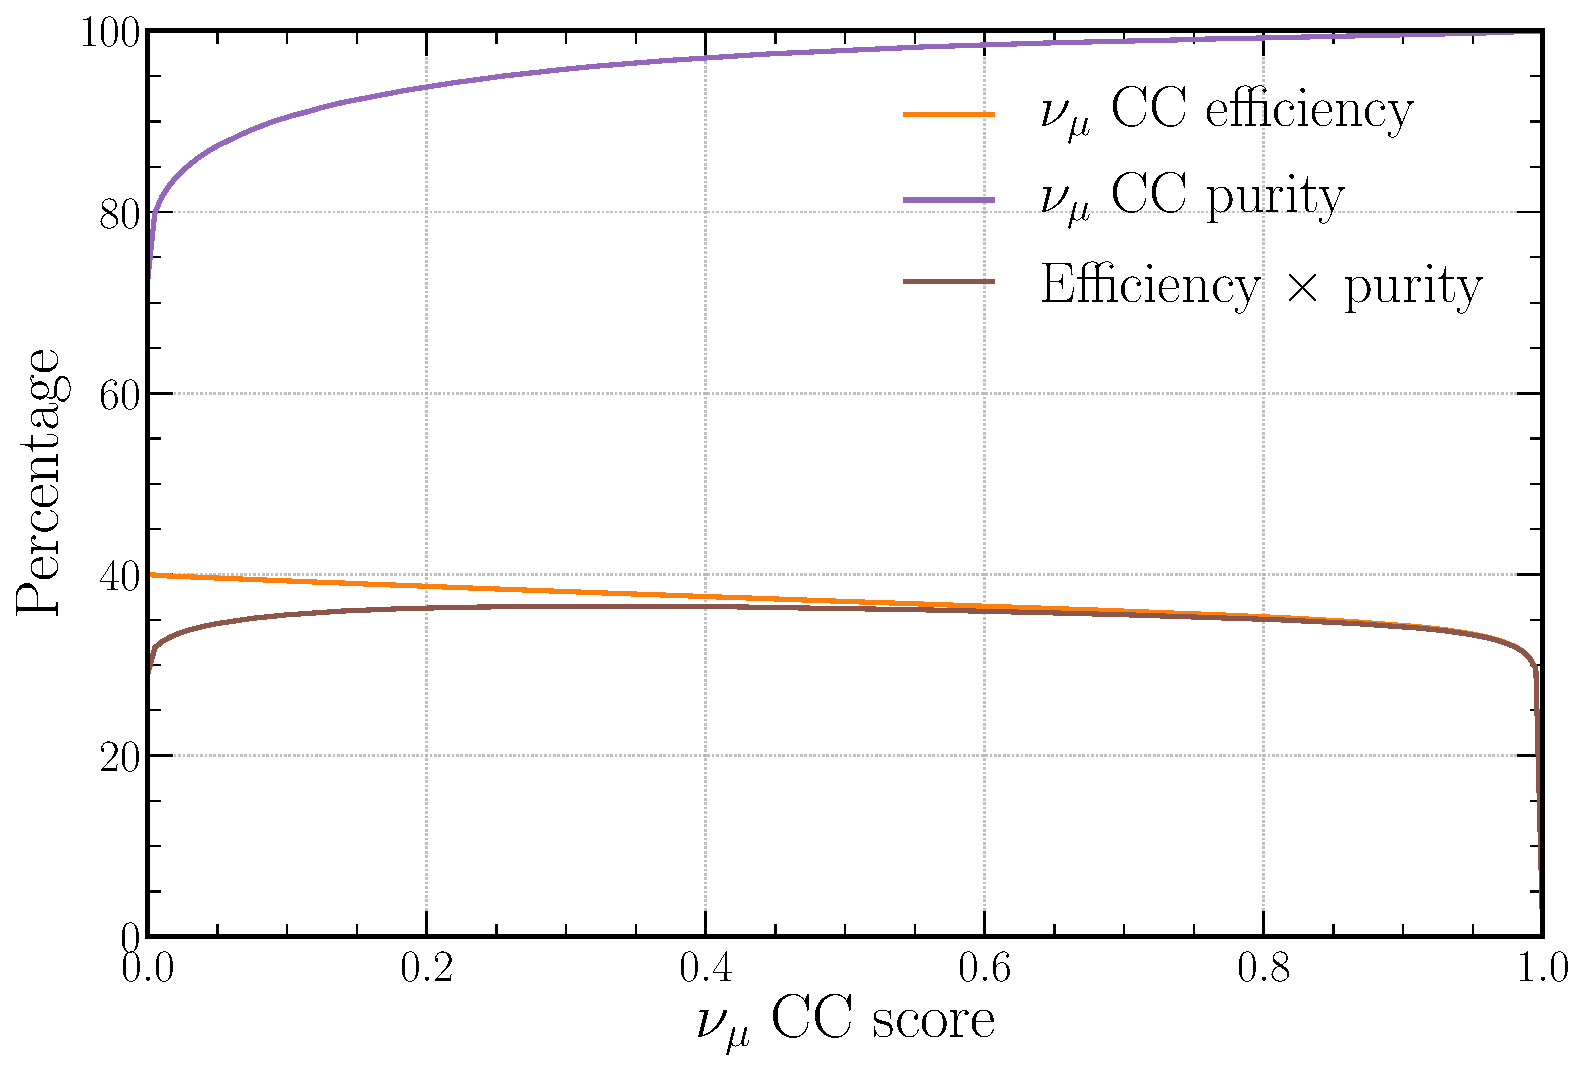
\includegraphics[width=0.7\textwidth]{diagrams/6-cvn/chipsnet/final_numu_eff_curves.pdf}
    \caption[CC $\nu_{\mu}$ efficiency, purity and $\mathrm{efficiency}\times\mathrm{purity}$.]
    {CC $\nu_{\mu}$ efficiency, purity and $\mathrm{efficiency}\times\mathrm{purity}$ for
        different values of CC $\nu_{\mu}$ score selection. The maximum
        $\mathrm{efficiency}\times\mathrm{purity}$ value, the first of the two figure-of-merits,
        is found at a CC $\nu_{\mu}$ score of 0.315 as can be seen.}
    \label{fig:final_numu_eff_curves}
\end{figure}

\begin{table}
    \begin{tabular}{ccccccc}
        Selection                                & CC $\nu_{\mu}$ & Appeared CC $\nu_{e}$ & Beam CC $\nu_{e}$ & NC    & Efficiency & Purity \\
        \midrule
        Pre+cos+esc                              & 818.0          & 40.8                  & 33.0              & 231.0 & 0.400      & 0.729  \\
        \midrule
        $\mathrm{eff}\times\mathrm{pur}$ (0.315) & 777.9          & 1.32                  & 1.37              & 29.3  & 0.380      & 0.961  \\
        $s/\sqrt{b}$ (0.995)                     & 605.9          & 0.01                  & 0.03              & 0.25  & 0.296      & 0.999  \\
    \end{tabular}
    \caption[Table showing CC $\nu_{\mu}$ selected event numbers.]
    {Table showing CC $\nu_{\mu}$ selected event numbers for the various event categories as well
        as associated appeared CC $\nu_{\mu}$ efficiency and purity. Shown are the post
        preselection, `cosmic score' and `escapes score' numbers in addition to the two different
        figure-of-merit optimisations for which the CC $\nu_{\mu}$ score cut value is given in
        brackets.}
    \label{tab:numu_selection}
\end{table}

The CC $\nu_{\mu}$ selection efficiency for the $\mathrm{eff}\times\mathrm{pur}$ figure-of-merit
as a function of energy for the different event categories is shown in
Fig.~\ref{fig:final_numu_hists}. Survived CC $\nu_{\mu}$ selection efficiency peaks just below
\unit{2}{\GeV} before slowly declining, this is entirely explained by higher energy events being
less likely to have their primary charged muon fully contained within the detector. The signal
purity is observed to remain very high (>95\%) across the main signal energy region. As in the CC
$\nu_{e}$ selection case the NC efficiency is seen to rise with energy, again likely due to
misidentification of energetic protons and pions.

\begin{figure} % FINAL NUMU HISTS DIAGRAM %
    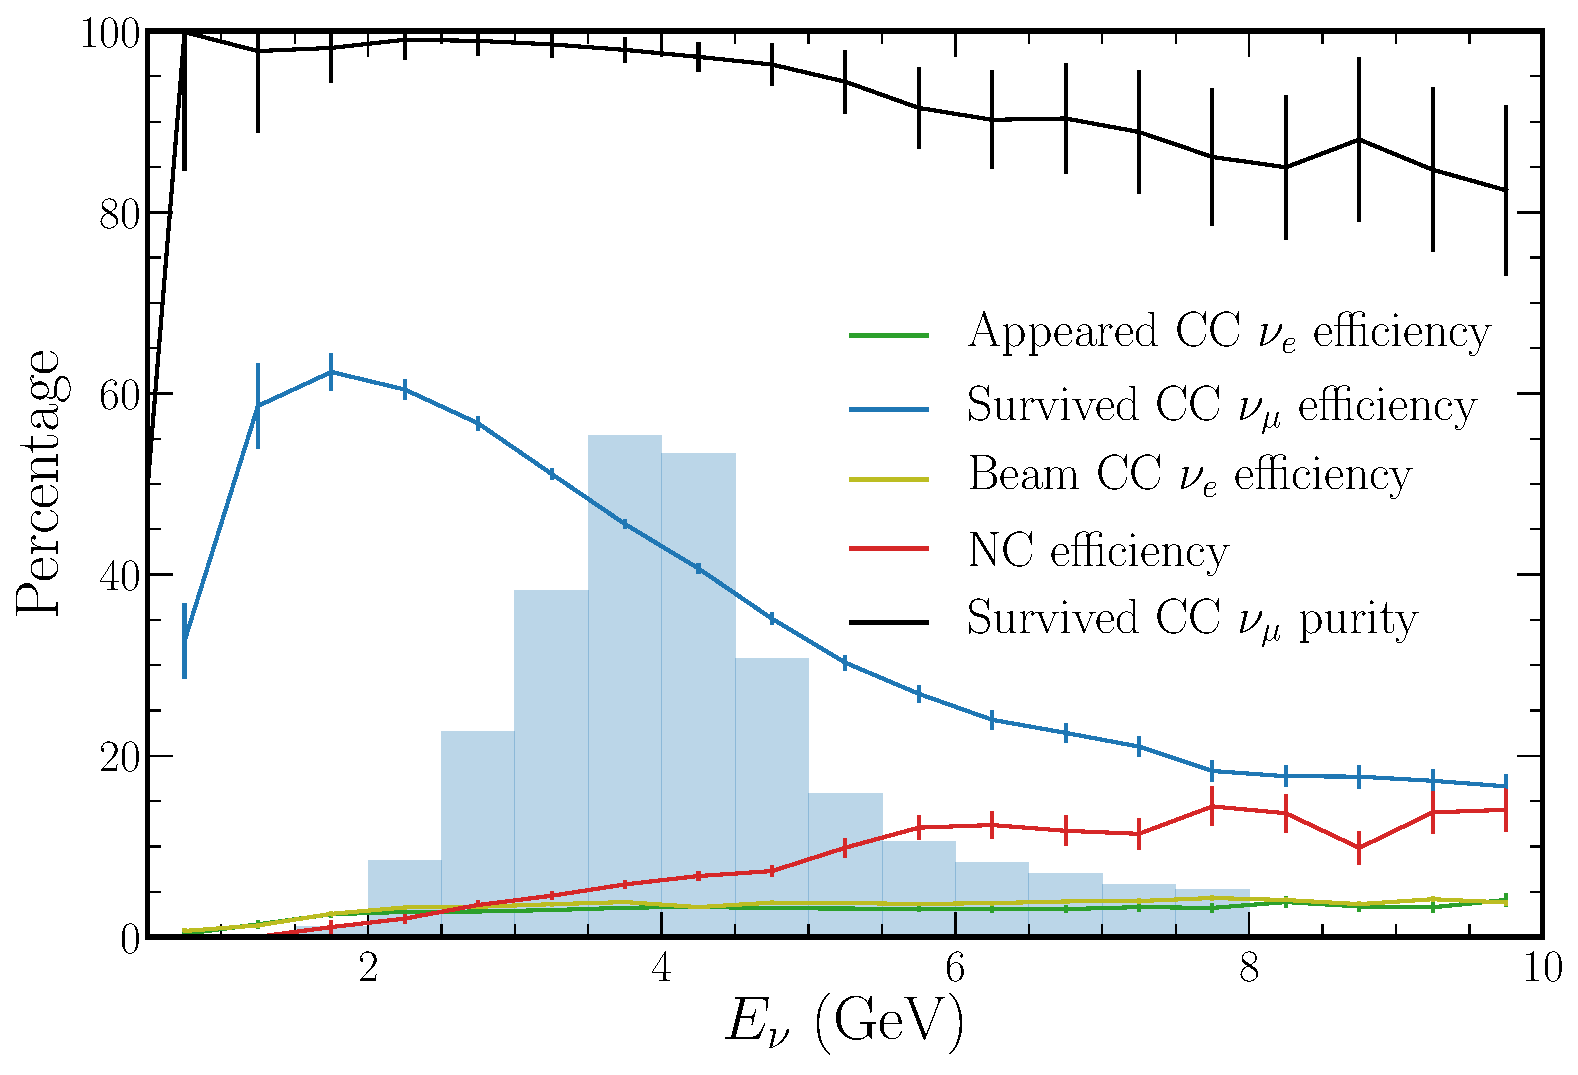
\includegraphics[width=0.7\textwidth]{diagrams/6-cvn/chipsnet/final_numu_hists.pdf}
    \caption[Efficiency of CC $\nu_{\mu}$ selection as a function of energy.]
    {Efficiency of CC $\nu_{\mu}$ selection for the different event categories as well as survived
        CC $\nu_{\mu}$ purity as a function of neutrino energy. The true survived CC $\nu_{\mu}$
        neutrino energy distribution is shown in the blue. All CC categories are shown in terms of
        neutrino energy, while NC events are shown in terms of the hadronic energy.}
    \label{fig:final_numu_hists}
\end{figure}

\subsubsection*{Interaction type classification} %%%%%%%%%%%%%%%%%%%%%%%%%%%%%%%%%%%%%%%%%%%%%%%%%

Using the `CC category' output from the trained beam classification network, the CC interaction
type for CC $\nu_{e}$ and CC $\nu_{\mu}$ selected events is also determined. As in the `combined
category' output case the highest-scoring neuron can be used for classification. The resulting
classification matrix is shown in Fig.~\ref{fig:final_cc_cat_confusion}.

- As the different final states will have different energy resolutions and sytematic
uncertainties, it may be possible for a future analysis to improve the oscillation paramter
sensitivity by indentifying subsamples with specific topologies.

\begin{figure} % FINAL CC CAT CONFUSION DIAGRAM %
    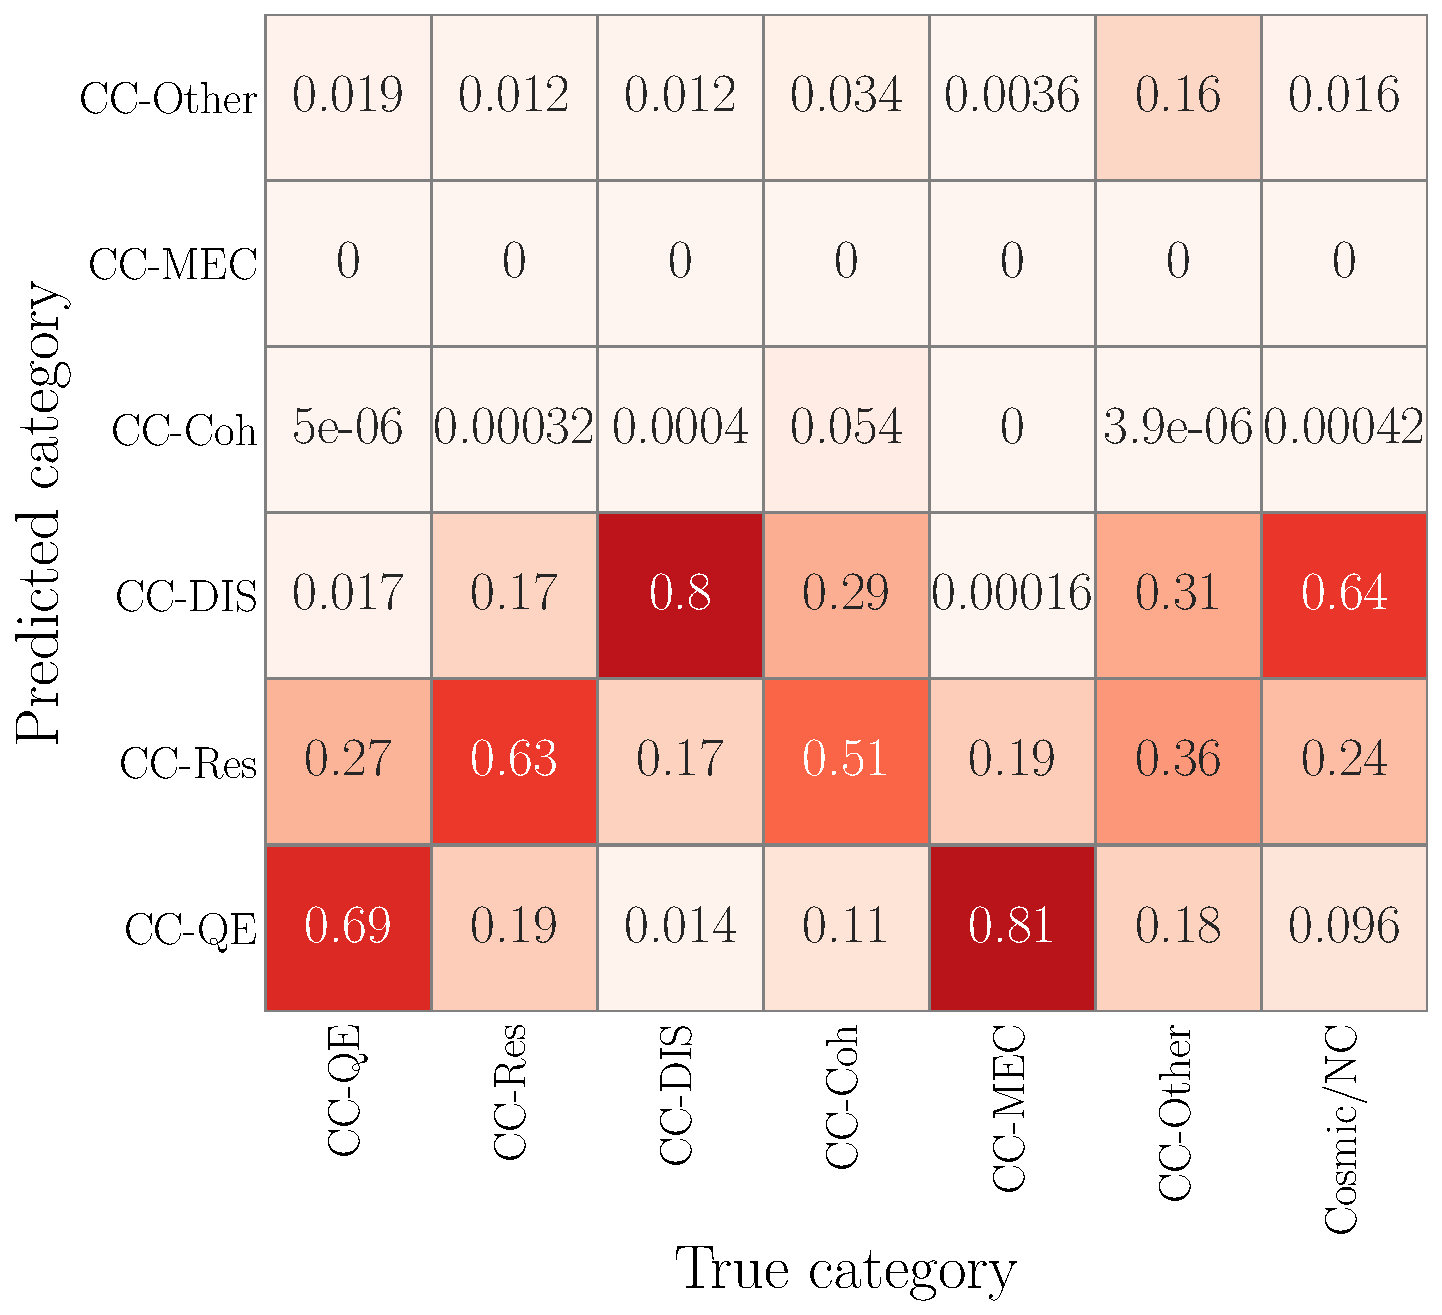
\includegraphics[width=0.7\textwidth]{diagrams/6-cvn/chipsnet/final_cc_cat_confusion.pdf}
    \caption[Classification matrix for the `CC category' output of the beam classification
        network.] {Classification matrix for the `CC category' output of the trained beam
        classification network applied to the evaluation sample. The numbers shown are the
        fraction of true category events that are classified into each of the three possible
        categories.}
    \label{fig:final_cc_cat_confusion}
\end{figure}

- This classification is then used during energy estimation discussed in the following section!

\begin{figure} % FINAL NC CAT CONFUSION DIAGRAM %
    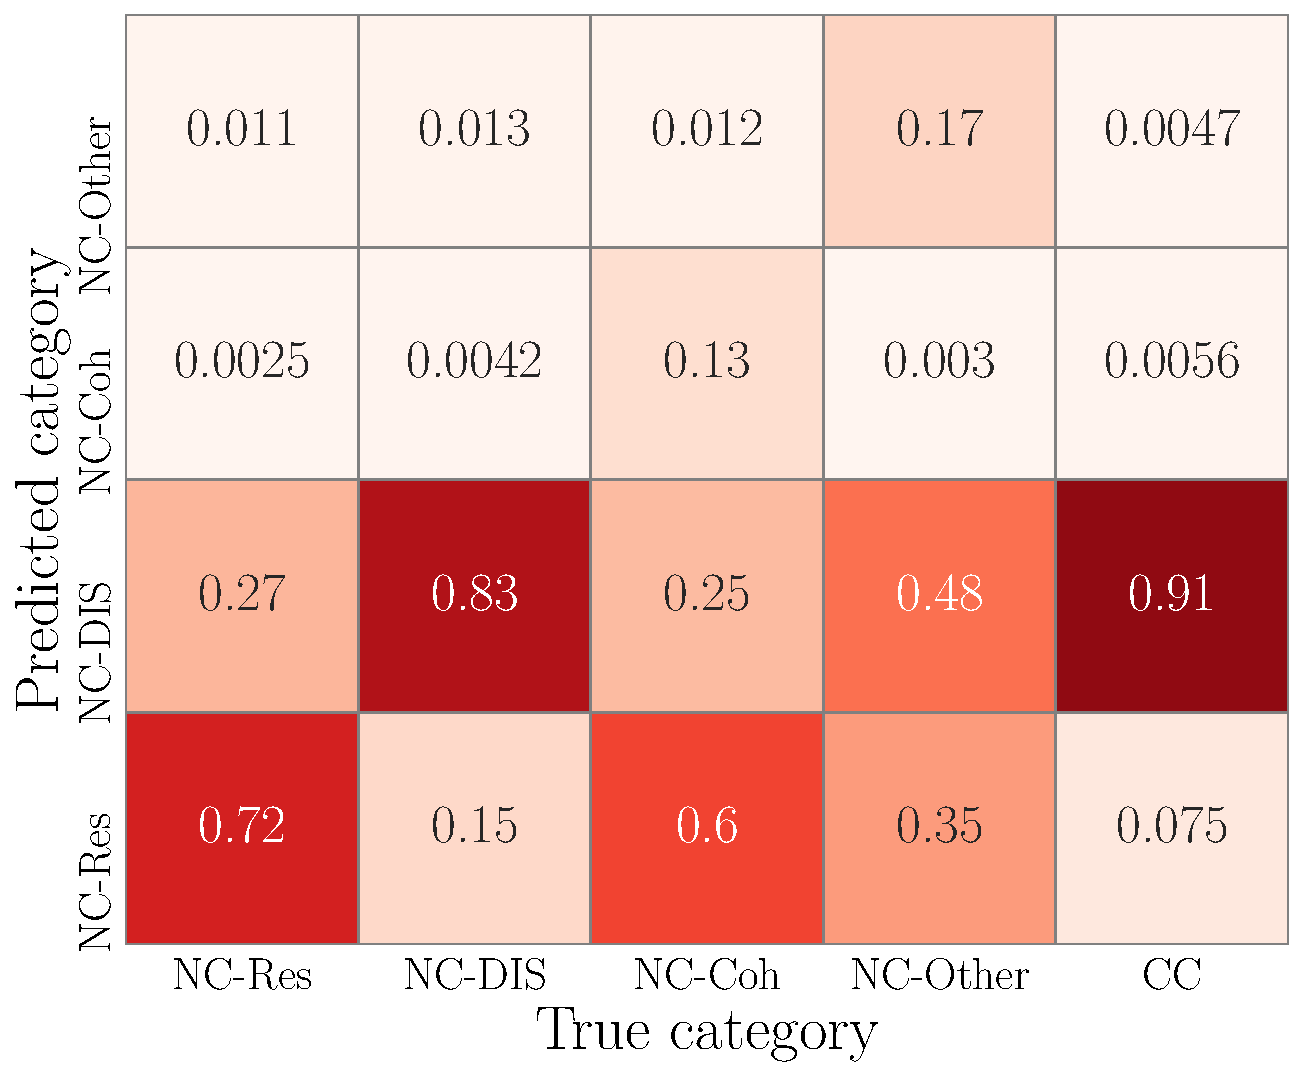
\includegraphics[width=0.7\textwidth]{diagrams/6-cvn/chipsnet/final_nc_cat_confusion.pdf}
    \caption[final nc cat confusion short]
    {final nc cat confusion long}
    \label{fig:final_nc_cat_confusion}
\end{figure}

\subsubsection*{Primary particle counting} %%%%%%%%%%%%%%%%%%%%%%%%%%%%%%%%%%%%%%%%%%%%%%%%%%%%%%%

- Primary partile scores can be combined to give compounded scores for the exclusive final state
selections.
- Don't look at this in this work, just use the fact it increases primary task performance.

\subsection{Energy estimation} %%%%%%%%%%%%%%%%%%%%%%%%%%%%%%%%%%%%%%%%%%%%%%%%%%%%%%%%%%%%%%%%%%%
\label{sec:cvn_results_energy} %%%%%%%%%%%%%%%%%%%%%%%%%%%%%%%%%%%%%%%%%%%%%%%%%%%%%%%%%%%%%%%%%%%

- Should really have used a uniform sample for training
- Need to mention why we still use dropout!

\begin{figure} % FINAL ENERGY DISTS DIAGRAM %
    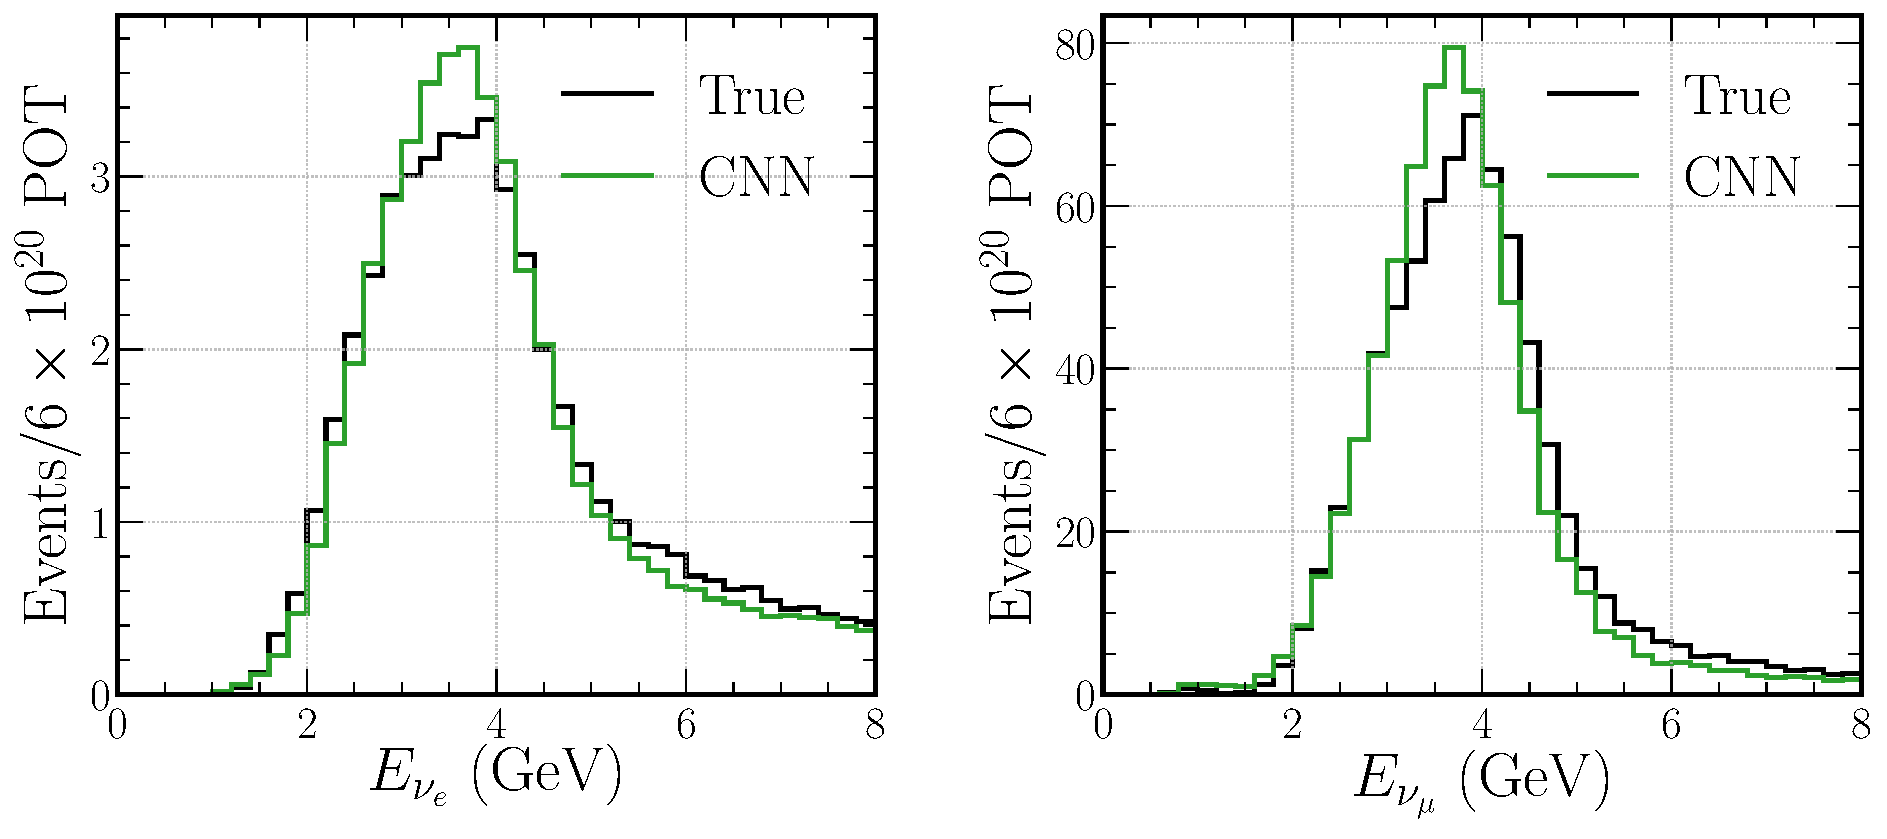
\includegraphics[width=0.7\textwidth]{diagrams/6-cvn/chipsnet/final_energy_dists.pdf}
    \caption[final energy dists short]
    {final energy dist long}
    \label{fig:final_energy_dists}
\end{figure}

\begin{figure} % FINAL ENERGY FRAC DIAGRAM %
    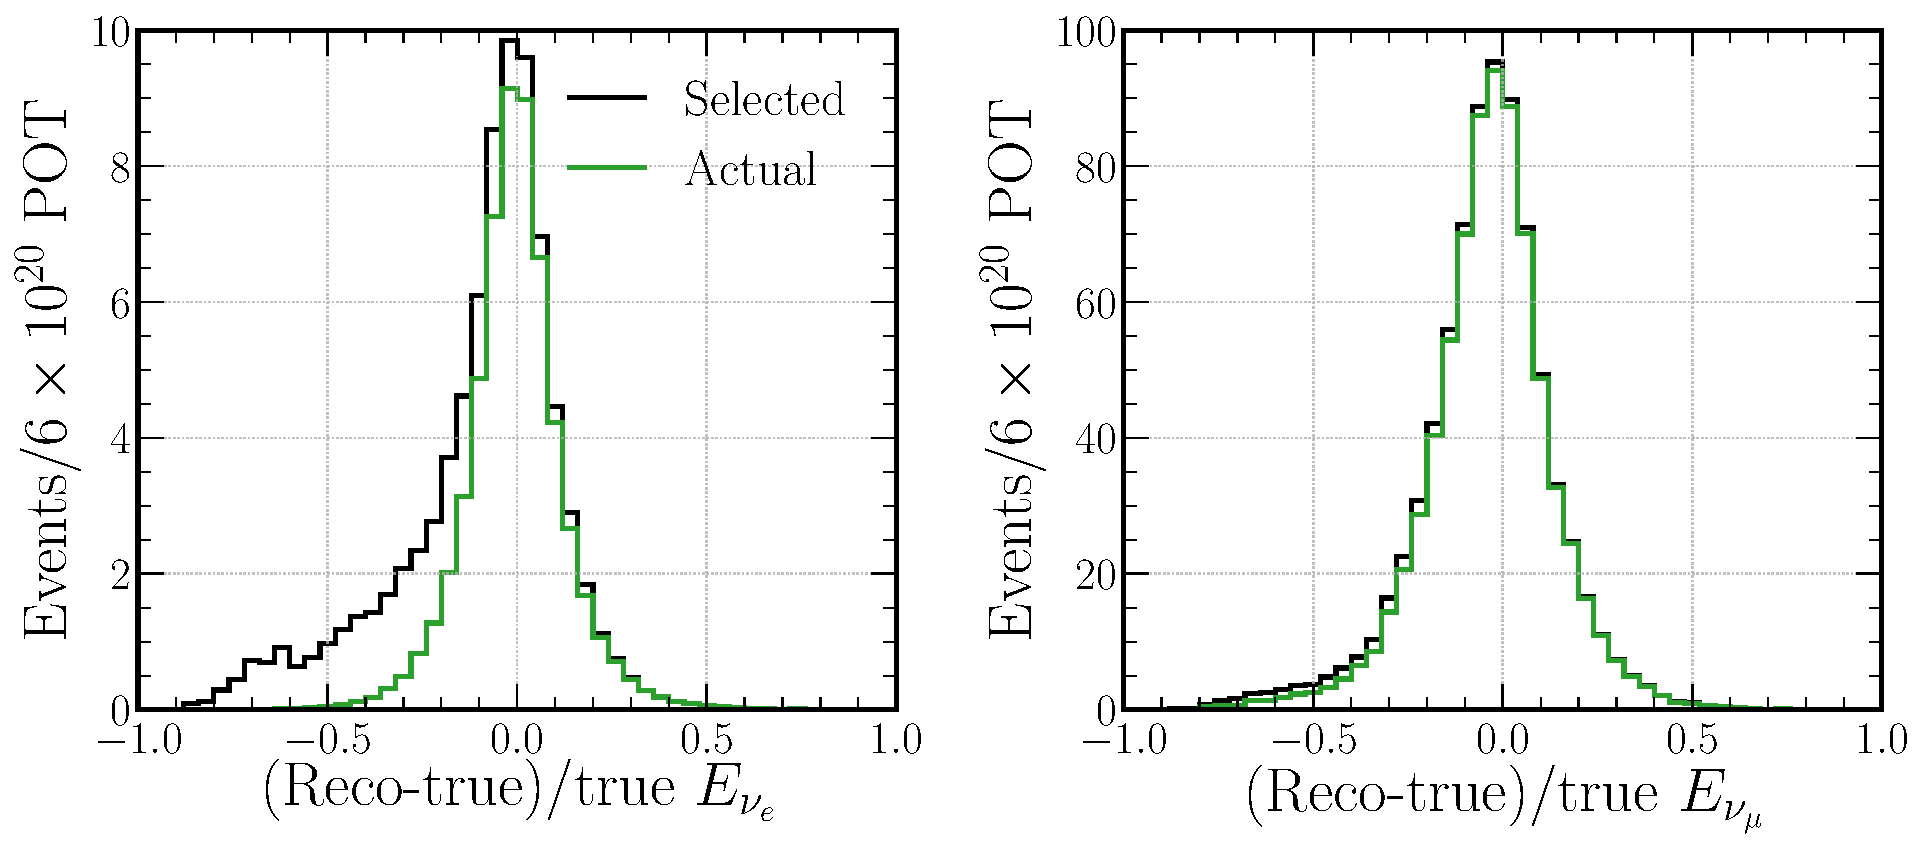
\includegraphics[width=0.7\textwidth]{diagrams/6-cvn/chipsnet/final_energy_frac.pdf}
    \caption[final energy frac short]
    {final energy frac long}
    \label{fig:final_energy_frac}
\end{figure}

\begin{figure} % FINAL ENERGY FRAC SPLIT DIAGRAM %
    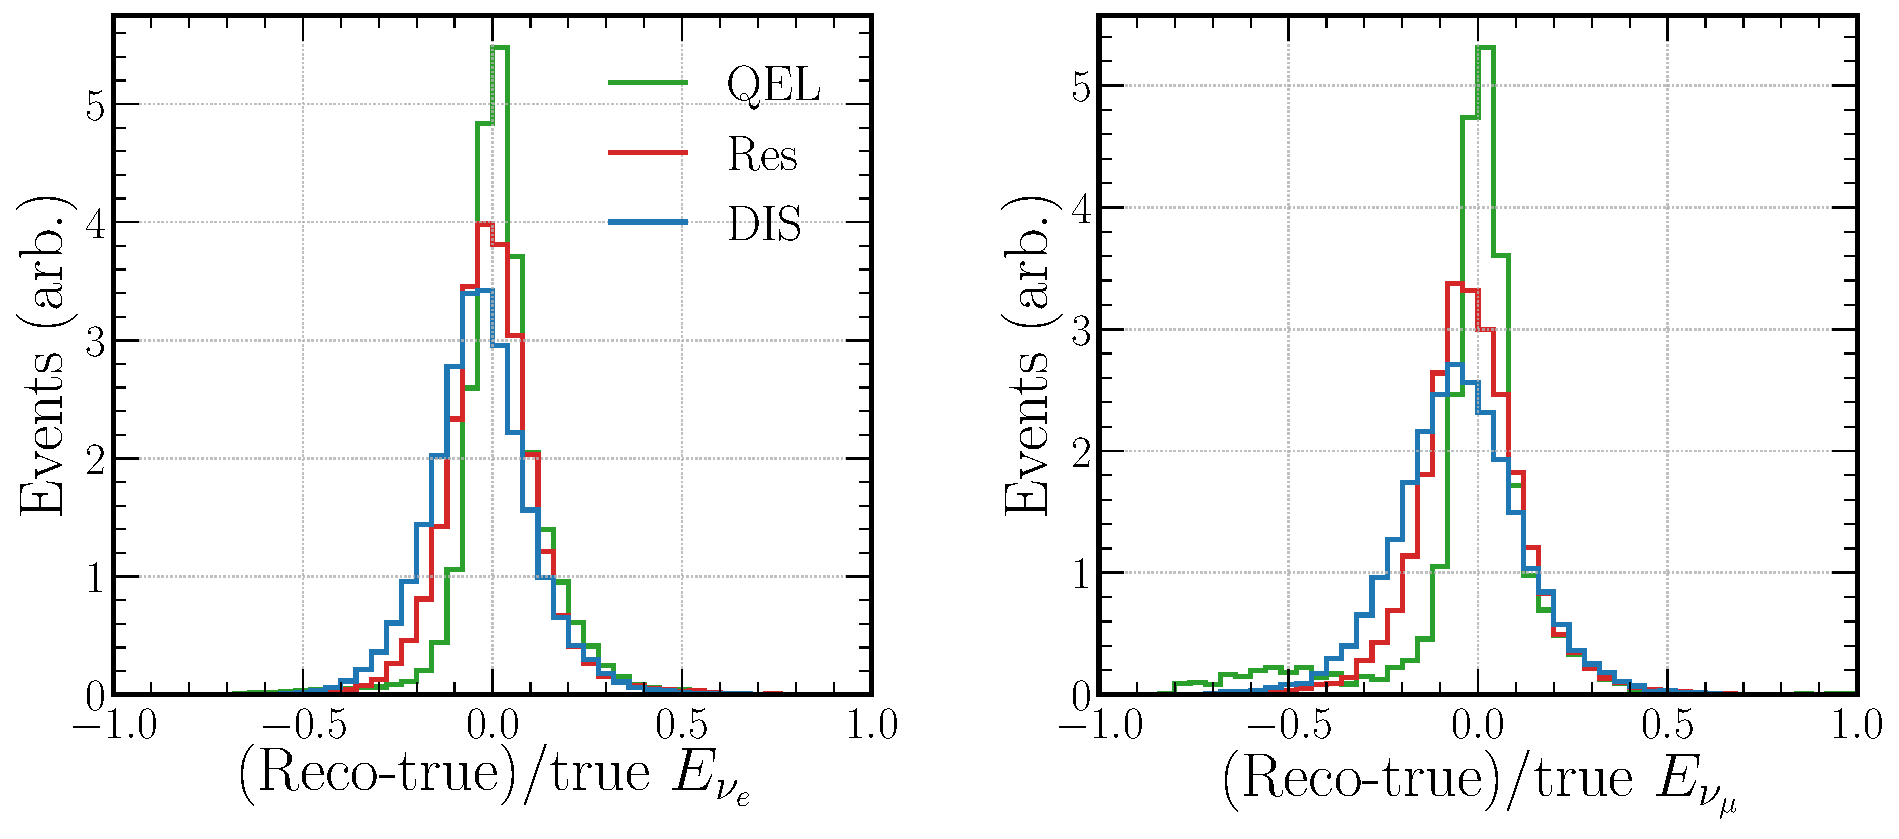
\includegraphics[width=0.7\textwidth]{diagrams/6-cvn/chipsnet/final_energy_frac_split.pdf}
    \caption[final energy frac split short]
    {final energy frac split long}
    \label{fig:final_energy_frac_split}
\end{figure}

\begin{figure} % FINAL 2D ENERGY DIAGRAM %
    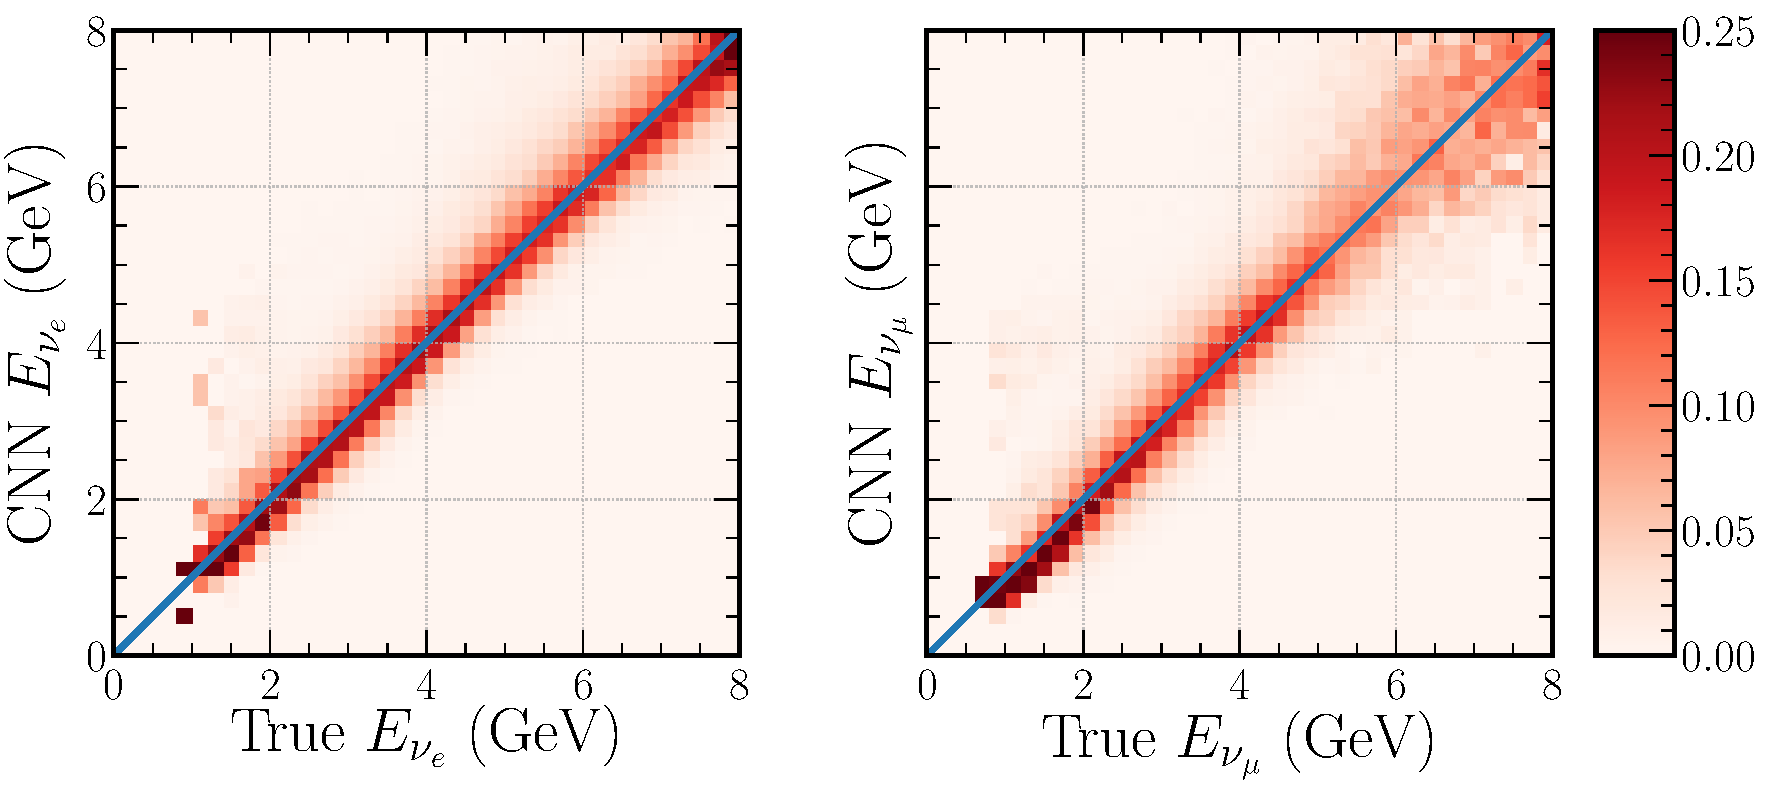
\includegraphics[width=0.7\textwidth]{diagrams/6-cvn/chipsnet/final_energy_2d.pdf}
    \caption[final energy 2d short]
    {final energy 2d long}
    \label{fig:final_energy_2d}
\end{figure}

\begin{figure} % FINAL 2D ENERGY DIAGRAM %
    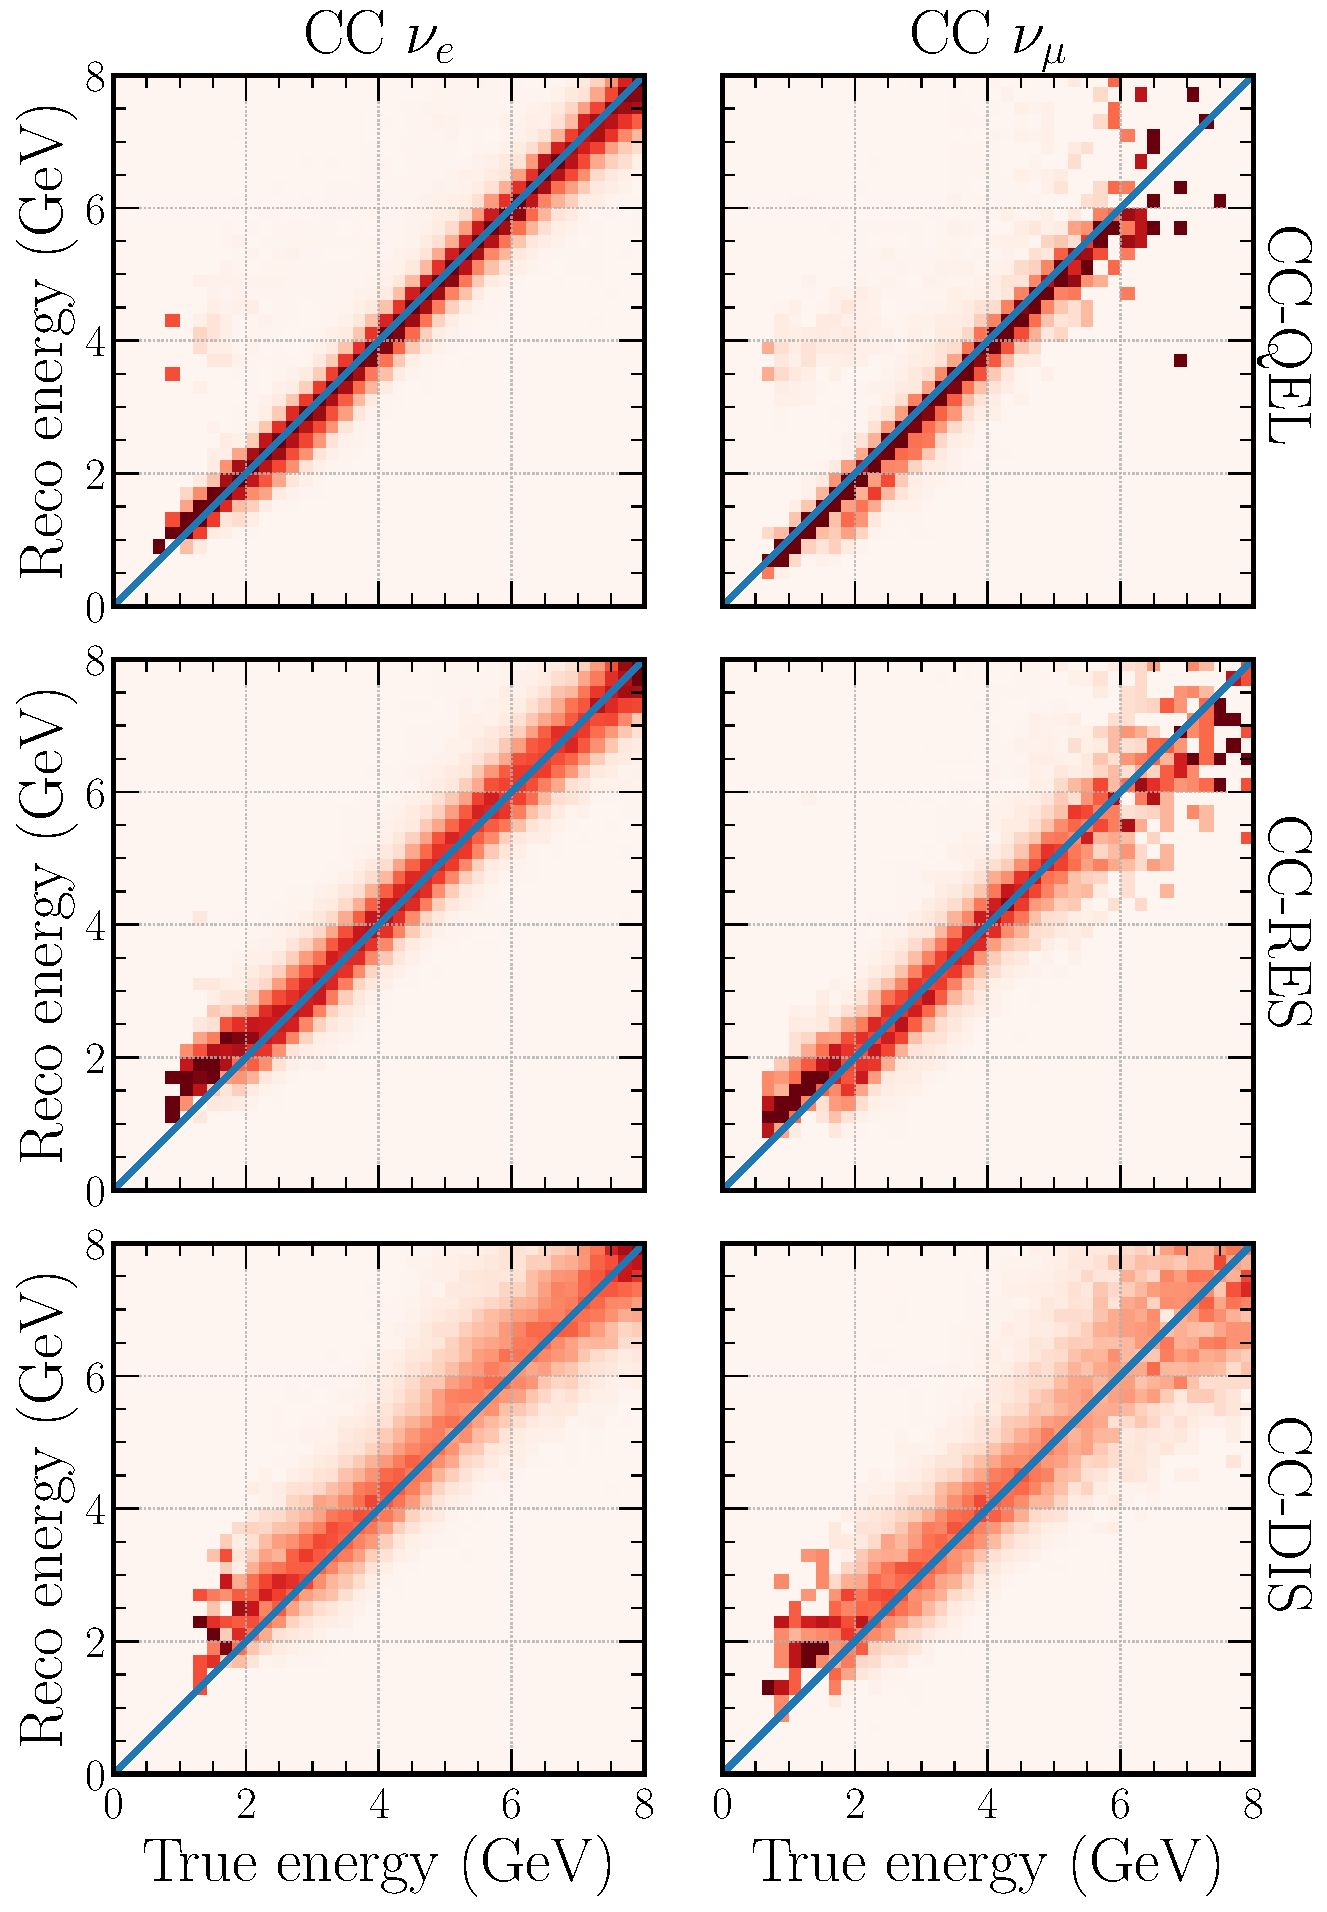
\includegraphics[width=0.7\textwidth]{diagrams/6-cvn/chipsnet/final_energy_2d_cats.pdf}
    \caption[final energy 2d cats short]
    {final energy 2d cats long}
    \label{fig:final_energy_2d_cats}
\end{figure}

\begin{figure} % FINAL NUEL ENERGY DIAGRAM %
    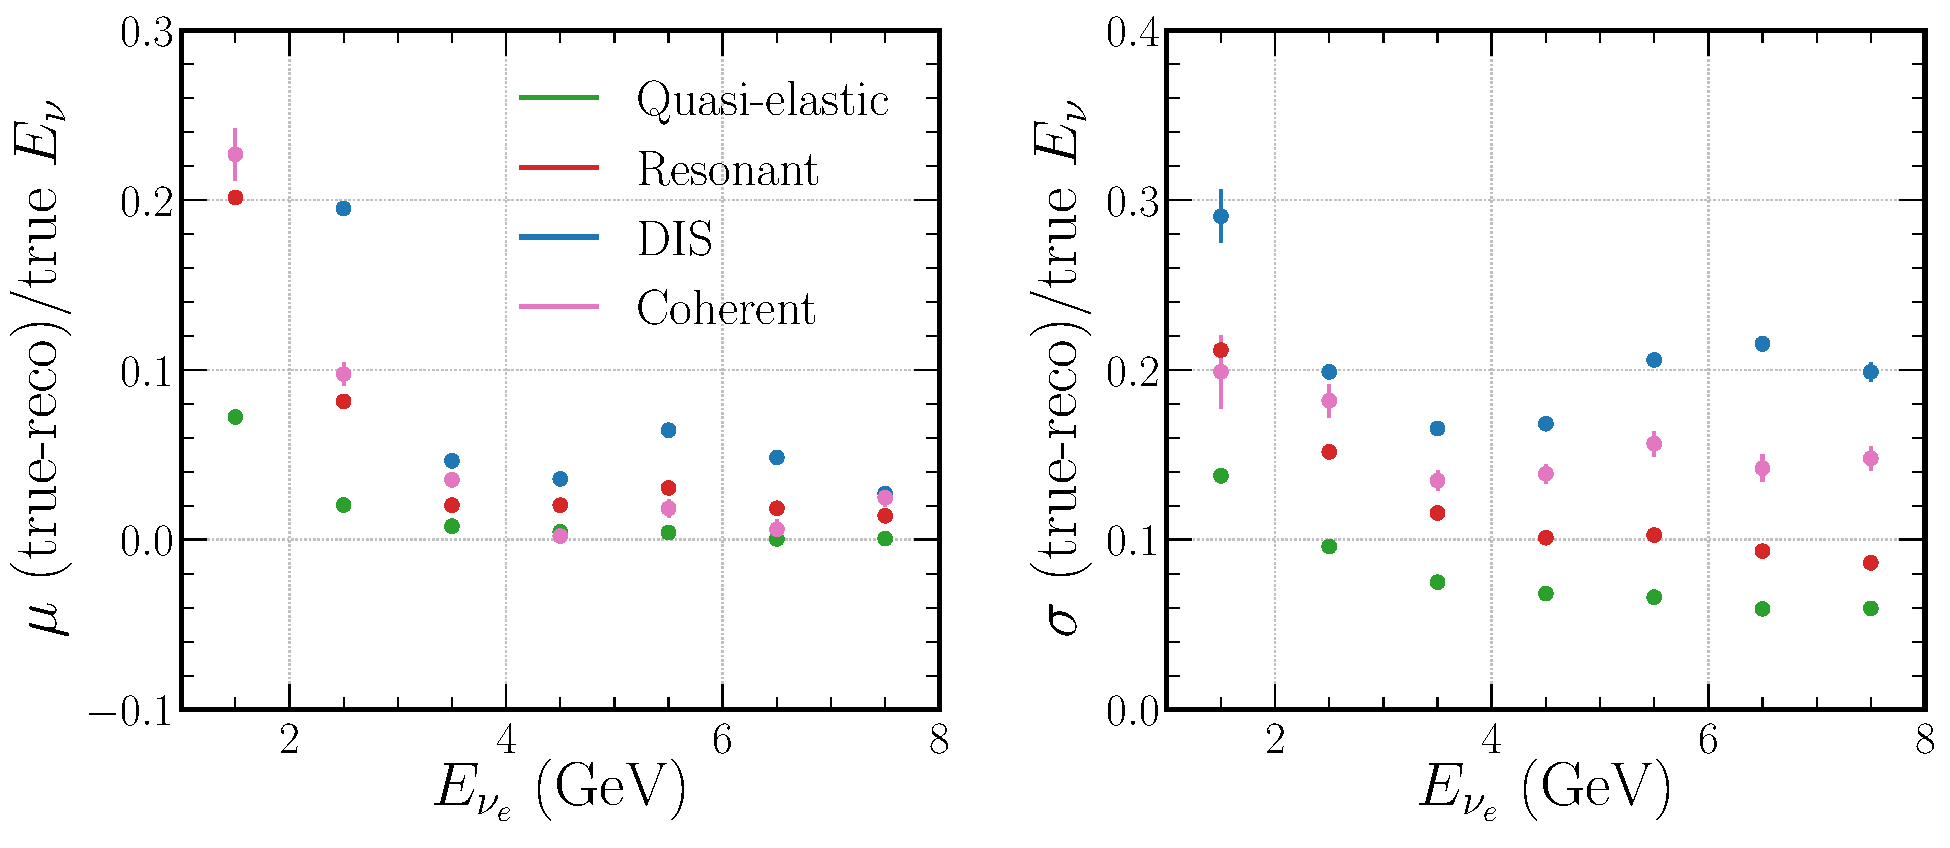
\includegraphics[width=0.8\textwidth]{diagrams/6-cvn/chipsnet/final_energy_nuel.pdf}
    \caption[final energy nuel short]
    {final energy nuel long}
    \label{fig:final_energy_nuel}
\end{figure}

\begin{figure} % FINAL NUMU ENERGY DIAGRAM %
    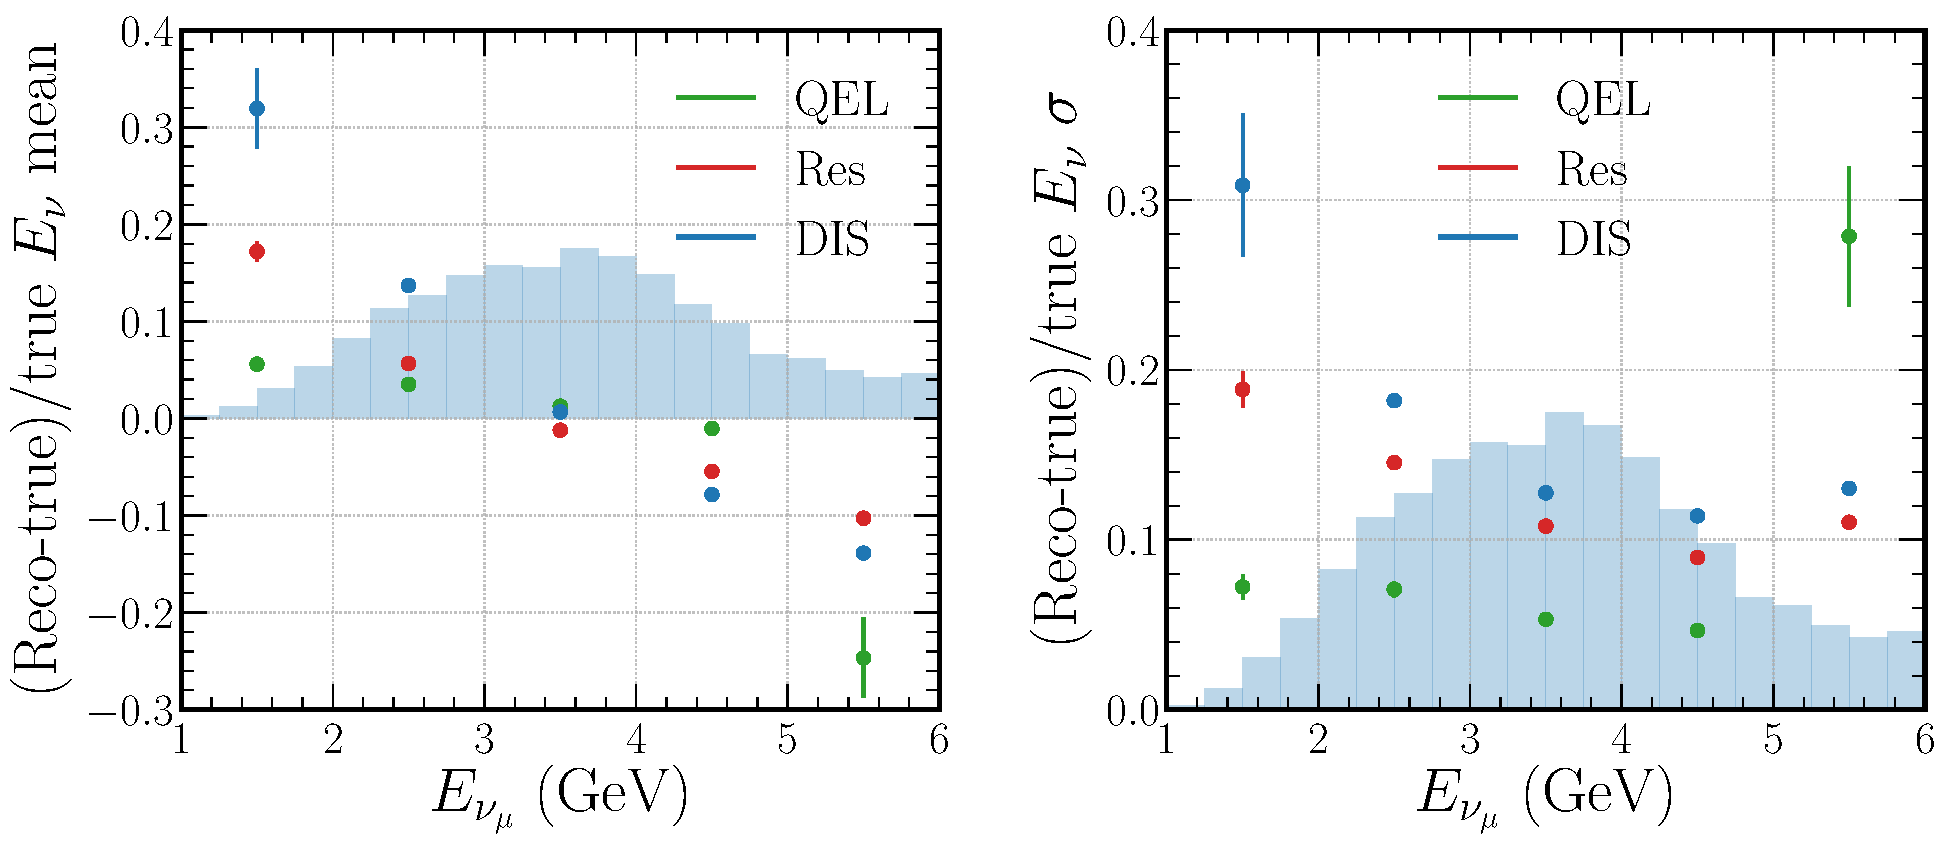
\includegraphics[width=0.8\textwidth]{diagrams/6-cvn/chipsnet/final_energy_numu.pdf}
    \caption[final energy numu short]
    {final energy numu long}
    \label{fig:final_energy_numu}
\end{figure}

\subsection{Combined performance} %%%%%%%%%%%%%%%%%%%%%%%%%%%%%%%%%%%%%%%%%%%%%%%%%%%%%%%%%%%%%%%%
\label{sec:cvn_results_combined} %%%%%%%%%%%%%%%%%%%%%%%%%%%%%%%%%%%%%%%%%%%%%%%%%%%%%%%%%%%%%%%%%

INFO: Table of the final number of expected events and efficiency and purity of the signal at the
chosen cut value (nuel and numu)
INFO: Super-k/Dune/Nova comparison numbers for efficiencies and energy resolutions etc...

\begin{figure} % FINAL NUEL ENERGY DIST DIAGRAM %
    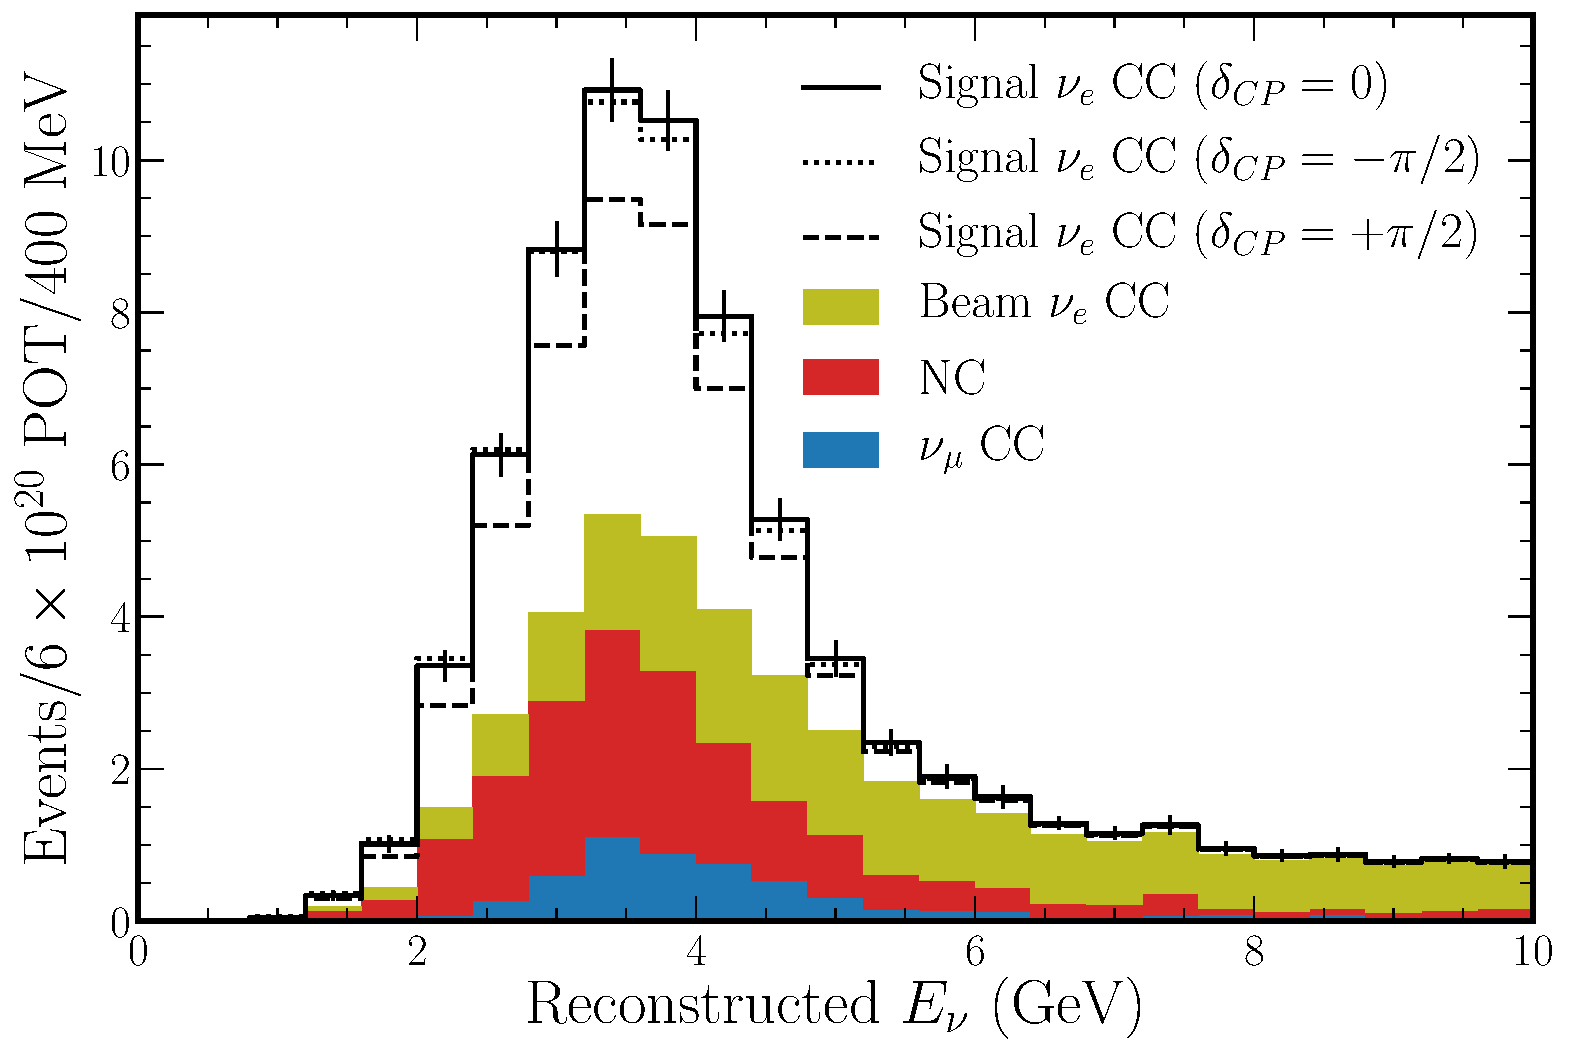
\includegraphics[width=0.7\textwidth]{diagrams/6-cvn/chipsnet/final_nuel_passed_energy_dist.pdf}
    \caption[final nuel passed energy dist short]
    {final nuel passed energy dist long}
    \label{fig:final_nuel_passed_energy_dist}
\end{figure}

\begin{figure} % FINAL NUMU ENERGY DIST DIAGRAM %
    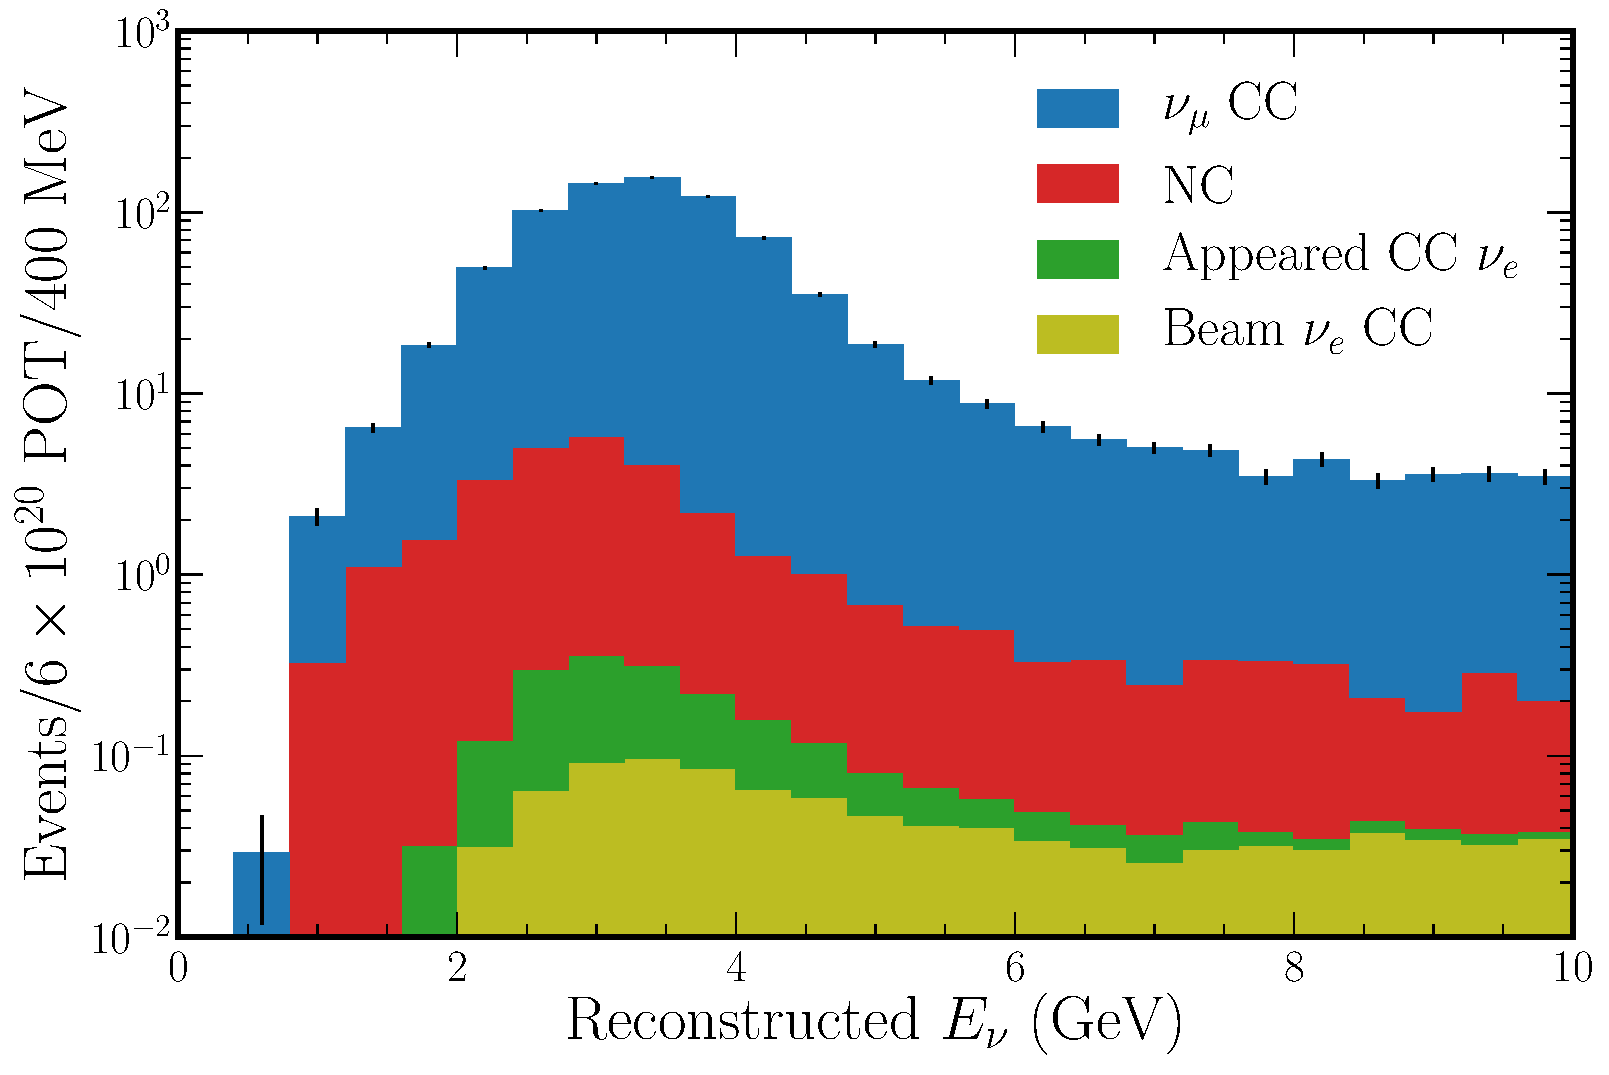
\includegraphics[width=0.7\textwidth]{diagrams/6-cvn/chipsnet/final_numu_passed_energy_dist.pdf}
    \caption[final numu passed energy dist short]
    {final numu passed energy dist long}
    \label{fig:final_numu_passed_energy_dist}
\end{figure}

\subsection{Comparison with standard methods} %%%%%%%%%%%%%%%%%%%%%%%%%%%%%%%%%%%%%%%%%%%%%%%%%%%%
\label{sec:cvn_results_comparison} %%%%%%%%%%%%%%%%%%%%%%%%%%%%%%%%%%%%%%%%%%%%%%%%%%%%%%%%%%%%%%%

- BIG UP the difference in time it takes, as this can have a huge impact on reprocessing your full
dataset
- This allows a massive increase in the iteration rate of analysis, which can lead to an improved
rate of improvement, with less time wasted.

INFO: Need to understand the error on the number of cosmic passing the cut, is it reasonable
without a huge amount of testing data?
INFO: What are the errors on all my number values? with the stats I have?
- Having a veto in the upstream towards the beam direction would be best
- Talk about how beam muons upstream of the detector are just like cosmics and say how they could
be rejected aswell
INFO: proof that there is no topological difference between QEL and MEC if we are combining them
for the energy stuff
- Position of PMTs does not seem to be that important

- Nova gets about ~7percent energy resolution for signal events
in Ref.~\cite{jiang2019}
- Fitqun gets ~20cm vertex position resolution for nuel CCQE events
- Fitqun gets ~16cm vertex position resolution for numu CCQE events
- Fitqun gets 5.39percent to 2.58percent lepton energy resolution for nuel CCQE events
- Fitqun gets ~2.5percent lepton energy resolution for numu CCQE events
- Note all the stuff in super-k happens at lower energies ~<1.4GeV

\section{Explainability} %%%%%%%%%%%%%%%%%%%%%%%%%%%%%%%%%%%%%%%%%%%%%%%%%%%%%%%%%%%%%%%%%%%%%%%%%
\label{sec:cvn_explain} %%%%%%%%%%%%%%%%%%%%%%%%%%%%%%%%%%%%%%%%%%%%%%%%%%%%%%%%%%%%%%%%%%%%%%%%%%

- Simple PCA REF was also tried, but t-SNE was found to work much better as expected.

\begin{figure} % COSMIC t-SNE DIAGRAM %
    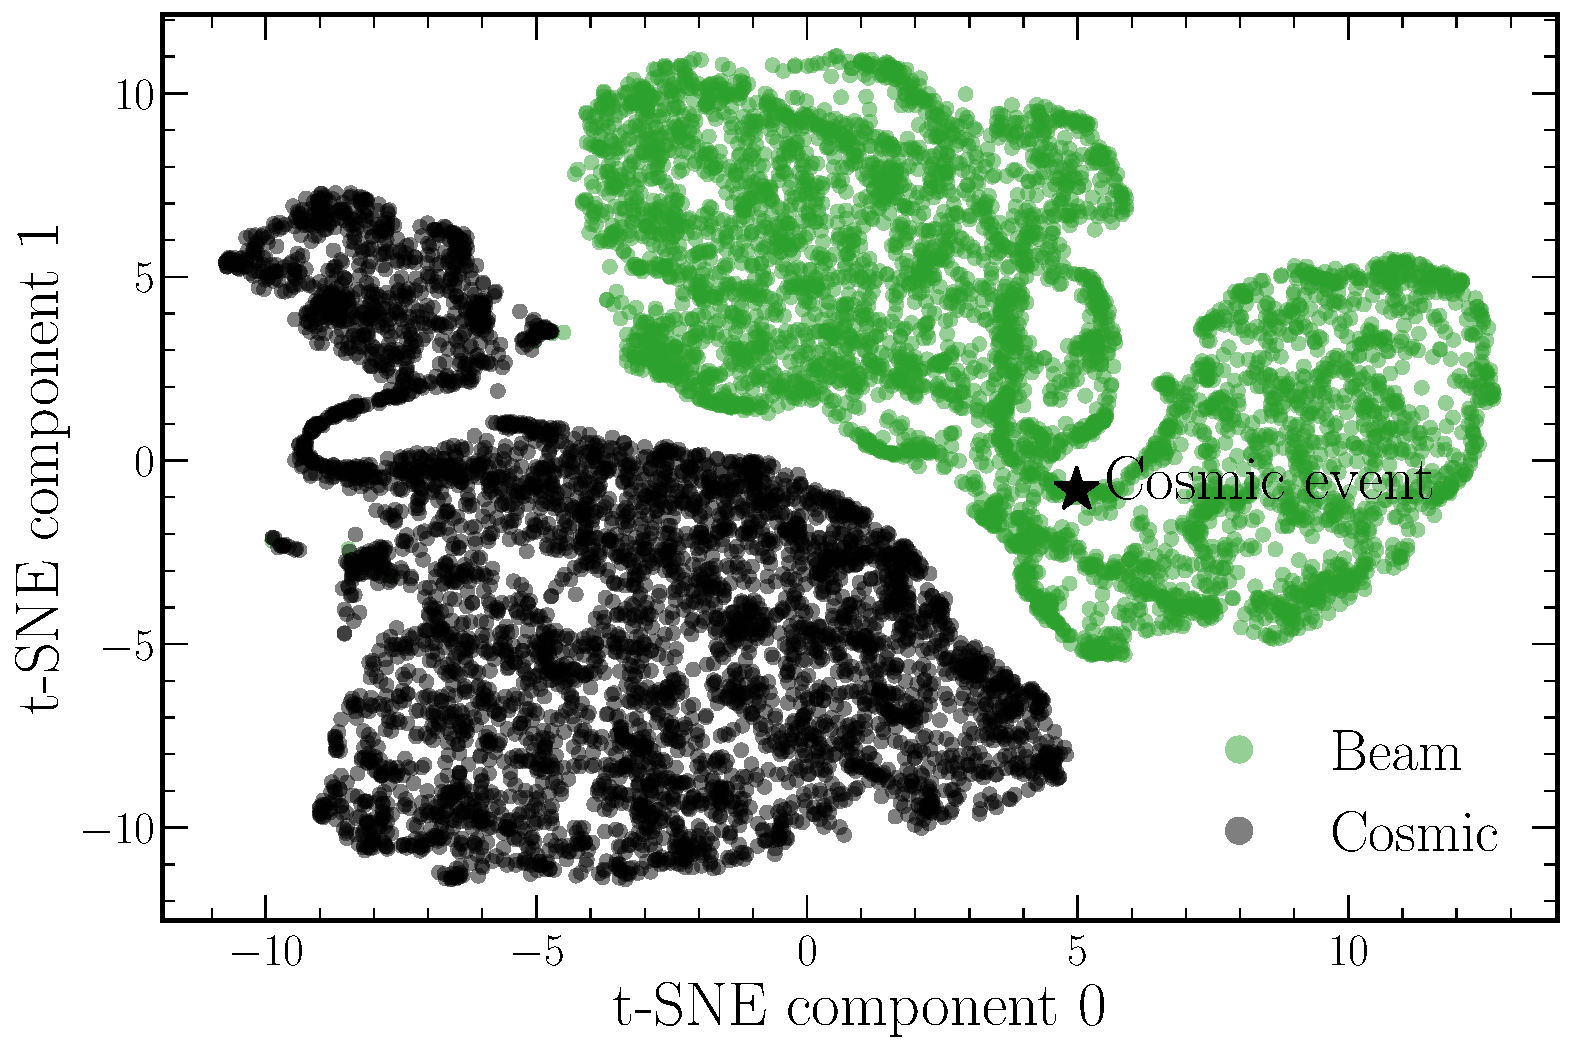
\includegraphics[width=0.7\textwidth]{diagrams/6-cvn/chipsnet/final_cosmic_tsne.pdf}
    \caption[final cosmic tsne short]
    {final cosmic tsne long}
    \label{fig:final_cosmic_tsne}
\end{figure}

\begin{figure} % BEAM t-SNE DIAGRAM %
    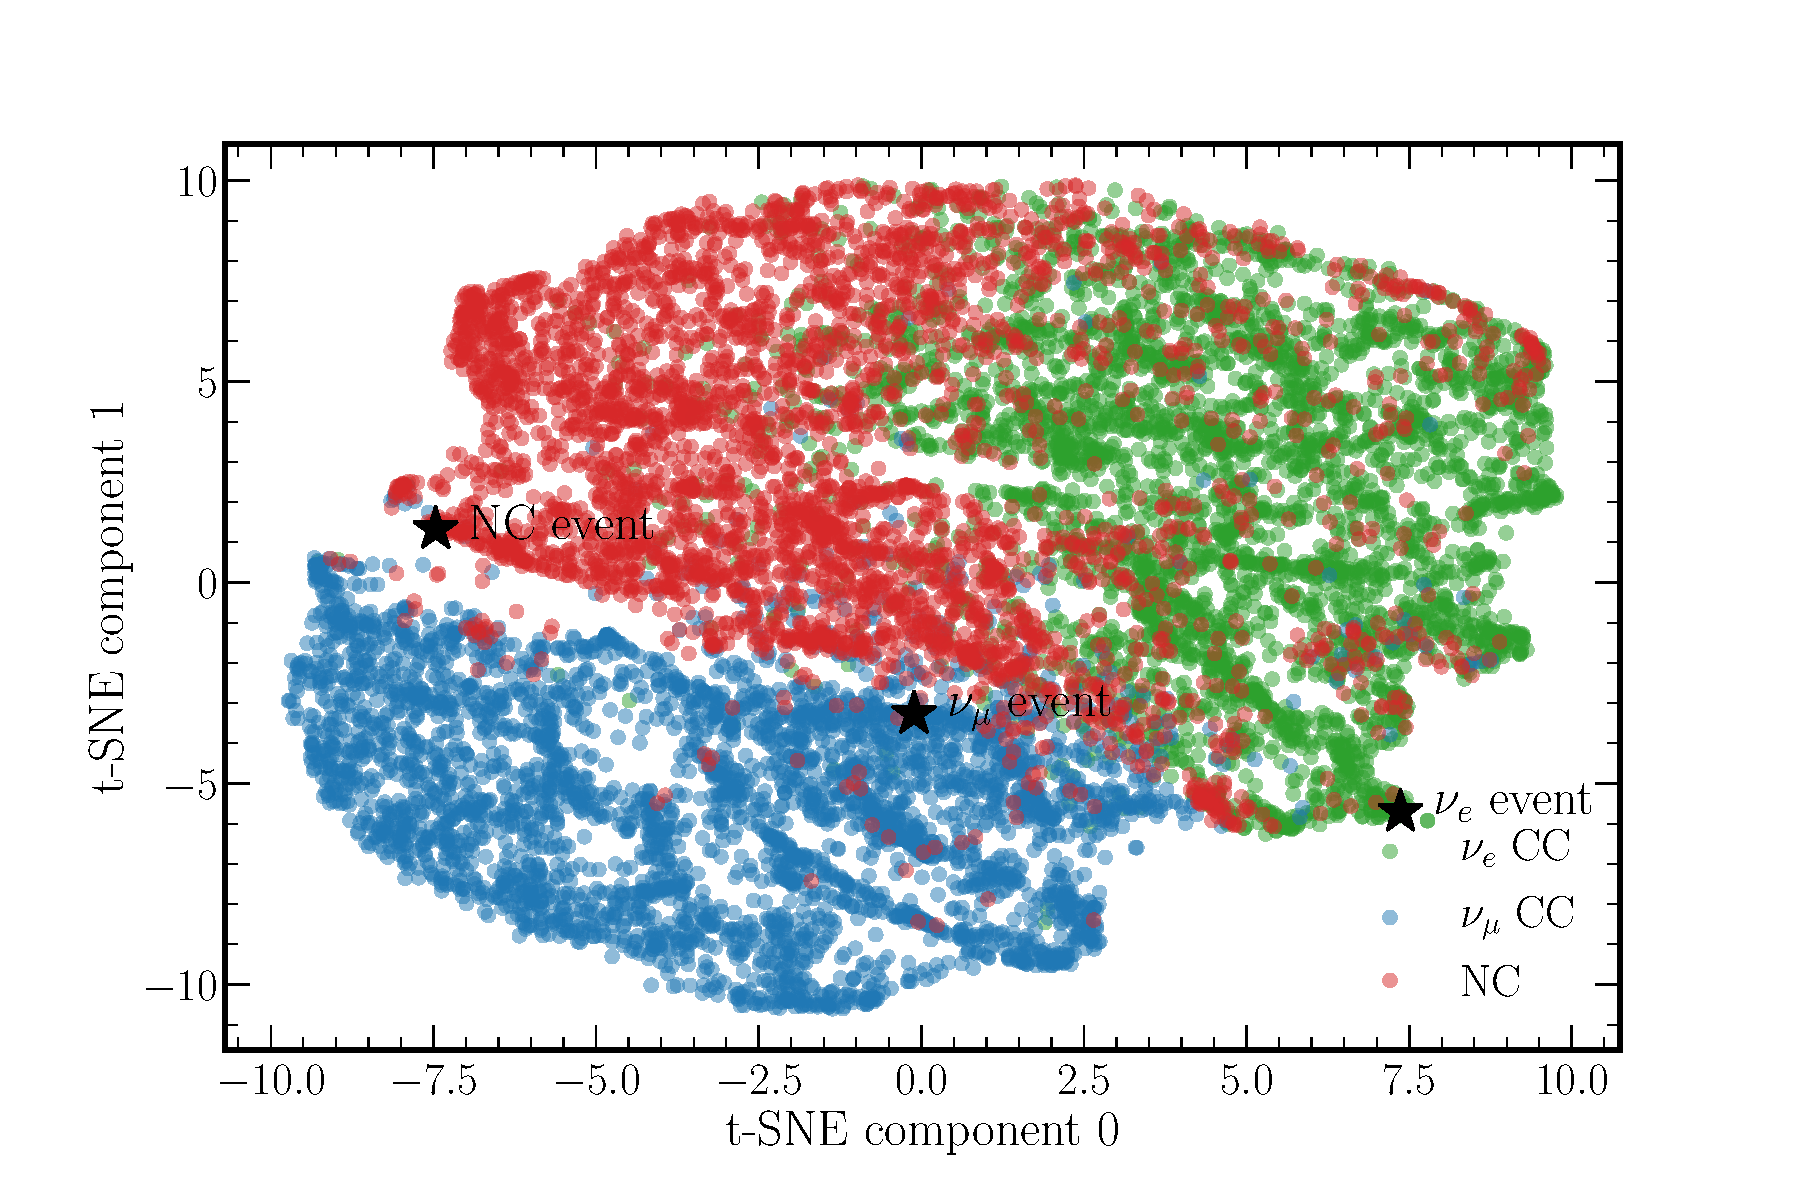
\includegraphics[width=0.7\textwidth]{diagrams/6-cvn/chipsnet/final_beam_tsne.pdf}
    \caption[final beam tsne short]
    {final beam tsne long}
    \label{fig:final_beam_tsne}
\end{figure}

\begin{figure} % BEAM t-SNE EVENTS DIAGRAM %
    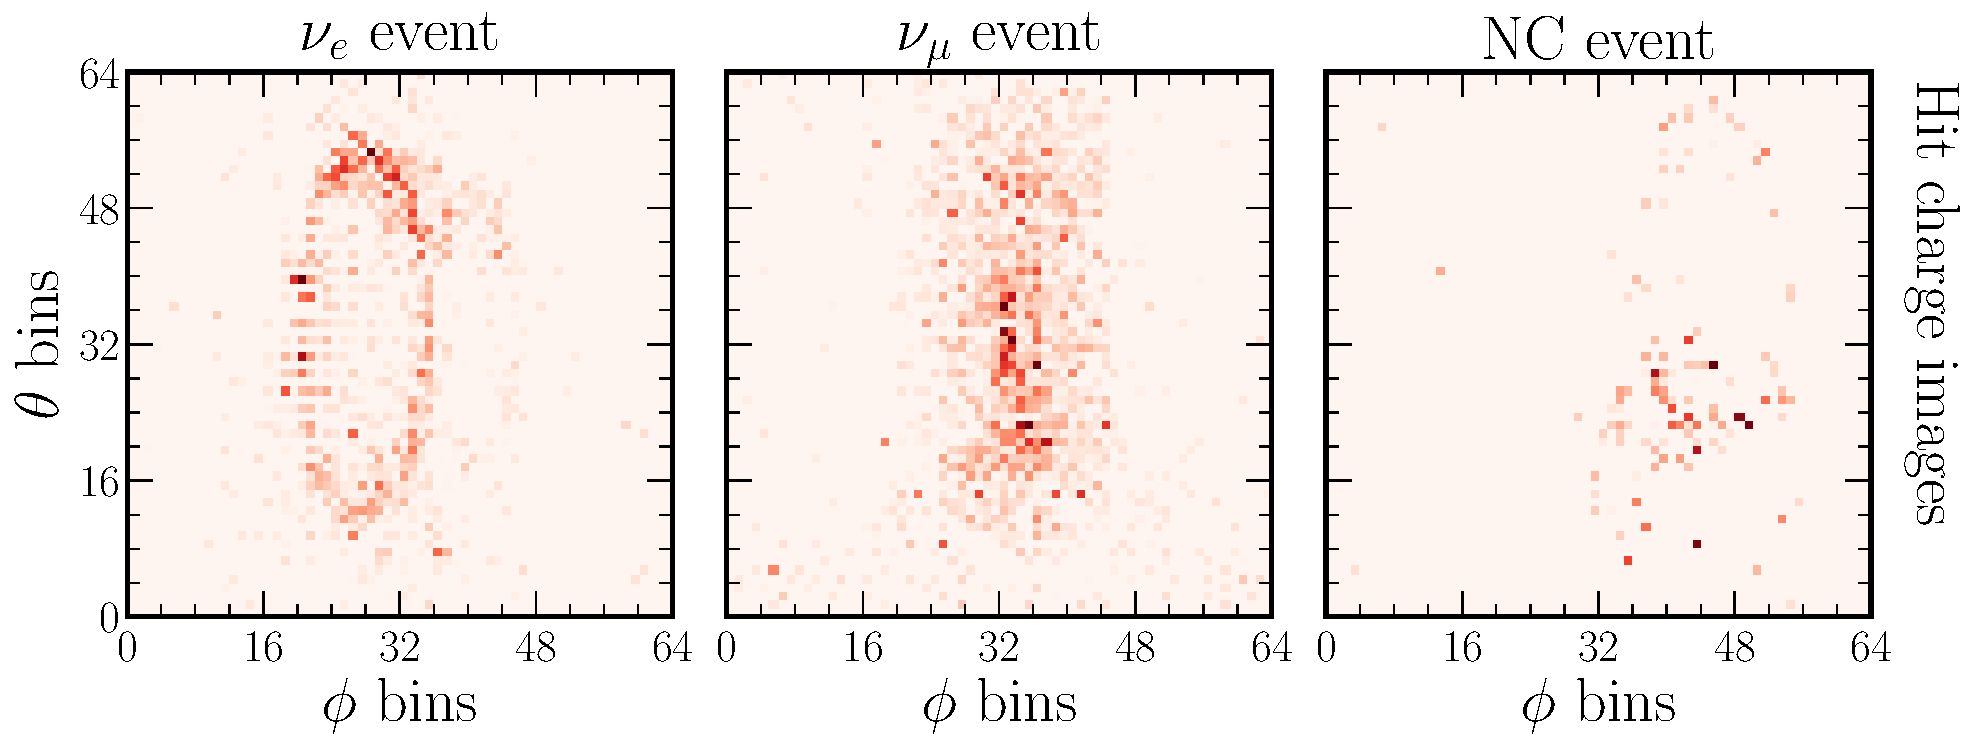
\includegraphics[width=\textwidth]{diagrams/6-cvn/chipsnet/final_beam_tsne_events.pdf}
    \caption[final beam tsne events short]
    {final beam tsne events long}
    \label{fig:final_beam_tsne_events}
\end{figure}

\begin{figure} % FRAC ENERGY EFF DIAGRAM %
    \includegraphics[width=0.7\textwidth]{diagrams/6-cvn/chipsnet/final_frac_energy_eff.pdf}
    \caption[final frac energy eff short]
    {final frac energy eff long}
    \label{fig:final_frac_energy_eff}
\end{figure}

\begin{figure} % EXPLAIN EXAMPLE EVENT DIAGRAM %
    \includegraphics[width=\textwidth]{diagrams/6-cvn/chipsnet/explain_example_event.pdf}
    \caption[explain example event short]
    {explain example event long}
    \label{fig:explain_example_event}
\end{figure}

\begin{figure} % ACTIVATIONS DIAGRAM %
    \centering
    \subcaptionbox{explain cosmic activations\label{fig:explain_cosmic_activations}}{%
        \includegraphics[height=16cm]{diagrams/6-cvn/chipsnet/explain_cosmic_activations.pdf}%
    }
    \quad
    \subcaptionbox{explain beam activations\label{fig:explain_beam_activations}}{%
        \includegraphics[height=16cm]{diagrams/6-cvn/chipsnet/explain_beam_activations.pdf}%
    }
    \quad
    \subcaptionbox{explain energy activations\label{fig:explain_energy_activations}}{%
        \includegraphics[height=16cm]{diagrams/6-cvn/chipsnet/explain_energy_activations.pdf}%
    }
    \caption[The caption]
    {The caption}
\end{figure}

Initial CNN visualisation paper in Ref.~\cite{zeiler2013}
Original t-SNE paper in Ref.~\cite{maaten2008}

- For all the t-SNE stuff
- There have been plently of attempts at visualising high-dimensional data on a 2/3 dimensional
map, including Sammon mapping, Isomap, Locally Linear Embedding, Stochastic Neighbour Embedding.
- Older implementations tended to cluster all data points towards the centre of the map and proved
difficult to optimise.
- You basically set a summed probability between all points in the low-dimensional space to a
summed probability between all points in the high-dimensional space.
- t-SNE uses the student-t distribution (with a heavy tail) in the low-dimensional space to
calculate the probability. This alleviates both the crowding problem and is easier to optimise.
- Optimisation uses a simple momentum term, plus two new ideas. "Early compression" which forces
map points to stay close to each other at the start of optimisation, it is then easier for
clusters to move through each other and explore all possible global organisations of the data,
this is implemented as an L2-penalty term proportional to the sum of squared distances from the
origin, this is then removed at an iteration given as input. Secondly, "Early exaggeration" which
creates tight widely seperated clusters.

\section{Alternative implementations} %%%%%%%%%%%%%%%%%%%%%%%%%%%%%%%%%%%%%%%%%%%%%%%%%%%%%%%%%%%%
\label{sec:cvn_alt} %%%%%%%%%%%%%%%%%%%%%%%%%%%%%%%%%%%%%%%%%%%%%%%%%%%%%%%%%%%%%%%%%%%%%%%%%%%%%%

The work outlined in this chapter is the result of extensive testing and optimisation of many
differing approaches to applying CNNs to \chips. Here we highlight some interesting findings from
this process to both provide completeness, but also to hopefully inform future work on this topic.

\subsubsection*{Alternative inputs} %%%%%%%%%%%%%%%%%%%%%%%%%%%%%%%%%%%%%%%%%%%%%%%%%%%%%%%%%%%%%%

There are many possible event representations that can be used as input to the CNNs in this work.
Three different approaches are explored in this work!

- New ideas with x+ x- mapping in Ref.~\cite{berns2020}
- Fraction of deposited charge in endcaps = 0.4769380479133997

\begin{equation} % ISO CASE EQUATION %
    X_{\pm}=
    \begin{cases}
        1-\chi_{\mp} & (z \geq 0) \\
        \chi_{\pm}   & (z < 0)
    \end{cases}
    \label{eq:iso_case}
\end{equation}

\begin{equation} % ISO MAIN EQUATION %
    \chi_{\pm}=W(\rho,z)\frac{\pi\pm\phi}{2\pi}
    \label{eq:iso_main}
\end{equation}

\begin{equation} % ISO PART EQUATION %
    W(\rho,z)=\sqrt{\frac{\rho^{2}-2R|z|+RH}{R^{2}+RH}}
    \label{eq:iso_part}
\end{equation}

- where R and Z are the radius and height of the detector cylinder and W is chosen for constant
surface density.
- Turns out removing the distortions of not viewing the event from the vertex is the most
important thing!!!

- Approaches in the past for event classification using CNNs for water cherenkov detectors have
taken a few Approaches to generating the input image representation.
- Projecting onto a 2d surface "outside" the detector

\begin{table}
    \begin{tabular}{cccc}
        Metric                   & Vertex View & Origin Raw View & Origin Iso View \\
        \midrule
        Maximum FOM              & 0.461       & 0.422           & 0.419           \\
        Highest Score Efficiency & 0.878       & 0.874           & 0.867           \\
        Highest Score Purity     & 0.354       & 0.291           & 0.298           \\
        ROC Integral             & 0.825       & 0.822           & 0.821           \\
        PRC Integral             & 0.707       & 0.675           & 0.670           \\
    \end{tabular}
    \caption[Comparison of performance metrics for three input image representations.]
    {Comparison of performance metrics for the three input image representations considered. The
        highest score selection uses the highest scoring output neuron for classification. The ROC
        and PRC integrals are taken from the curves shown in
        Fig.~\ref{fig:repr_nuel_comp_curves}.}
    \label{tab:repr}
\end{table}

\begin{figure} % REPR NUEL EFF CURVES DIAGRAM %
    \includegraphics[width=0.7\textwidth]{diagrams/6-cvn/chipsnet/repr_nuel_eff_curves.pdf}
    \caption[CC $\nu_{e}$ efficiency and purity curves for the three input image representations.]
    {CC $\nu_{e}$ efficiency, purity and $\mathrm{efficiency}\times\mathrm{purity}$ for different
        values of CC $\nu_{e}$ score selection for the three input image representations
        considered. The \emph{vertex view} curves are shown by the solid lines, the \emph{origin
            raw view} curves by the dashed lines, and the \emph{origin dotted} surves by the dotted
        lines.}
    \label{fig:repr_nuel_eff_curves}
\end{figure}

\begin{figure} % REPR NUEL COMP CURVES DIAGRAM %
    \includegraphics[width=0.8\textwidth]{diagrams/6-cvn/chipsnet/repr_nuel_comp_curves.pdf}
    \caption[Comparison curves for the three input image representations considered.]
    {Comparison curves for the three input image representations considered. Signal vs background
        selection efficiencies as the CC $\nu_{e}$ score selection is varied (left). Signal CC
        $\nu_{e}$ purity vs efficiency as the CC $\nu_{e}$ score selection is varied (right). The
        \emph{vertex view} curves are shown by the solid lines, the \emph{origin raw view} curves
        by the dashed lines, and the \emph{origin dotted} curves by the dotted lines. The left
        plot contains what are commonly referred to as receiver-operator curves (ROC), while the
        right plot contains precision-recall (PRC) curves.}
    \label{fig:repr_nuel_comp_curves}
\end{figure}

\begin{table}
    \begin{tabular}{cccc}
        Metric                   & Charge & Charge+Time & Charge+Time+Hough \\
        \midrule
        Maximum FOM              & 0.436  & 0.461       & 0.465             \\
        Highest Score Efficiency & 0.869  & 0.878       & 0.877             \\
        Highest Score Purity     & 0.357  & 0.354       & 0.369             \\
        ROC Integral             & 0.824  & 0.825       & 0.826             \\
        PRC Integral             & 0.689  & 0.707       & 0.712             \\
    \end{tabular}
    \caption[Comparison of performance metrics for each additional input image map.]
    {Comparison of performance metrics for each additional input image map. The highest score
        selection uses the highest scoring output neuron for classification.}
    \label{tab:chan}
\end{table}

\subsubsection*{Alternative training samples} %%%%%%%%%%%%%%%%%%%%%%%%%%%%%%%%%%%%%%%%%%%%%%%%%%%%

\begin{figure} % REPR NUEL EFF CURVES DIAGRAM %
    \includegraphics[width=0.7\textwidth]{diagrams/6-cvn/chipsnet/sample_nuel_eff_curves.pdf}
    \caption[CC $\nu_{e}$ efficiency and purity curves for the different training samples.]
    {CC $\nu_{e}$ efficiency, purity and $\mathrm{efficiency}\times\mathrm{purity}$ for different
        values of CC $\nu_{e}$ score selection for the different training samples considered. The
        \emph{vertex view} curves are shown by the solid lines, the \emph{origin raw view} curves
        by the dashed lines, and the \emph{origin dotted} surves by the dotted lines.}
    \label{fig:sample_nuel_eff_curves}
\end{figure}

\begin{figure} % REPR NUEL COMP CURVES DIAGRAM %
    \includegraphics[width=0.8\textwidth]{diagrams/6-cvn/chipsnet/sample_nuel_comp_curves.pdf}
    \caption[Comparison curves for the different training samples considered.]
    {Comparison curves for the different training samples considered. Signal vs background
        selection efficiencies as the CC $\nu_{e}$ score selection is varied (left). Signal CC
        $\nu_{e}$ purity vs efficiency as the CC $\nu_{e}$ score selection is varied (right). The
        \emph{flux+uniform} curves are shown by the solid lines, the \emph{flux} curves by the
        dashed lines, and the \emph{uniform} curves by the dotted lines. The left plot contains
        what are commonly referred to as receiver-operator curves (ROC), while the right plot
        contains precision-recall (PRC) curves.}
    \label{fig:sample_nuel_comp_curves}
\end{figure}

\begin{table}
    \begin{tabular}{cccc}
        Metric                   & Flux  & Uniform & Flux+Uniform \\
        \midrule
        Maximum FOM              & 0.465 & 0.339   & 0.386        \\
        Highest Score Efficiency & 0.877 & 0.799   & 0.834        \\
        Highest Score Purity     & 0.369 & 0.347   & 0.368        \\
        ROC Integral             & 0.826 & 0.815   & 0.820        \\
        PRC Integral             & 0.712 & 0.568   & 0.634        \\
    \end{tabular}
    \caption[Comparison of performance metrics for the different training samples considered.]
    {Comparison of performance metrics for the different training samples considered. The highest
        score selection uses the highest scoring output neuron for classification.}
    \label{tab:sample}
\end{table}

\subsubsection*{Alternative architectures} %%%%%%%%%%%%%%%%%%%%%%%%%%%%%%%%%%%%%%%%%%%%%%%%%%%%%%%

- truncated versions of the other networks so they have approximately the same number of
parameters to train for making a good comparison.

\begin{table}
    \begin{tabular}{ccccc}
        Metric                   & VGG        & Inception  & ResNet     & Inception-ResNet \\
        \midrule
        Number of parameters     & 17,225,296 & 16,893,216 & 16,526,288 & 17,145,238       \\
        Iteration time (ms)      & 88         & 192        & 112        & 209              \\
        Maximum FOM              & 0.465      & 0.459      & 0.445      & 0.444            \\
        Highest Score Efficiency & 0.877      & 0.870      & 0.869      & 0.874            \\
        Highest Score Purity     & 0.369      & 0.373      & 0.374      & 0.349            \\
        ROC Integral             & 0.825      & 0.825      & 0.824      & 0.824            \\
        PRC Integral             & 0.712      & 0.706      & 0.688      & 0.699            \\
    \end{tabular}
    \caption[Comparison of performance metrics for the different network architectures considered.]
    {Comparison of performance metrics the different network architectures considered. The highest
        score selection uses the highest scoring output neuron for classification.}
    \label{tab:arch}
\end{table}

\subsubsection*{Alternative beam categorisation} %%%%%%%%%%%%%%%%%%%%%%%%%%%%%%%%%%%%%%%%%%%%%%%%%

- The choice of categorisation can matter
- All categories CC QE, Res, DIS, Coh, MEC, and other for both $\nu_{e}$ and $\nu_{\mu}$, plus NC
Res, DIS, Coh, and other, for a total of 16 categories. You can then sum the scores as Nova have
done etc.... to get the combined categories
- Fully combined, you may think would work better as it just focuses on what we want to optimise.
This is CC $\nu_{e}$, CC $\nu_{\mu}$, and NC.
- Combined plus the CC and NC cats that are masked like in this work described above.

\begin{table}
    \begin{tabular}{cccc}
        Metric                   & All   & Full-Comb & Multi (learnt) \\
        \midrule
        Maximum FOM              & 0.465 & 0.451     & 0.471          \\
        Highest Score Efficiency & 0.877 & 0.871     & 0.872          \\
        Highest Score Purity     & 0.369 & 0.359     & 0.392          \\
        ROC Integral             & 0.826 & 0.825     & 0.826          \\
        PRC Integral             & 0.712 & 0.692     & 0.716          \\
    \end{tabular}
    \caption[Comparison of performance metrics for the different beam categorisations considered.]
    {Comparison of performance metrics for the different beam categorisations considered. The highest
        score selection uses the highest scoring output neuron for classification.}
    \label{tab:cat}
\end{table}
